\documentclass{uafthesis}

\usepackage{fixltx2e} % At the least, allows \(\) in captions.
\usepackage{ppl} % Bitches love the Paladino font.
\usepackage{amsmath, amssymb, amsfonts} % Thanks, AMS!
\usepackage{graphicx, float, subfig} % Graphics stuff
%\usepackage{epstopdf} % Should let me include eps images. Requires write18?
\usepackage{verbatim} % Mostly for the comment environment.
%\usepackage{chapterbib} % This is an option for those bundling papers.
\usepackage{minted} % Syntax hilighting!
\usepackage{ulem} % This is mostly for sout.
\usepackage[square]{natbib}
%\usepackage{tocbibind} % This fixes the "bibliography in ToC" problem that those
                       % asshole physicists said should be fixed by directly
                       % hacking the .toc file. Use with chapterbib.

%Custom macros go here.

\newcommand{\Ei}{\textrm{Ei}} % Exponential integral
\newcommand{\Eig}{\textrm{Eig}} % Eigenvalues
\newcommand{\e}[0]{\hat{e}} % Unit vector
\newcommand{\norm}[1]{\left|\left|{#1}\right|\right|} % |n|
\newcommand{\fracflat}[2]{\left.{#1}\middle/{#2}\right.} % flat fractions
\newcommand{\flatfrac}[2]{\left.{#1}\middle/{#2}\right.} % flat fractions


\begin{document}

\title{The Measurement of Anisotropic Thermal Conductivity in Snow With Needle Probes}
\author{Joshua Holbrook}

\degreeyear{2011}
\degreemonth{May}
\degree{Master of Science}
\department{Dept. of Mechanical Engineering}
\numberofmembers{3} % Make sure this is right! The grad school hates empty
                    % signature lines.
\prevdegrees{B.S.}
\college{College of Engineering and Mines}

\makesig
\maketitle

% Wondering when to use `input' and when to use `include?'
% read http://en.wikibooks.org/wiki/LaTeX/Basics#Big_Projects .
\begin{abstract}
  \input abstract.tex
\end{abstract}


%Table of Contents and such
\tableofcontents
\listoffigures
\listoftables
\listofappendices
%\listofothermaterials

\begin{acknowledgements}
  \input acknowledgements.tex
\end{acknowledgements}

\begin{quotepage}
  \input quotepage.tex
\end{quotepage}

\chapter{Introduction}
\label{sec:introduction}
\bigskip

\section{Motivation}
\label{sec:introduction:motivation}

\marginpar{Expand on this? Cite research tackling this problem through other means?}

The thermal properties of snow are of interest to scientists studying Arctic and
sub-Arctic climates because, during the long, cold winters in this region,
snow's thermal behavior plays a critical role in determining the net energy
balance between Earth's surface and the atmosphere. After all, any heat transfer
occurring between the Earth and the atmosphere over snow-covered ground must go
through the snow first (Figure \ref{fig:climate}). In fact, the snow
itself may store and release energy over time.

\begin{figure}[h]
\centering
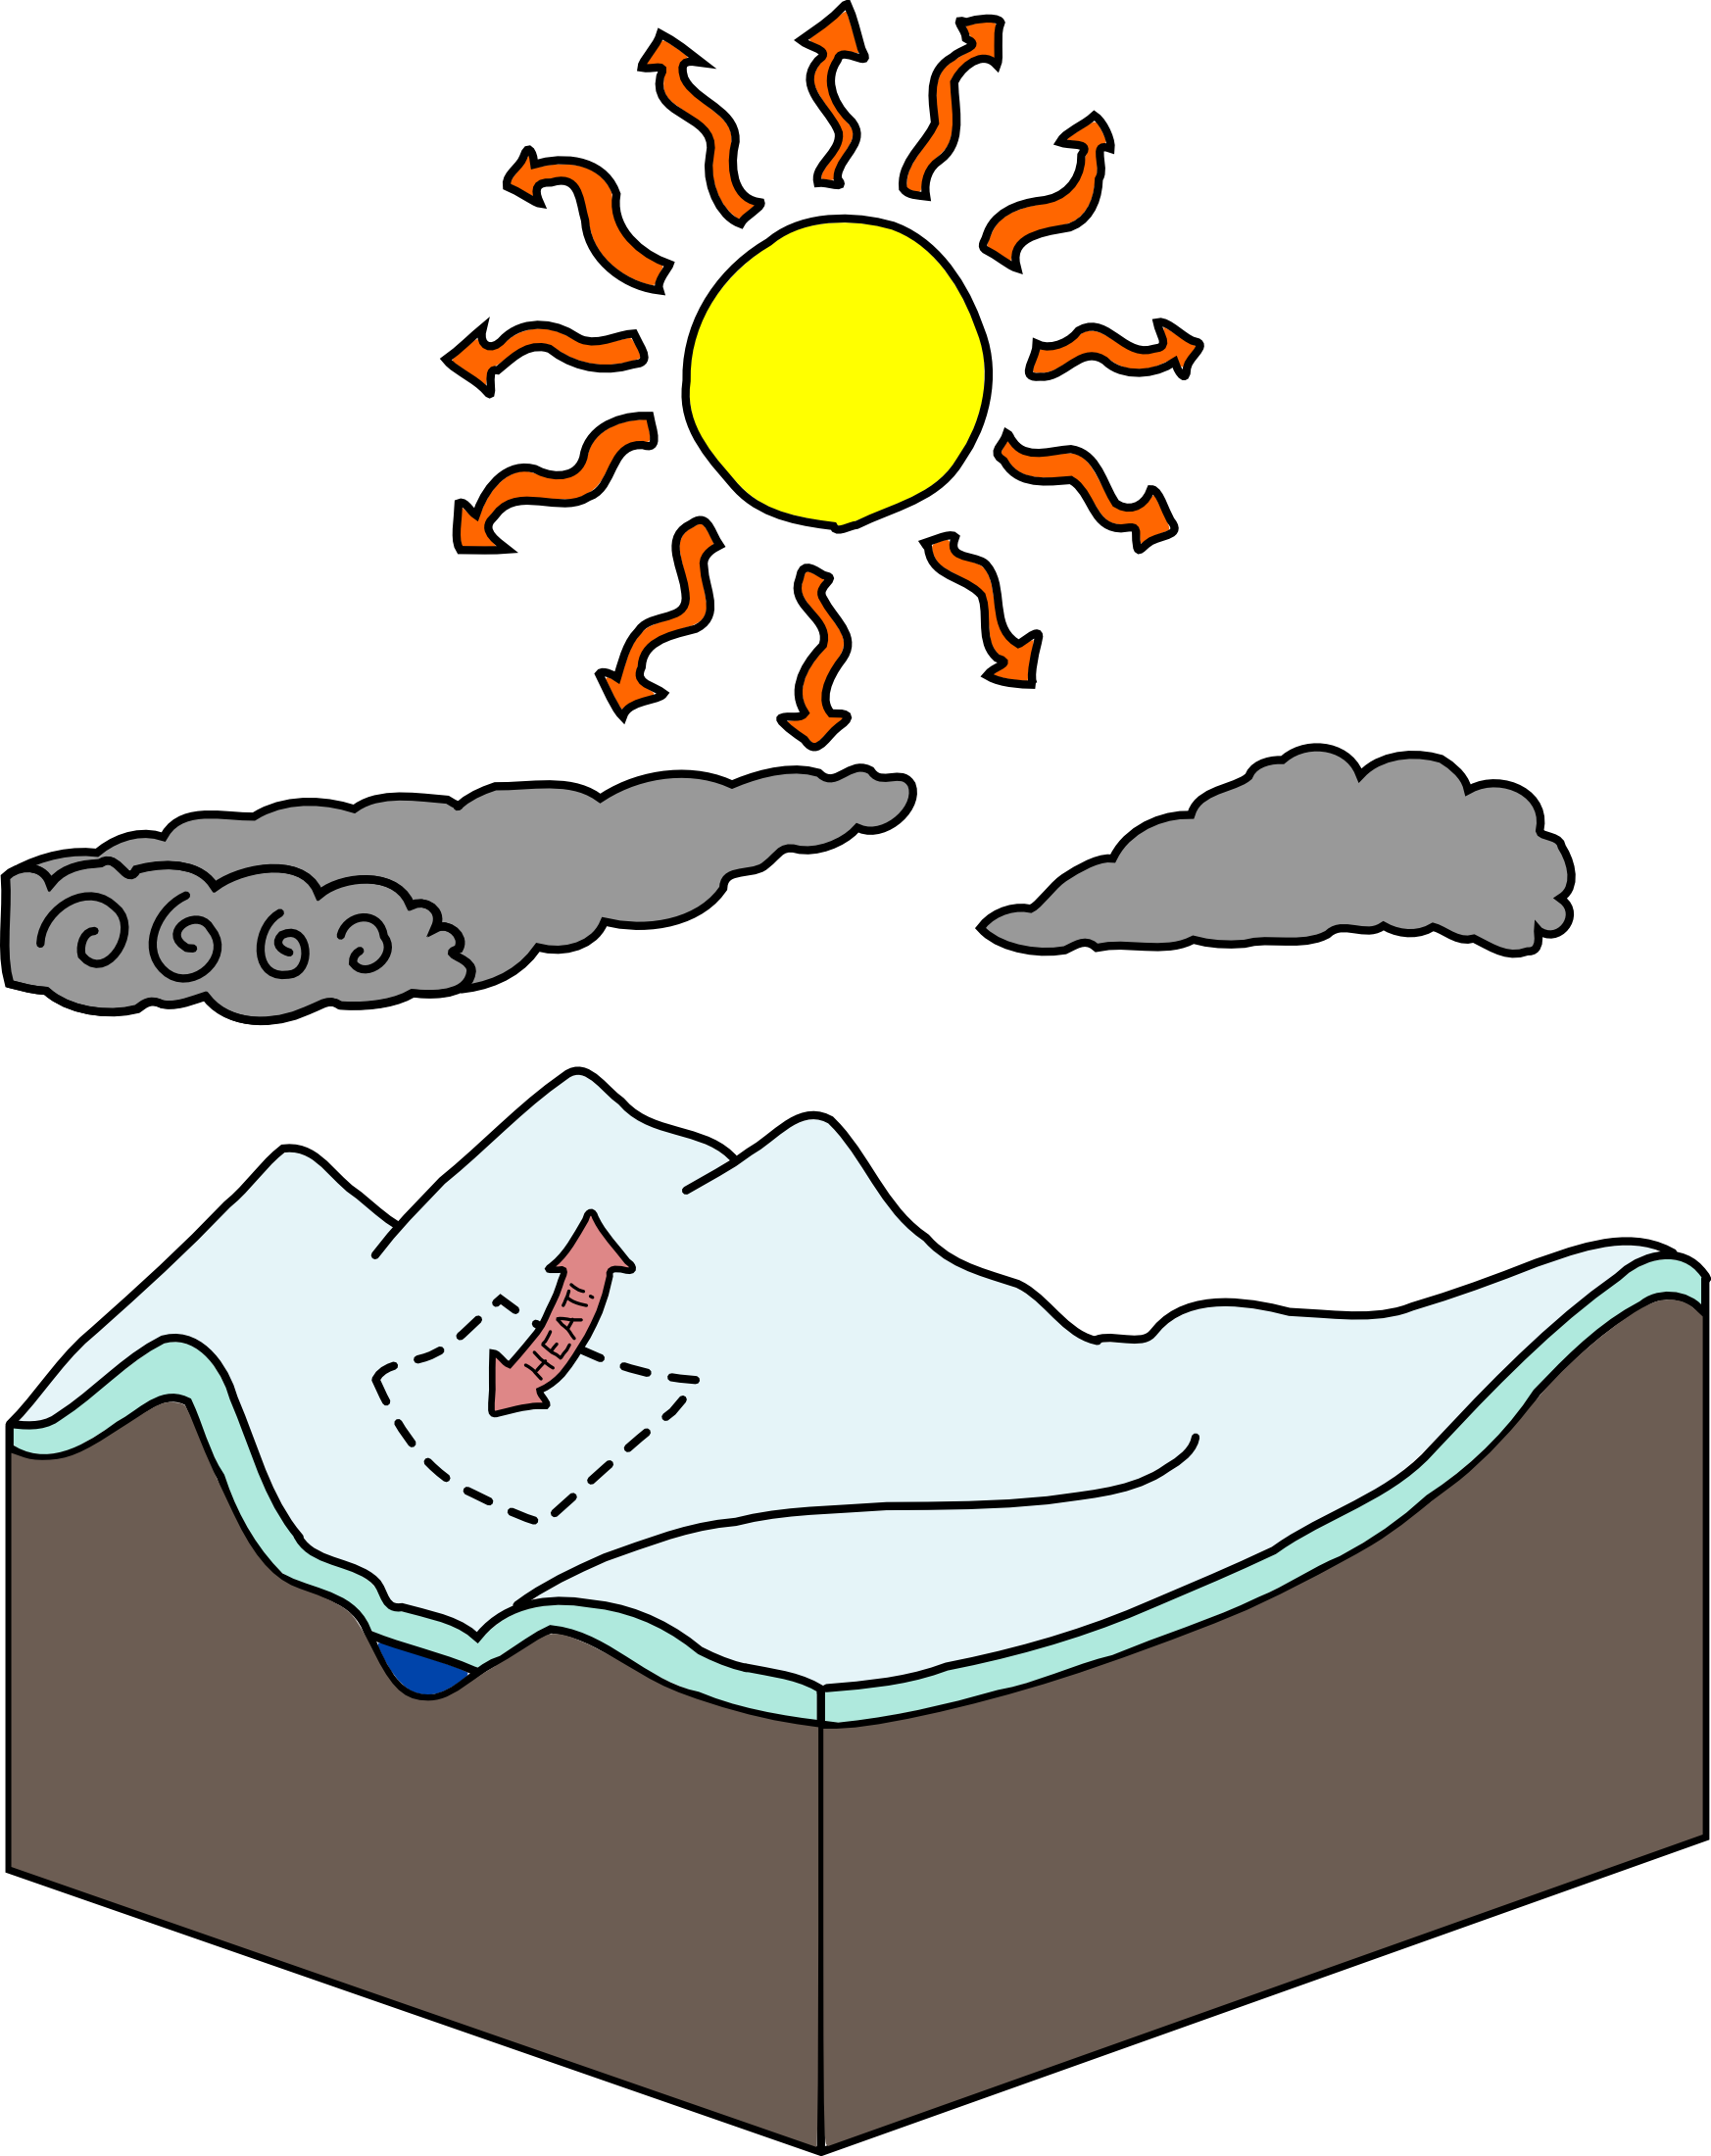
\includegraphics[width=0.4\textwidth]{fig/climate.png}
\label{fig:climate}
\caption{Arctic and Sub-Arctic climate is affected largely by heat transfer
between the atmosphere and the ground. Snowpack adds thermal resistance
transfer, affecting this heat transfer.}
\end{figure}

This energy transfer is critical in accurate climate models for these cold
regions, therefore the effective thermal conductivity of snow is a very
important factor for these models, and has been studied thoroughly \cite{sturm1, sturm2, sturm3}.


\section{Needle Probes: Basic Principles}
\label{sec:introduction:needles}

A more typical technique for measuring thermal conductivity, especially in the
context of engineering materials such as building insulation, is the guarded
hot plate. For this technique, a constant temperature gradient is induced across
the material, and heat flux over the material is measured.  By Fourier's Law,
\(k = \frac{\dot{q}l}{A\Delta T}\), where \(\dot{q}\) is the heat flux, \(A\) is
the cross-sectional area of the sample, \(l\) is the sample thickness, and 
\(\Delta T\) is the temperature difference across the sample. This technique
works great in many cases. However, it is difficult to take guarded hot plate
measurements of snow because it changes structure immediately after virtually
any physical interaction.

Another technique used for porous materials, such as soils and snow, is the
needle probe method. A needle probe consists of a long, thin needle with heating
wire running along its interior, and a temperature sensor in the center. This
configuration approximates an infinite line of constant-flux heat source
(Figure \ref{fig:needle_xsect}) \cite{basictheory}.

\begin{figure}[h]
\centering
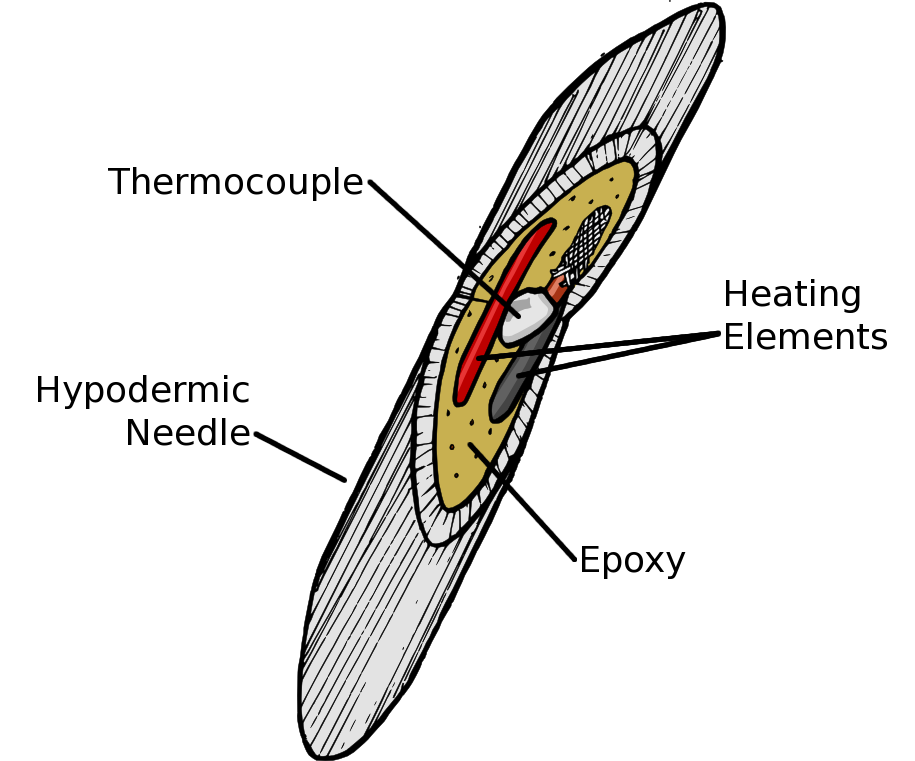
\includegraphics[width=0.2\textwidth]{fig/needle_xsect.png}
\label{fig:needle_xsect}
\caption{An illustration of a needle probe in cross-section. Note that the heat
trace in many needle probes, including the one used in experiments for this
research, actually wraps around an inner core instead of running axially through
the needle.}
\end{figure}

This needle is inserted into the material whose thermal conductivity is being
measured, and a constant voltage is applied to the needle's heating element.
This causes a constant heat flux along the needle, and, knowing the resistance
of the heat trace, this heat flux may be calculated. This causes the material's
temperature near the needle to rise (Figure \ref{fig:heating_curve}. After some
given amount of time, the heating element is turned off, and the temperature
around the needle begins to fall back towards ambient (Figure \ref{fig:cooling_curve}).
The temperature data measured over time for these two periods are called the
heating cooling curves, respectively.  Based on the slopes of these
curves as a function of \(\ln(t)\) and approximate analytical solutions for
these situations, effective thermal conductivity may be calculated.

In this document, studies concentrate on the heating curve. In fact, the
numerical and analytical approaches focus exclusively on the heating curve. This
is because the initial conditions of the cooling curve problem depend on the
final conditions of the heating curve problem, and because many references spend
more time describing the derivation of the heating curve and list the cooling
curve as being possible to derive ``from an analogous argument.'' However, the
benchtop and in-situ measurements use both heating and cooling curves.

\section{Difficulties with the Needle Probe Method}

It should be noted that the needle probe method is not without its caveats. For
instance, it was shown that convection can and will occur in natural snowpack
\cite{sturm3}. In addition to the fact that convection in snowpack can change the
entire assumed heat transfer dynamic, heating the needle itself can cause this
convection to occur. This means that, when measurements are taken, there will
not only be ``transient'' regions due to early-time behavior, but also regions
where convection becomes a major force. Practically, this means that linear
portions (with respect to \(\ln(t)\)) must be found in between these regions
of instability.

\section{Snow Metamorphic Principles}
\label{sec:introduction:metamorphic}

The structure of a snowpack is strongly influenced by outside environmental
factors. Immediately after falling from the sky, snow begins to metamporphose as
it compacts under its own weight. In addition to this, temperature gradients
cause snow to sublimate and re-form in different regions of the snowpack, in a
process called vapor transport. Vapor transport is best known for causing
depth hoar, but occurs throughout the snowpack. Other events, such as
freeze-thaw events, may also change the form of snow. All these metamorphic
processes on snow cause it to form regions of varying thermal conductivity. In
some cases, these regions may form sharp, distinct layers with constant
properties, while in other cases they have continuously varying properties.

\section{Anisotropic Aggregate Behavior in Snow}

At a macroscale, alternating regions of low-conductivity and high-conductivity
material may act in the aggregate as a single material of anisotropic thermal
conductivity---In other words, the effective thermal conductivity parallel to
the orientation of the layers may be different than the effective thermal
conductivity orthogonal to the layers.

For example, suppose a composite exists of alternating layers, each of thickness
\(l\) and with conductivities \(k_1\) and \(k_2\), as in Figure
\ref{fig:ex_laminate}:

\begin{figure}[h]
\centering
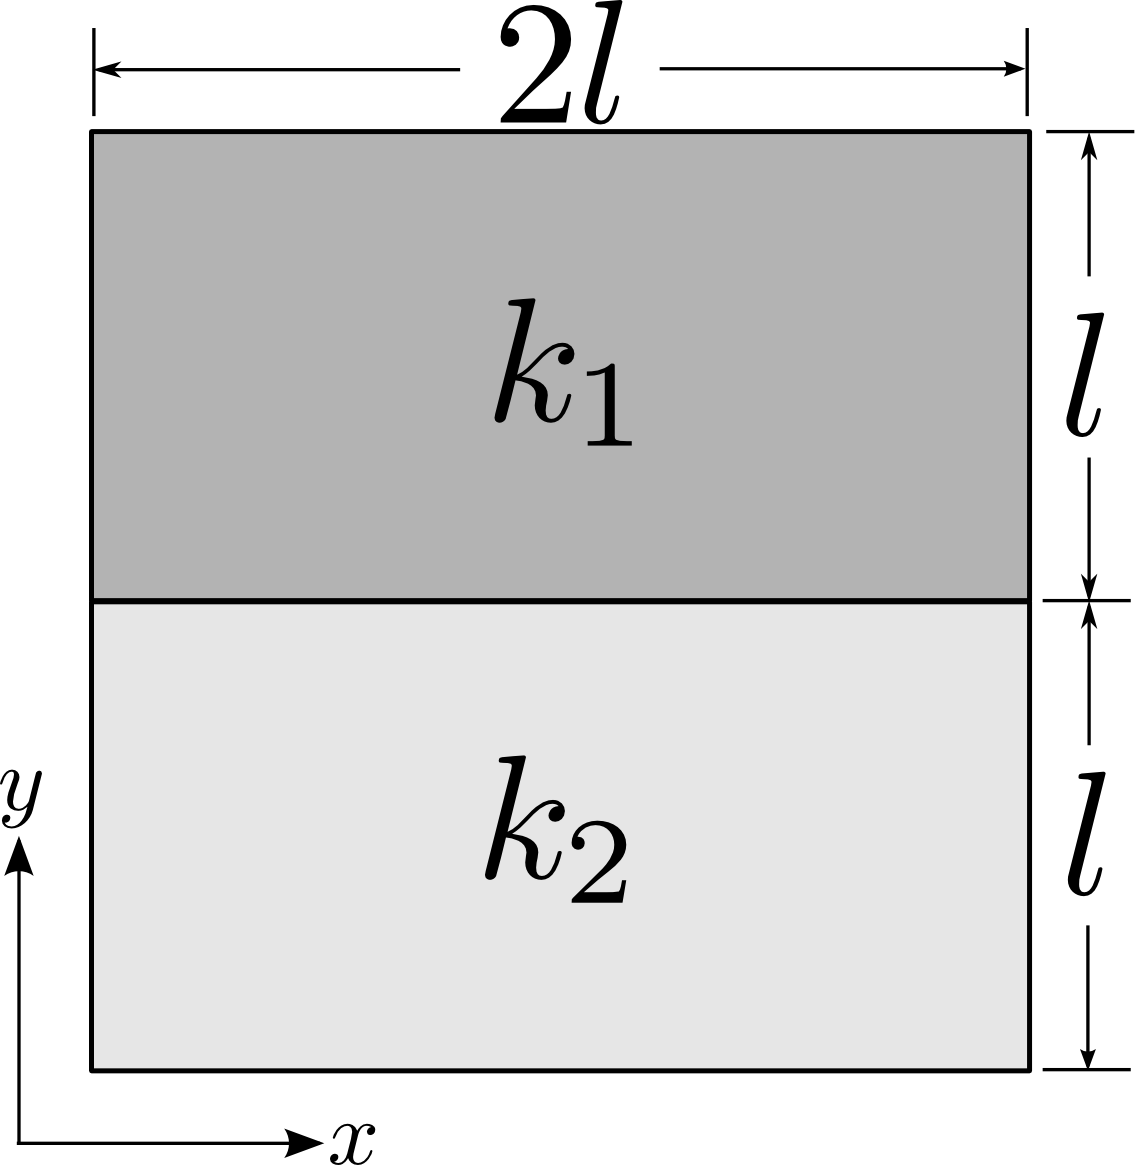
\includegraphics[width=0.3\textwidth]{fig/ex_laminate.png}
\label{fig:ex_laminate}
\caption{Two layers of materials create a different net conductivity value in the vertical direction than in the horizontal direction.}
\end{figure}

In the vertical direction, the effective thermal conductivity is
\(\frac12(k_1 + k_2)\). However, in the horizontal direction the effective
thermal conductivity is \(2\left( \frac1{k_1} + \frac1{k_2} \right)^{-1}\). An analogous analysis could be applied to a number of geometries.


\section{Measuring Anisotropic Thermal Conductivity}

This aggregate anisotropy brings a number of questions:

\begin{itemize}
\item Can anisotropic thermal conductivity in snow be measured with the needle
probe technique at all? If so, how accurately, and how many measurements would
one need?
\item How severe is anisotropy in snow? Is the amount of anisotropy
significant?
\item Is anisotropy in snow predictable? That is, could one take a single
measurement and extrapolate from it the anisotropic thermal conductivity?
\item Can anisotropy in snow explain historical differences between various
thermal conductivity measurements of snow using both the guarded hot plate and
needle probe techniques?
\end{itemize}

This document aims mostly to answer the first question. Developing a way
to measure anisotropic thermal conductivity with needle probes should enable
future researchers in answering the other questions. However, these other
questions will also, in part, be addressed.

\section{Anisotropic Model}

In every model studied, it has been assumed that the horizontal plane has the
same thermal conductivity and that only the vertical direction differs. In other
words, \(k_x = k_y = k_{xy} \ne k_z\). Each model aims to predict the measured
conductivity, \(k_{\textrm{meas}}\) as a function of angle.

In both analytical and numerical models and in the measurements, the angle
parameter, \(\theta\), is measured from the horizontal plane, as in Figure 
\ref{fig:angle}.

\begin{figure}[h]
\centering
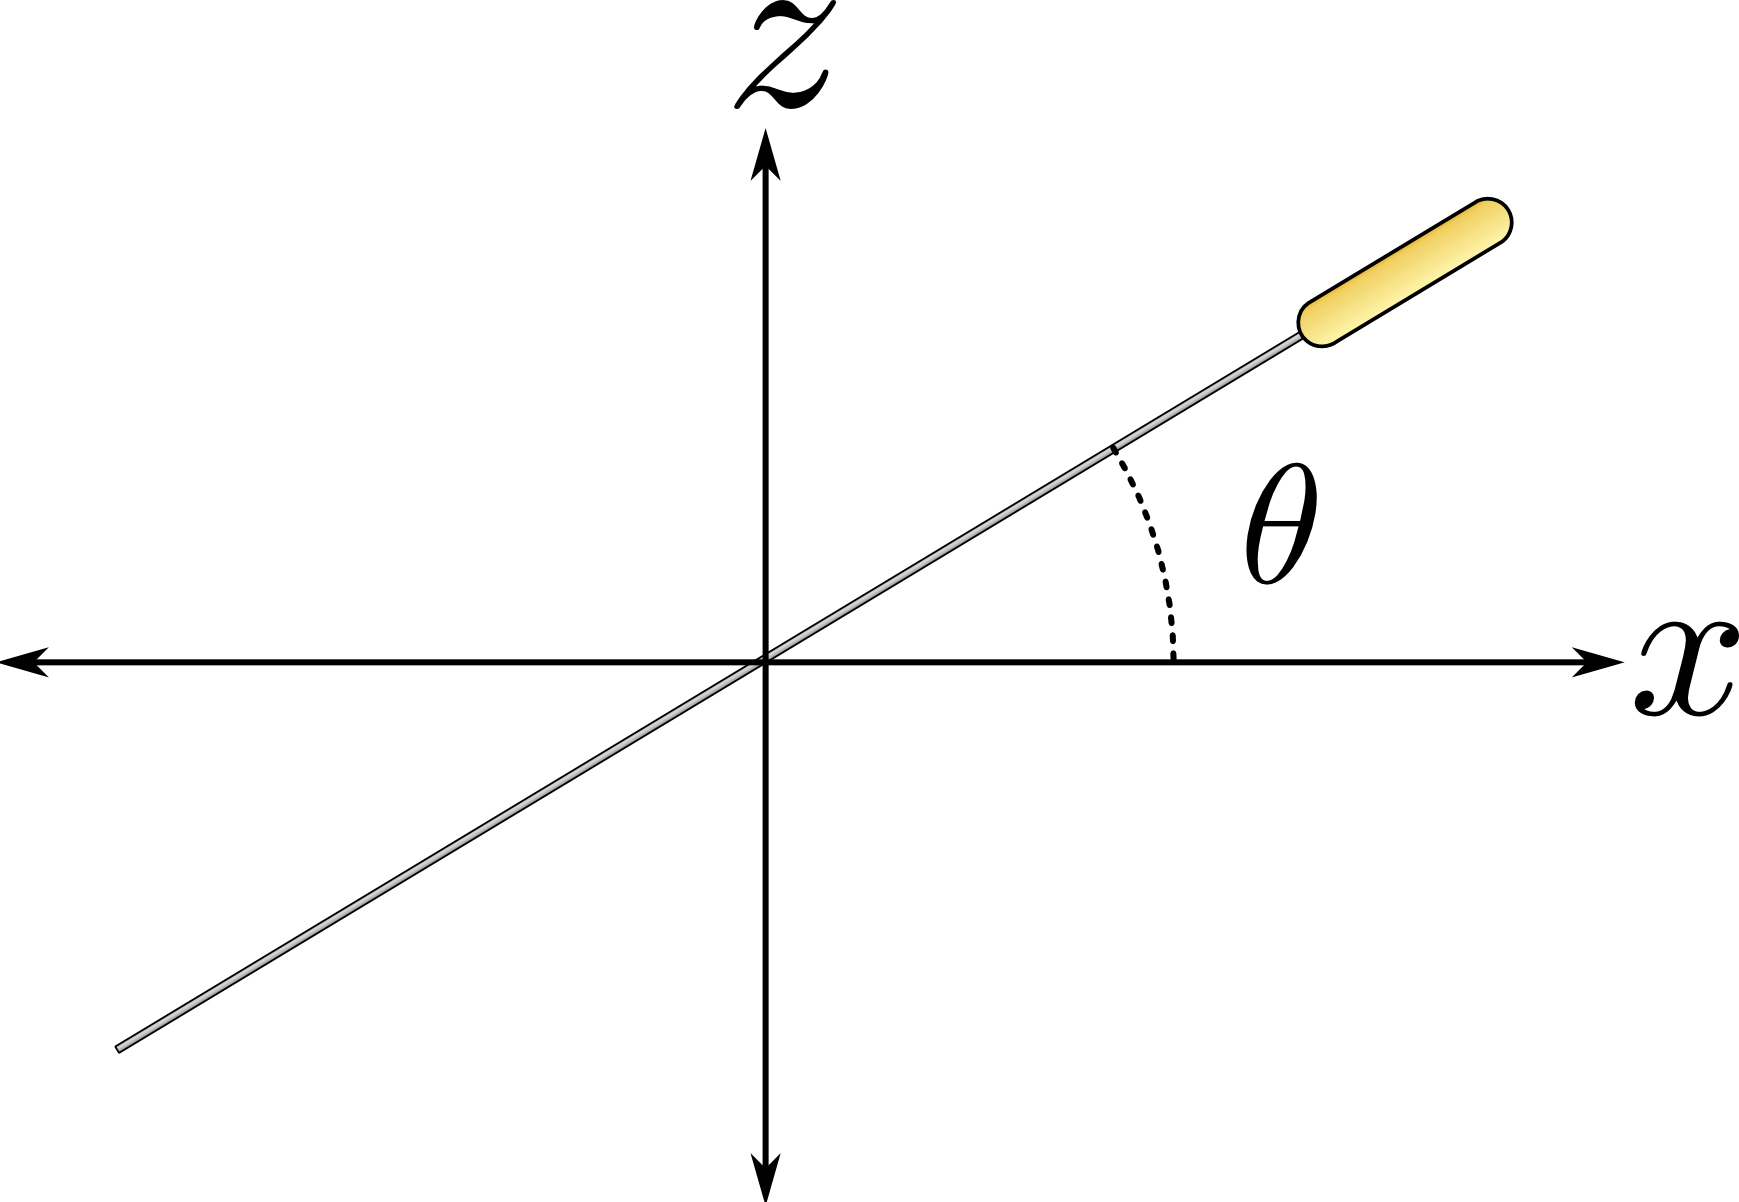
\includegraphics[width=0.3\textwidth]{fig/angle.png}
\label{fig:angle}
\caption{A diagram illustrating the measurement of angle in models and
measurements in this document. In all these cases, the angle is measured from
the horizontal plane, which is also the plane of isotropy. }
\end{figure}


\section{Document Outline}

First, this document will discuss the differential equations associated with
adapting the isotropic needle probe technique to the anisotropic case, as well
as analytical approaches to solving them. 

Second, the use of 3D finite element models in COMSOL with MATLAB to find 
numerical solutions to the problem will be discussed.

Then, this document will cover techniques for testing the predictions of the
these approaches with both real snow and engineered anisotropic materials, in
this case using table salt and table sugar.

The results of the analytical and numerical approaches will then be compared to
each other and the measurements of snow and engineered materials. The meanings
of these results are also discussed.

Finally, ``loose ends,'' unanswered questions, and avenues for future research
will be elucidated.

\chapter{Analytical Needle Probe Approach}
\label{sec:analytical-np}
\bigskip

\section{Introduction}

The technique used to measure thermal conductivity with a needle probe is based
on the assumption that the needle approximates an infinite line source of energy
with a constant heat flux embedded in an infinite medium. The origins of the
analytical solution for isotropic thermal conductivity may be found in Carslaw
and Jaeger's book, ``Conduction of Heat in Solids.'' \cite{basictheory}

The method based on Carslaw and Jaeger's solution depends on solving a 2-D
problem, where all planes orthogonal to the needle have the same temperature
distribution; in other words, temperature is not a function of axial position.
Moreover, the problem is further simplified by posing the problem into radial
coordinates and solving for temperature as a function of radial distance only.

In the isotropic case, this is straightforward, as conductivity is a constant
scalar. Unfortunately the anisotropic case is more complex, but luckily not
completely intractible.

\section{The Isotropic Case}

The isotropic case solves the following equation:

\begin{equation*}
k\nabla^2 T = \rho C\frac{\partial T}{\partial t}
\end{equation*}

Where \(T\) is temperature, \(k\) is a scalar thermal conductivity, \(\rho\) is
density, \(C\) is volumetric heat capacity, and \(t\) is time.

By casting this problem into cylindrical coordinates, the equations may be
simplified such that they are a function of radial distance \(r\) only (as
temperature is assumed to not be a function of axial position \(z\) or angle
\(\phi\)).

After applying this transformation and solving the equation, the analytical
solution to the problem becomes:

\begin{equation}
\label{isotropic_ei}
T(r,t) = - \frac{q}{4\pi k}\Ei\left(-\frac{r^2}{4kt}\right)
\end{equation}

where \(q\) is heat flux from the needle per linear distance, and \(\Ei()\) is
as defined in Equation \ref{eq:ei} for real-valued arguments.

\begin{equation}
\label{eq:ei}
\Ei(x) = -\int_{-x}^{\infty} \frac{e^{-t}}{t}dt
\end{equation}

Solving for the exponential integral analytically is not possible, and numerical
solutions can be difficult. Typically, an approximation for small
\(r^2/t\) is used instead:

\begin{equation}
\label{isotropic_case}
T(r,t) = \frac{q}{4\pi k}\ln\left(\frac{4kt}{r^2}\right) - \frac{\gamma q}{4\pi k}
\end{equation}

Typical use of this function is to find \(\frac{dT}{d(\ln t)}\) and solve
for \(k\). Equation \ref{isotropic_case} will be used for the remainder of
this analysis, though it could easily be applied to Equation \ref{isotropic_ei} as well.


\section{Difficulties in the Anisotropic Case}
\label{sec:analytical-np:anisotropic-diff}


The anisotropic case varies from the isotropic one in that instead of a scalar 
thermal conductivity \(k\), one must solve the problem using an \(n \times n\)
thermal conductivity, \([K]\), where \(n\) is the number of dimensions in the
problem. As a consequence, reducing the problem into two dimensions becomes more
difficult. Moreover, when the problem is posed in cylindrical coordinates, the
solution becomes a function not only of \(r\), but of \(\phi\) as well.

\section{Posing The Problem in Two Coordinates}
\label{sec:analytical-np:2D}

By assuming that temperature distribution is not a function of axial direction
\(z\), one may reduce the problem to an analogous one in orthogonal directions
\(x\) and \(y\) instead:

\begin{equation}
\nabla_{xy} \cdot \left([K]_{2 \times 2}\nabla_{xy} T \right)= \rho C\frac{\partial T}{\partial t}
\end{equation}

Without loss of generality, it may be further simplified like so:

\begin{equation}
\nabla \cdot \left(\begin{bmatrix}k_x & 0\\ 0 & k_y\end{bmatrix}\nabla T \right)= \rho C\frac{\partial T}{\partial t}
\end{equation}

This may be done by choosing the directions \(x\) and \(y\) such that the
matrix is diagonal.

The values of \(k_x\) and \(k_y\) may be found by finding the components of
\([K]\) that are in the \(xy\) plane.

%, as illustrated in \ref{fig:projection}. 
In particular, Equation \ref{eq:projection} was used in practice.

\begin{equation}
\label{eq:projection}
\left[ k_x, k_y \right] = 
\Eig\left(\begin{bmatrix} 1 & 0 & 0 \\ 0 & 1 & 0\\ 0 & 0 & 0\end{bmatrix}
\left[K\right]\right)
\end{equation}

\begin{comment}
\begin{figure}[h]
\centering
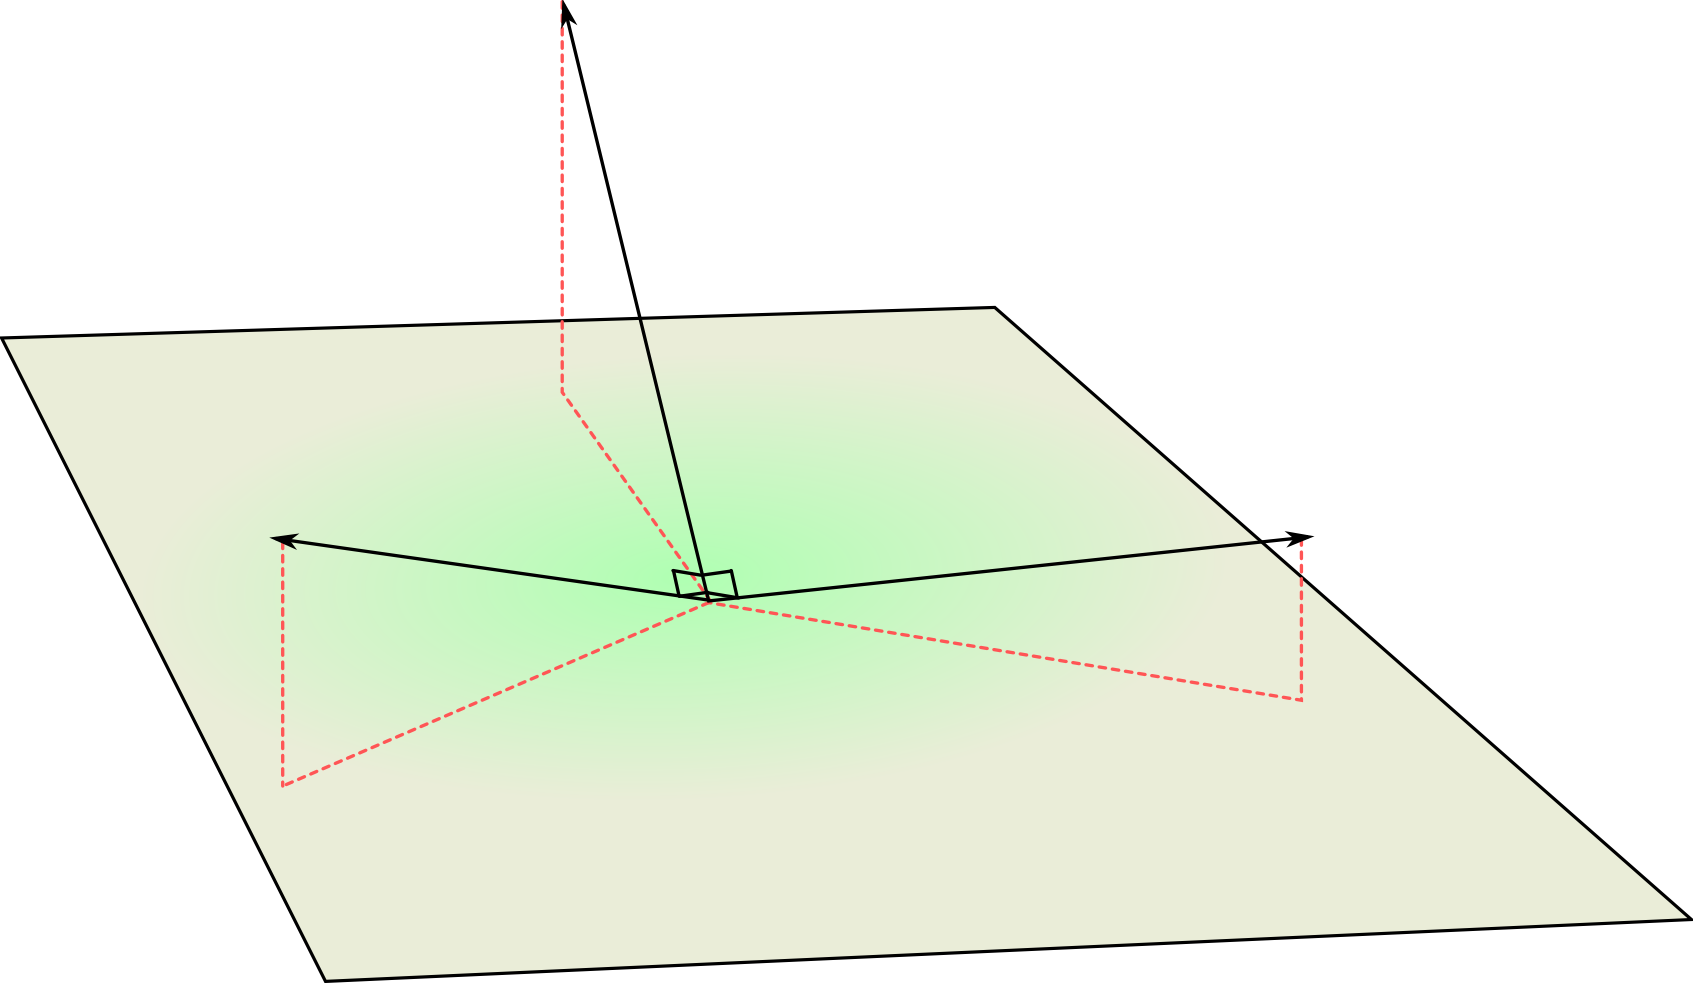
\includegraphics[width=0.6\textwidth]{fig/projection.png}
\label{fig:projection}
\caption{An informal demonstration of how the 3-D problem may be projected onto a 2-D domain.}
\end{figure}
\end{comment}

\section{Coordinate Transformation}
\label{sec:analytical-np:transformation}

\begin{figure}[h]
\centering
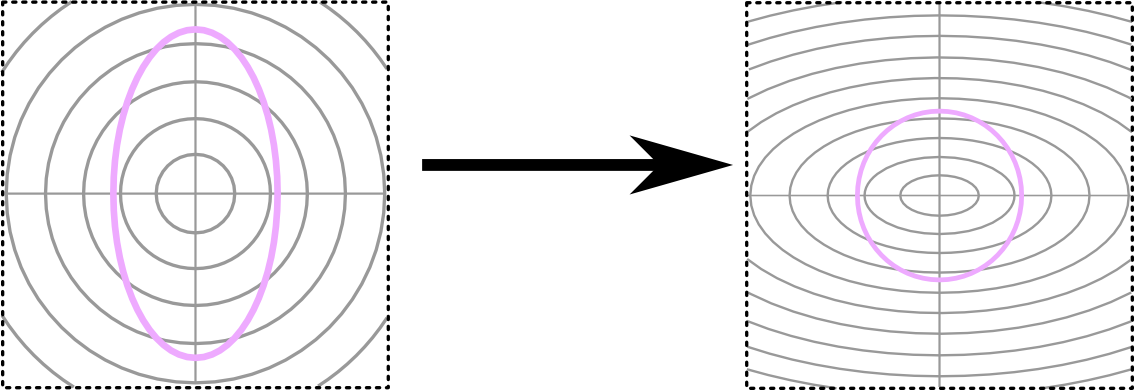
\includegraphics[width=0.8\textwidth]{fig/coordinate_transformation.png}
\caption{A 2-dimensional linear coordinate transformation.}
\label{fig:coord_trans}
\end{figure}

In order to apply the isotropic solution to this anisotropic case, a coordinate transformation may be applied such that the problem is transformed into
an isotropic case with respect to some \(x' = a_x x\) and \(y' = a_y y\), as in
Figure \ref{fig:coord_trans}.
Without loss of generality, suppose \(a_x = 1\).

\begin{align}
\frac{dx'}{dx} &= 1\\
\frac{dy'}{dy} &= a_y\\
\frac{\partial f}{\partial x} &= \frac{\partial f}{\partial x'}\frac{dx'}{dx} = \frac{\partial f}{\partial x'}\\
\frac{\partial f}{\partial y} &= \frac{\partial f}{\partial y'}\frac{dy'}{dy} = a_y\frac{\partial f}{\partial y'}\\
\nabla T &= \frac{\partial T}{\partial x'} \e_{x'} + a_y\frac{\partial T}{\partial y'} \e_{y'} \\
[K]\nabla T &= k_x\frac{\partial T}{\partial x'} \e_{x'} + k_ya_y\frac{\partial T}{\partial y'} \e_{y'}\\
\nabla \cdot \left([K]\nabla T\right) &= k_x\frac{\partial^2 T}{\partial {x'}^2} + k_ya_y^2\frac{\partial^2 T}{\partial {y'}^2}\\
\end{align}

Suppose the right hand side is equal to the equivalent isotropic expression:
\begin{equation}
k\left(\frac{\partial^2 T}{\partial {x'}^2} + \frac{\partial^2 T}{\partial {y'}^2} \right) = k_x\frac{\partial^2 T}{\partial {x'}^2} + k_ya_y^2\frac{\partial^2 T}{\partial {y'}^2}
\end{equation}

As a result,

\begin{align}
k &= k_x\\ a_y &= \sqrt{\frac{k_x}{k_y}}\\
\end{align}

Therefore, the following coordinate transformation will allow for the application
of isotropic solutions to an isotropic case with \(k = k_x\):

\begin{equation}
    \label{coord_trans}
    \begin{pmatrix}x' \\ y'\end{pmatrix} =
    \begin{bmatrix}1 & 0\\ 0 & \sqrt{\frac{k_x}{k_y}} \end{bmatrix}\begin{pmatrix}x \\ y\end{pmatrix}
\end{equation}

\section{From Temperature Distribution to Effective Thermal Conductivity}

Using Equation \ref{coord_trans}, the isotropic solution may be applied:

\begin{equation}
    k_x \nabla^2 T = \rho C\frac{\partial T}{\partial t}
\end{equation}

to yield the following result (for sufficiently large \(t/(r')^2\)):

\begin{equation}
T(r',t) = \frac{q}{4\pi k_x}\ln\left(\frac{4k_xt}{r'^2}\right) - \frac{\gamma q}{4\pi k_x}
\end{equation}

In the isotropic case, the value of \(r\) does not change the derivative with
respect to the natural log of time, as long as it is assumed constant. In contrast, the anisotropic case requires that another transformation is applied
to \(r'\) so that both \(k_x\) and \(k_y\) may be recovered. This requires that
some contextual meaning is assigned to \(r\) and \(r'\). In this analysis, it
is assumed that the measurement occurs at some  \(r = r_{\textrm{0}}\), perhaps
on the surface of the physical needle.

This approach isn't without its problems. For example, it supposes that the
isotherms are all circles in the transformed geometry, but if a finite-sized
needle was actually being modeled in the problem then the isotherms near the
(elliptically-shaped in the transformed domain) needle would be elliptical as
well, and only isotherms sufficiently far away would be round. However, this
approach allows us to keep using the \(\ln()\) approximation, while a solution
given a finite needle would likely require the use of Bessel functions.

Applying this technique to the anisotropic case, \(r_{xy} = \cos(\theta) \hat{e}_x + \sin(\theta) \hat{e}_y \) must also be transformed
into \(r_{x'y'}\):

\begin{align*}
    \begin{pmatrix}r_{x'} \\ r_{y'}\end{pmatrix} &=
    \begin{bmatrix}1 & 0\\ 0 & \sqrt{\frac{k_x}{k_y}} \end{bmatrix}\begin{pmatrix}r_0\cos(\theta) \\ r_0\sin(\theta)\end{pmatrix}\\
    &= r_0\left(\cos(\theta) \e_x + \sqrt{\frac{k_x}{k_y}} \e_y \right)\\
\end{align*}
\begin{equation}
    \norm{r'}^2 = r_0^2 \left(\cos^2(\theta) + \frac{k_x}{k_y}\sin^2(\theta) \right)\\
\end{equation}

This means that the temperature around the needle should now vary as a function
of \(\theta\), unlike in the isotropic case. Now, since the needle only measures
a single value, it may be assumed that the measured quantity is an
average temperature, such as the average surface temperature of the probe.  This
may be expressed like so:

\begin{equation}
\label{eq:tavg}
T_{\textrm{avg}}(t) = \frac{4\pi k_x}{q} \frac{\mathcal{E}(\ln(t), \frac{k_x}{k_y})}{\mathcal{E}(1, \frac{k_x}{k_y})}
\end{equation}

\hspace{-\parindent}where:

\begin{equation}
\mathcal{E}(f(\phi, \alpha), \alpha) = \int_0^{2\pi} f\sqrt{\cos^2(\phi) + \alpha\sin^2(\phi)} d\phi
\end{equation}

\section{Finding Effective Conductivity as a Function of Needle Orientation}

In order to extract the effective \(k\) value, a function of the form
\(C_1 \ln(t) + C_2\) is fit to Equation \ref{eq:tavg}. Then, all that is left is to evaluate the functions at various combinations of
\(k_xy\), \(k_z\) and \(\theta\).

\section{Conclusions}
\label{sec:analytical-np:conclusion}

An analytical approach to studying anisotropic thermal conductivity with needle
probes is more difficult than with the isotropic case. However, by using
coordinate projections to pose the problem in two dimensions, and by applying
coordinate transformations to the domain, one may apply the accepted isotropic
theory to the anisotropic case with minimal modification.  By numerically
evaluating the predicted temperature distribution over time, one may find the
expected conductivity measurement given the theory holds for anisotropic
materials.


\chapter{Numerical Needle Probe Approach}
\label{sec:numerical-np}
\bigskip

\section{Introduction} 
\label{sec:numerical-np:introduction}

Numerical experiments simulated needle probes in anisotropic mediums with
three-dimensional finite element heat transfer models in COMSOL 3.5a. While the
models themselves were relatively simple, attempting to automate a parameter
study in COMSOL 3.5a with respect to the anisotropic material properties proved
difficult.

\section{Geometry and Domain Properties}
\label{sec:numerical-np:domain}

\begin{table}[h]
\label{tab:constants}
\centering
\caption{Constants Used in Numerical Models}
\begin{tabular}{r | l}
radius of needle & \(0.25\) mm\\
length of needle & \(10\) cm\\
radius of snow & \(40\) cm\\
\hline
density of needle & \(8000\) kg/\(\textrm{m}^3\)\\
\(C_P\) of needle & \(460\) \textbf{*units*}\\
\(q\) of needle & \(0.5\) W/m\\
\(k\) of needle & \(160\) \textbf{*units*}\\
\hline
density of snow & \(200\) kg/\(\textrm{m}^3\)\\
\(C_P\) of snow & \(2050\) \textbf{*units*}
\end{tabular}
\end{table}

The needle was simulated as a long, thin steel cylinder embedded in the center
of a sphere of snow. While most of the dimensions and material properties were
held constant (see Table \ref{tab:constants}), the anisotropic conductivity of
the snow was parameterized in the form of a \(3\times3\) symmetric, positive
definite matrix.  In practice, this was done by specifying a diagonal matrix
\(\Lambda\) with positive eigenvalues \(k_{xy}\) and \(k_z\) and a rotation
matrix \(R\) around the \(x\) axis, and then defining \(K = R^T\Lambda R\) as in
equation \ref{eq:rotdiagrot} :

\begin{equation}
\label{eq:rotdiagrot}
K = \begin{bmatrix}
\cos(\theta) & 0 & \sin(\theta)\\
0 & 1 & 0\\
-\sin(\theta) & 0 &\cos(\theta)
\end{bmatrix}
\begin{bmatrix}
k_{xy} & 0 & 0\\
0 & k_{xy} & 0\\
0 & 0 & k_z
\end{bmatrix}
\begin{bmatrix}
\cos(\theta) & 0 & \sin(\theta)\\
0 & 1 & 0\\
-\sin(\theta) & 0 &\cos(\theta)
\end{bmatrix}
\end{equation}

The boundary conditions on the surface of the sphere enforced zero heat flux,
and the radius of the sphere was chosen such that the sphere approximated an
infinite medium.

Point temperatures recorded were the center of the needle, which corresponds to
the location of the thermocouple used in real-world experiments, and six points
on the surface of the snow, to ensure that the sphere was sufficiently large.

\section{MATLAB in Geometry-Based Parameter Studies Using COMSOL 3.5a}
\label{sec:numerical-np:matlab}

Unfortunately, COMSOL 3.5a did not have the facilities necessary to implement a
geometry-changing multi-parameter study as required from the GUI alone. However,
COMSOL 3.5a did have facilities for scripting with MATLAB. Unfortunately, I
found the facility to be poorly-documented, and, at least with the particular
install hosted by ARSC, buggy and prone to crashing.

MATLAB code written to implement the parameter study was largely auto-generated
by COMSOL, by building a base model in COMSOL 3.5a and exporting to an m-file.
This code was then split into two parts: The meshing code, and the solving code.
These pieces of code were wrapped in functions, called ``mesher'' and ``solver''
respectively, and used by a main procedure called ``worker.m.'' Contained in
``worker.m'' is a MATLAB structure with the constants outlined in section
\ref{sec:numerical-np:domain} called ``params'':

\small
\begin{minted}{matlab}
    params=struct('rsnow', 0.4, ...
                  'rneedle', 0.00025, ...
                  'lneedle', 0.1, ...
                  'density_snow', 200, ...
                  'density_needle', 8000, ...
                  'cp_snow', 2050, ...
                  'cp_needle', 460, ...
                  'q_needle', 0.5, ...
                  'k_needle', 160, ...
                  'time', [logspace(0.1,1,15) logspace(1,3,15)], ...
                  'angles', angles );
\end{minted}
\normalsize

This structure also contains a list of angles yet to be solved for, and the
times for which to solve.

The meshing code was wrapped in a function called ``mesher'' and took an angle
(in degrees) and the params structure as arguments, and is for the most part
simply code generated by COMSOL:

%% MESHER %%%%%%%%%%%%%%%%%%%%%%%%%%%%%%%%%%%%%
\small
\begin{minted}{matlab}

% COMSOL Multiphysics Model M-file
% Generated in part by COMSOL 3.5a (COMSOL 3.5.0.608, $Date: 2009/05/11 07:38:49 $)
% the rest of it modified by Joshua Holbrook

function fem=mesher(angle,params)
    % mesh_generate(angle)
    % generates a mesh for the given angle. 

    fprintf(['meshing for angle=' num2str(angle) '...\n']);

    flclear fem

    % COMSOL version
    clear vrsn
    vrsn.name = 'COMSOL 3.5';
    vrsn.ext = 'a';
    vrsn.major = 0;
    vrsn.build = 608;
    vrsn.rcs = '$Name: v35ap $';
    vrsn.date = '$Date: 2009/05/11 07:38:49 $';
    fem.version = vrsn;
\end{minted}
\normalsize

The COMSOL code was changed to use the arguments passed to ``mesher'' instead of
the values used in the original model:

\small
\begin{minted}{matlab}
    % Geometry
    g1=sphere3(num2str(params.rsnow),'pos',{'0','0','0'},'axis',{'0','0','1'},'rot','0');
    g2=cylinder3(num2str(params.rneedle),num2str(params.lneedle),'pos',{num2str(-params.lneedle/2),'0','0'},'axis',{'1','0','0'},'rot','0');
    parr={point3(0,0,0)};
    g3=geomcoerce('point',parr);
    parr={point3(params.rsnow,0,0)};
    g4=geomcoerce('point',parr);
    parr={point3(0,params.rsnow,0)};
    g5=geomcoerce('point',parr);
    parr={point3(0,0,params.rsnow)};
    g6=geomcoerce('point',parr);
    parr={point3(-params.rsnow,0,0)};
    g7=geomcoerce('point',parr);
    parr={point3(0,-params.rsnow,0)};
    g8=geomcoerce('point',parr);
    parr={point3(0,0,-params.rsnow)};
    g9=geomcoerce('point',parr);
\end{minted}
\normalsize

Here, it can be seen that a number of points are generated: First, the point
representing the thermocouple temperature at \((0, 0, 0)\), and then six points
over the surface of the sphere.

Notice that, in this code, ``theta'' is never actually used. This is
because, in early iterations of the code, the needle was rotated by the angle
``theta.'' However, this seemed to cause random errors from COMSOL's meshing
procedures, so the anisotropic thermal properties of the snow were changed
instead, as outlined in section \ref{sec:numerical-np:domain}. However, the
argument was retained in order to avoid editing other legacy code in the model.

Afterwards, geometry is labelled and a mesh is initialized and refined using
code generated by COMSOL, and returns the COMSOL ``fem'' structure:

\small
\begin{minted}{matlab}

    % Analyzed Geometry
    clear p s
    p.objs={g3,g4,g5,g6,g7,g8,g9};
    p.name={'ORIGIN','PT1','PT2','PT3','PT4','PT5','PT6'};
    p.tags={'g3','g4','g5','g6','g7','g8','g9'};

    s.objs={g1,g2};
    s.name={'SNOW','NEEDLE'};
    s.tags={'g1','g2'};

    fem.draw=struct('p',p,'s',s);
    fem.geom=geomcsg(fem);


    % ODE Settings
    clear ode
    clear units;
    units.basesystem = 'SI';
    ode.units = units;
    fem.ode=ode;


    % Initialize mesh
    fem.mesh=meshinit(fem, ...
                      'hauto',5, ...
                      'hgradsub',[2,1.1], ...
                      'hmaxsub',[2,0.0005]);

    % Refine mesh
    fem.mesh=meshrefine(fem, ...
                        'mcase',0, ...
                        'rmethod','longest');

    fem=multiphysics(fem);
end
\end{minted}
\normalsize

This ``fem'' structure may then be passed to the ``solver'' function, along
with parameters describing the snow's material properties and the needle's
orientation with respect to the snow. Similarly, the ``solver'' function is
mostly COMSOL code wrapped in a function:

\small
\begin{minted}{matlab}
% COMSOL Multiphysics Model M-file
% Generated by COMSOL 3.5a (COMSOL 3.5.0.608, $Date: 2009/05/11 07:38:49 $)
% the rest of it modified by Joshua Holbrook

function answer=solver(kxy,kz,fem,theta,params)
    %solver(kxy,kz,mesh,theta,params)
    %uses comsol to pump out a solution using a given mesh-mat and a k-matrix in comsol format.

    fprintf(['solving for kxy=' num2str(kxy) ' and kz=' num2str(kz) '...\n']);
    % Application mode 1
    clear appl
    appl.mode.class = 'GeneralHeat';
    appl.module = 'HT';
    appl.shape = {'shlag(1,''J'')','shlag(2,''T'')'};
    appl.sshape = 2;
    appl.assignsuffix = '_htgh';
    clear bnd
    bnd.type = {'q0','cont'};
    bnd.shape = 1;
    bnd.ind = [1,1,1,1,2,2,2,2,2,1,1,1,1,2];
    appl.bnd = bnd;
    clear equ
    equ.sdtype = 'gls';
\end{minted}
\normalsize

Here, parameters or the material properties are attached to the domain:

\small
\begin{minted}{matlab}
    % densities
    equ.rho = {params.density_snow,params.density_needle};
    equ.init = 0;
    equ.shape = 2;
    % Heat capacities
    equ.C = {params.cp_snow,params.cp_needle};
    % Wattage
    equ.Q = {0,params.q_needle/pi/(params.rneedle)^2};
    % Heat conductivities
    arr = [cos(theta*pi/180), 0, sin(theta*pi/180); 0, 1, 0; -sin(theta*pi/180), 0, cos(theta*pi/180)]; %rotation matrix
    equ.k = {symmetric_tocell(arr*diag([kxy,kxy,kz])*(arr')),params.k_needle};
\end{minted}
\normalsize

This is also where the symmetric matrix is generated, as described in section
\ref{sec:numerical-np:domain}. ``symmetric\_tocell'' is a helper function which
converts symmetric matrices of the form 
\minted{matlab}{[a1 a2 a4; a2 a3 a5; a4 a5 a6]} to the form
\minted{matlab}{ {a1, a2, a3, a4, a5, a6 }}.

Then, more code generated by COMSOL:

\small
\begin{minted}{matlab}
    equ.ind = [1,2];
    appl.equ = equ;
    fem.appl{1} = appl;
    fem.frame = {'ref'};
    fem.border = 1;
    fem.outform = 'general';
    clear units;
    units.basesystem = 'SI';
    fem.units = units;

    % Coupling variable elements
    clear elemcpl
    % Integration coupling variables
    clear elem
    elem.elem = 'elcplscalar';
    elem.g = {'1'};
    src = cell(1,1);
    clear bnd
    bnd.expr = {{'T',{}},{'1',{}}};
    bnd.ipoints = {{'4',{}},{'4',{}}};
    bnd.frame = {{'ref',{}},{'ref',{}}};
    bnd.ind = {{'1','2','3','4','10','11','12','13'},{'5','6','7','8','9', ...
      '14'}};
    src{1} = {{},{},bnd,{}};
    elem.src = src;
    geomdim = cell(1,1);
    geomdim{1} = {};
    elem.geomdim = geomdim;
    elem.var = {'int_T','area'};
    elem.global = {'1','2'};
    elemcpl{1} = elem;
    fem.elemcpl = elemcpl;

    % ODE Settings
    clear ode
    clear units;
    units.basesystem = 'SI';
    ode.units = units;
    fem.ode=ode;

    % Multiphysics
    fem=multiphysics(fem);

    % Generate GMG mesh cases
    fem=meshcaseadd(fem,'mgauto','anyshape');

    % Extend mesh
    fem.xmesh=meshextend(fem);

    % Solve problem
    fem.sol=femtime(fem, ...
                    'solcomp',{'T'}, ...
                    'outcomp',{'T'}, ...
                    'blocksize','auto', ...
                    'tlist', params.time, ...
                    'estrat',1, ...
                    'tout','tlist', ...
                    'linsolver','gmres', ...
                    'itrestart',100, ...
                    'prefuntype','right', ...
                    'prefun','gmg', ...
                    'prepar',{'presmooth','ssor','presmoothpar',{'iter',3,'relax',0.8},'postsmooth','ssor','postsmoothpar',{'iter',3,'relax',0.8},'csolver','pardiso'}, ...
                    'stopcond','0.06-int_T/area', ...
                    'mcase',[0 1]);

    % Save current fem structure for restart purposes
    fem0=fem;
\end{minted}
\normalsize

Code to plot the solution was commented out and replaced with code to save the
temperature data at the center of the needle, and the average temperature of the
six points at the surface of the sphere, to MATLAB variables:

\small
\begin{minted}{matlab}

    % Plot solution
    %{
    postplot(fem, ...
             'slicedata',{'T','cont','internal','unit','K'}, ...
             'slicexspacing',5, ...
             'sliceyspacing',0, ...
             'slicezspacing',0, ...
             'slicemap','Rainbow', ...
             'solnum','end', ...
             'title','Time=100    Slice: Temperature [K]', ...
             'grid','on', ...
             'campos',[-2.636014311828346,-3.4353207343472505,2.4999999999999996], ...
             'camtarget',[0,0,0], ...
             'camup',[0,0,1], ...
             'camva',41.213465344831754);
    %}

    % Integrate
    T_thermistor=postint(fem,'T', ...
               'unit','K', ...
               'recover','off', ...
               'dl',8, ...
               'edim',0, ...
               'solnum','all');

    % Integrate
    T_surf_avg=postint(fem,'T', ...
               'unit','', ...
               'recover','off', ...
               'dl',[1,2,3,4,10,11,12,13], ...
               'edim',2, ...
               'solnum','end');
\end{minted}
\normalsize

Finally, the data is packed into a cell array, and the ``angles'' parameter
is changed:

\small
\begin{minted}{matlab}

    answer={[fem.sol.tlist; T_thermistor],T_surf_avg};
    angles = params.angles(2:length(params.angles));

    %flsave(['fem-' num2str(theta) '-' num2str(kxy) '-' num2str(kz) '.mph']);

    save('angles.m', 'angles');
end
\end{minted}
\normalsize

In some runs, the fem structure was exported back to the COMSOL format for
further study.

\section{Automatic Calculation of Conductivity from Simulated Time/Temperature Data}

Results from COMSOL were automatically fitted against the linear model with
respect to \(\ln(t)\) by ``dropping'' early \((t,T)\) datapoints until the
correlation coefficient of the remaining points was sufficiently high. Then, a
linear curvefit was applied to these remaining points. Finally, the slope was
used to calculate \(k_{\textrm{meas}}\).

\small
\begin{minted}{matlab}
function k = fitter(t,T,rset,params)
    logt = log(t(t>1));
    T = T(t>1);

    disp('Finding linear portion...');    
    for i=1:length(logt)-1
        C = corrcoef(logt(i:length(logt)), T(i:length(T)));
        r = sqrt(C(2,1));
        if r > rset %adjust this to get 'good' values
            disp([ 'linear fitting to ' ...
                   num2str((length(logt)-i)) ...
                   ' points from t=' num2str(exp(logt(i))) ...
                   ' to t=' ...
                   num2str(exp(logt(length(logt)))) ...
                   '...']);
            x = polyfit(logt(i:length(logt)),T(i:length(T)), 1);
            break
        end
    end

    k = (params.q_needle)/(4*pi*x(1));
end
\end{minted}
\normalsize

\section{Organization and Serialization of Results}

Simulation results were saved in a .mat file, which is MATLAB's native
serialization format. Results were organized into a nested cell array which
mirrored the format of two MATLAB matrices k\_xy and k\_z:

These functions were called by ``worker.m,'' which was used to run multiple
tests and save the results.

%% WORKER %%%%%%%%%%%%%%%%%%%%%%%%%%%%%%%%%%%%%
\small
\begin{minted}{matlab}
%worker.m
%does the working

function worker(kxy,kz)
    load('angles.mat', 'angles');
    angles
    [kxy,kz] = meshgrid(kxy,kz);

    %flreport('off');

    params=struct('rsnow', 0.4, ...
                  'rneedle', 0.00025, ...
                  'lneedle', 0.1, ...
                  'density_snow', 200, ...
                  'density_needle', 8000, ...
                  'cp_snow', 2050, ...
                  'cp_needle', 460, ...
                  'q_needle', 0.5, ...
                  'k_needle', 160, ...
                  'time', [logspace(0.1,1,15) logspace(1,3,15)], ...
                  'angles', angles );

    saveroot=['./solutions-' date '/'];

    mesh = mesher(0,params);
    for angle=angles,
        try
            solutions = arrayfun(@(x,y) solver(x,y,mesh,angle,params), ...
                            kxy,kz, 'UniformOutput', false);
            save solutions
            fprintf('Fitting solutions...\n');
            solutions = {cellfun(@(tsd) {fitter(tsd{1}(1,:),tsd{1}(2,:), ...
                                             0.999,params), ...
                             tsd{1}, tsd{2}}, ...
                         solutions, 'UniformOutput', false)};
            fprintf('A solution set just completed.');
            system([ 'echo "A solution set finished on" `hostname` ' ...
                     '| mutt -s "A solution set completed." ' ...
                     'josh.holbrook@gmail.com' ]);
        catch exception
            system([ 'echo "Exception occurred on" `hostname` ' ...
                     '| mutt -s "Exception occurred--' exception.message ...
                     '" josh.holbrook@gmail.com' ]);
        end
        angles = angles(2:length(angles));
        save('angles.mat', 'angles');
        %solutions
        mkdir(saveroot);
        save([ saveroot 'solution-' num2str(angle) ], ...
             'solutions','angle','kxy','kz','params');
    end

    % Emails me when everything's done
    system([ 'echo "Results completed on " `hostname` ' ...
             '| mutt -s "Results Completed" ' ...
             'josh.holbrook@gmail.com' ]);
    system('touch down');
end
\end{minted}
\normalsize
%%%%%%%%%%%%%%%%%%%%%%%%%%%%%%%%%%%%%

The data stored in each slot of the nested array was itself a cell array
containing the simulation results, as shown in figure \ref{fig:cellarray}:

% Bastardization of tabular use.
\begin{figure}
\label{fig:cellarray}

\centering
\begin{tabular}{| c | c | c |}
\hline
\(k_\textrm{meas}\) & \( \left[ \textrm{time}, \textrm{temperature} \right]^T\) & Average surface temperature of sphere\\
\hline
\end{tabular}
\caption{Contents of the cell array.}
\end{figure}

\section{Post-Simulation Analysis with MATLAB}

\section{Code Architecture and Use}

% \section{Verification with Analytical Approach}

\chapter{Experimental Measurements}
\label{sec:irl}

\section{Introduction}

In addition to theoretical results, real world cases must be measured
in order to validate the theory. In this chapter, methods for making actual
measurements in both snow and in engineered materials are explored. Moreover,
methods for building engineered materials are discussed.


\section{Needle Probe Measurement Fundamentals}

Needle probe measurements are taken using an apparatus borrowed from the Cold
Regions Research and Engineering Laboratory (CRREL), illustrated in Figure
\ref{fig:apparatus}. Encased in a Pelican case for protection are a Campbell
CR10X data logger, a relay switch, a 12v gel cell for the CR10X and a series of
D-cells to power the heating coils in the needle. The program that came with the
data logger uses the relay switch to control the heat flux from the needle, and
records temperature data from the needle's thermocouple, as well as the voltage
across the heating element, over the course of a five minute heating curve and
a ten minute cooling curve.

\begin{figure}[h]
\centering
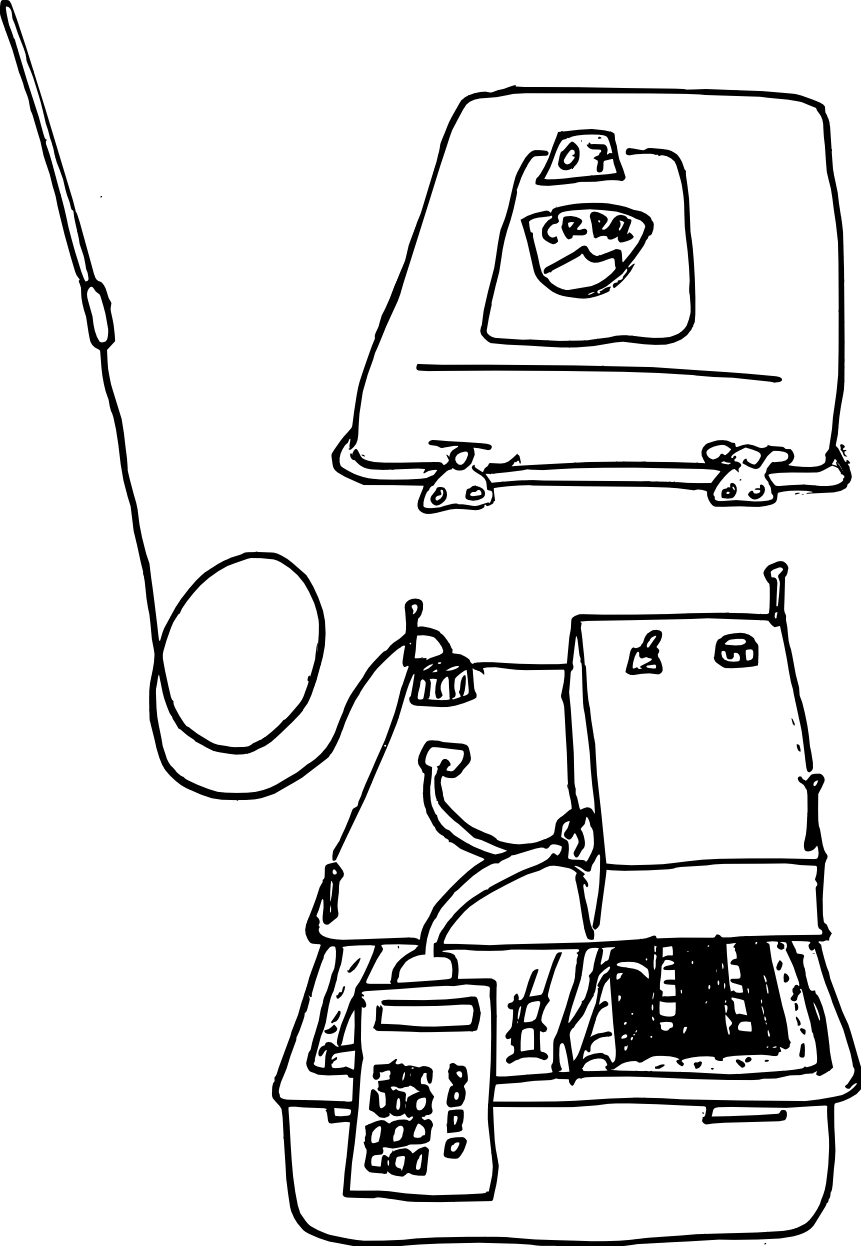
\includegraphics[width=0.7\textwidth]{fig/apparatus.png}
\caption{Extruded illustration of the needle probe apparatus. Major parts are labelled.}
\label{fig:apparatus}
\end{figure}

Once testing is complete, data may be uploaded from the data logger using
Campbell's PC200W software (shown in Figure \ref{fig:pc200w}) and a serial connection.

\begin{comment}
\begin{figure}[h]
\centering
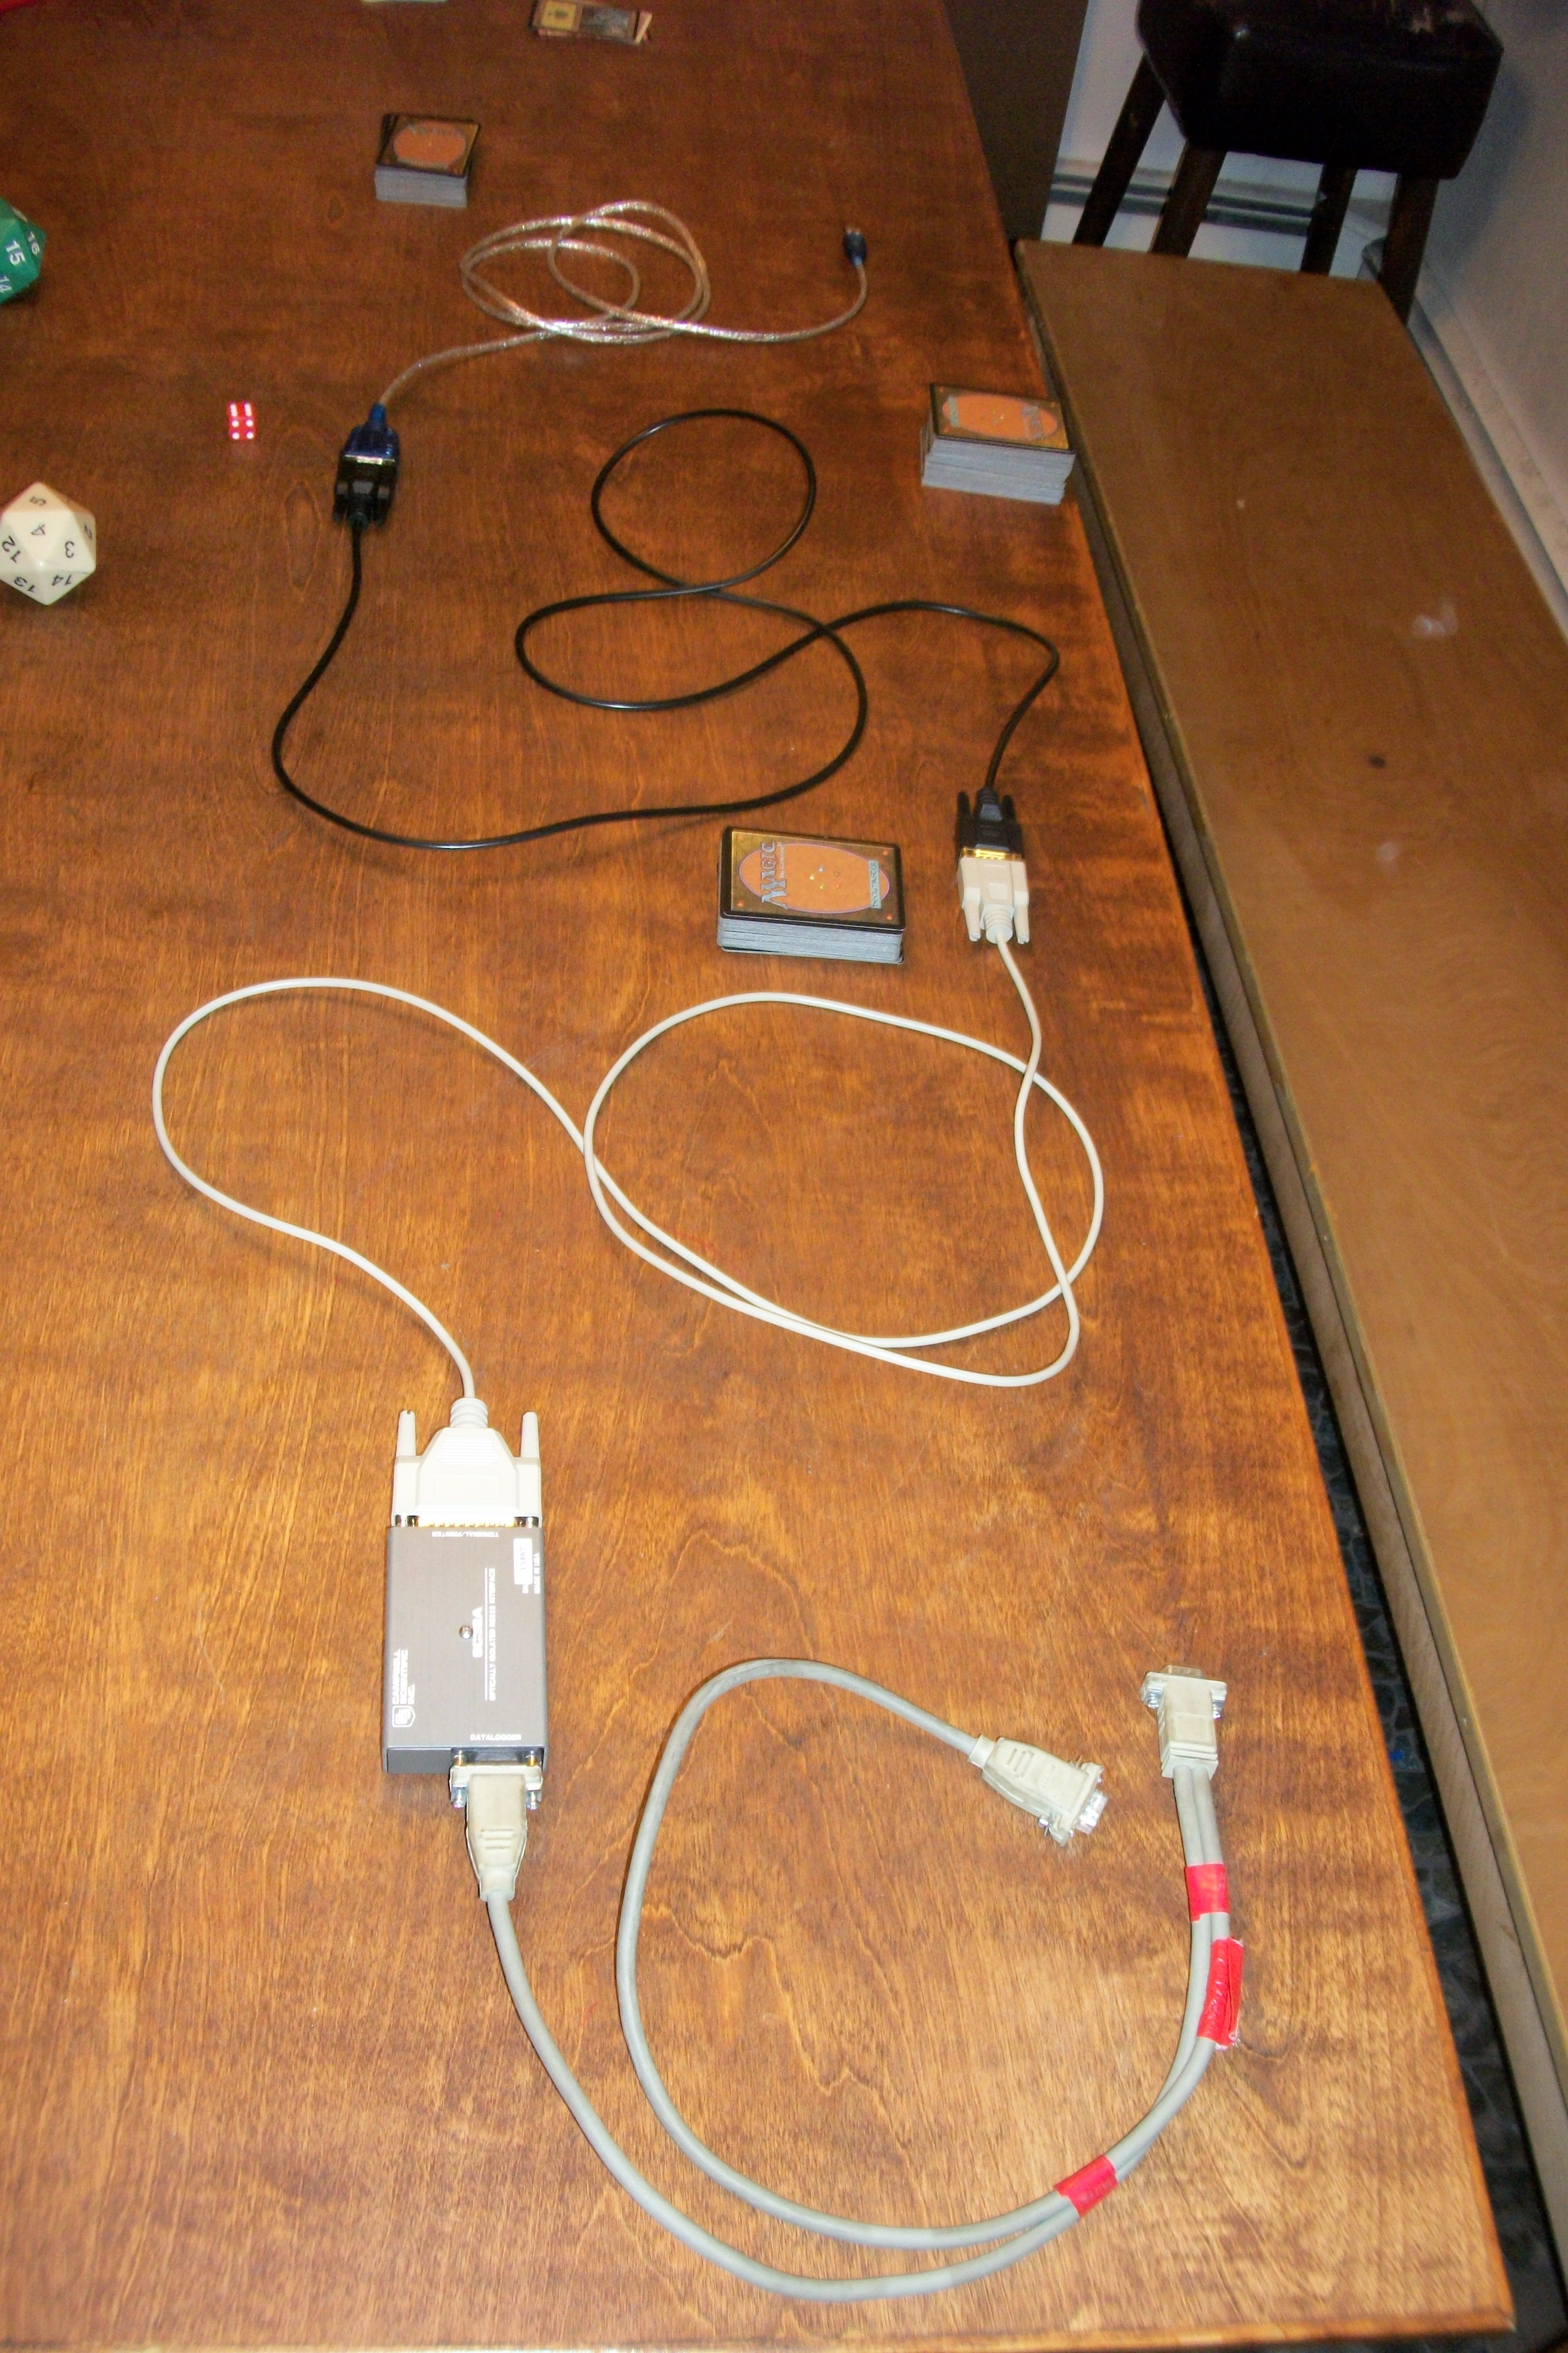
\includegraphics[width=0.6\textwidth]{fig/cable.jpg}
\caption{The cables used to communicate with the datalogger.}
\label{fig:cable}
\end{figure}
\end{comment}

Using PC200W, data may be uploaded from the CR10X in a raw binary format and then
converted to a .csv format. This .csv data may be analyzed with either spreadsheet software, a series of
scripts, or both. For this series of experiments, Excel, Gnumeric and cat/append are used
to verify the existence of data and to combine datasets, while python is used
for the analysis.  Generally, each analysis consists of subtracting \(t_0\)
from the relevant time intervals, subsetting the collected data over a straight
section, and finding the slope.  In addition, a correction factor, named the
McGaw Cooling Curve Correction after a CRREL researcher, is used for benchtop
measurements to account for the insulation around the apparatus.

Generally, each measurement also has some metadata associated with it. In
particular, anisotropic measurements have an angle associated with them, and
snow measurements also have a coordinate position on the snowpack associated
with them. These are measured with a protractor and a tape measure,
respectively. This means that, while taking measurements, one has to be careful
to make sure that they can keep the proper metadata associated with each
measurement.

\begin{figure}[h]
\centering
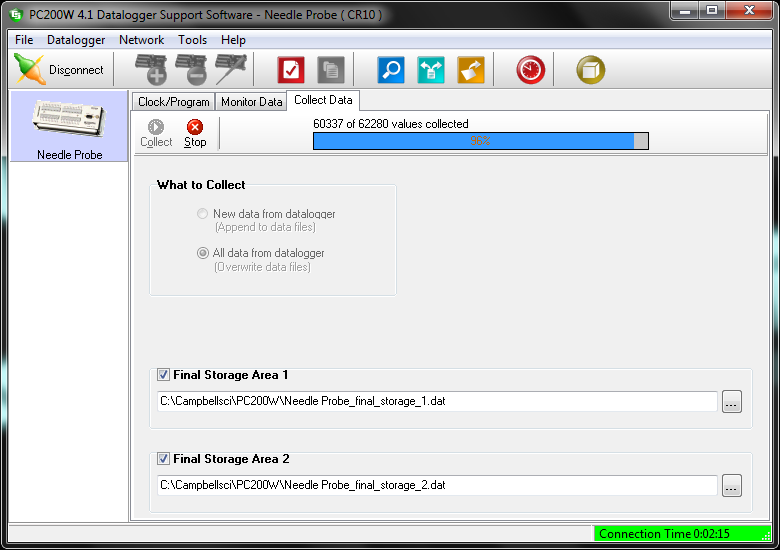
\includegraphics[width=0.8\textwidth]{fig/pc200w.png}
\caption{A screenshot of PC200W, the software used to pull data off the CR10X data logger.}
\label{fig:pc200w}
\end{figure}

Unlike the case of numerical experiments, it is extremely important in
real-world experiments---especially in the case of snow---to hand-inspect every
time/temperature curve. This is because, unlike the numerical experiments, there
is a significant chance that data will not be usable. In the case of snow in
particular, convection is typically experienced near the end of the heating
curve and the beginning of the cooling curve.

\begin{figure}[h]
\centering
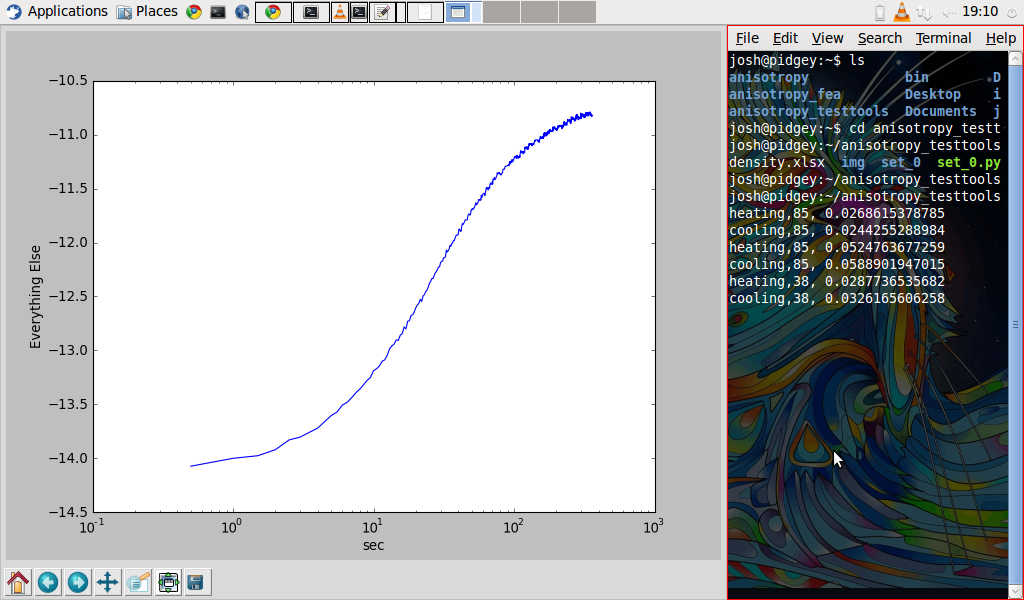
\includegraphics[width=0.8\textwidth]{fig/measurement_graph.png}
\caption{A plot of temperature vs. time from a real-world measurement of snow.
Each curve must be analyzed by-hand to check for such effects as convection, as seen on the right-hand side of this curve.}
\label{fig:meas_graph}
\end{figure}



\section{Snow Conductivity Measurements}

The first step in measuring proper snow is to make a vertical cut in the
snowpack, as in Figure \ref{fig:snowpack}.

\begin{figure}[h]
\centering
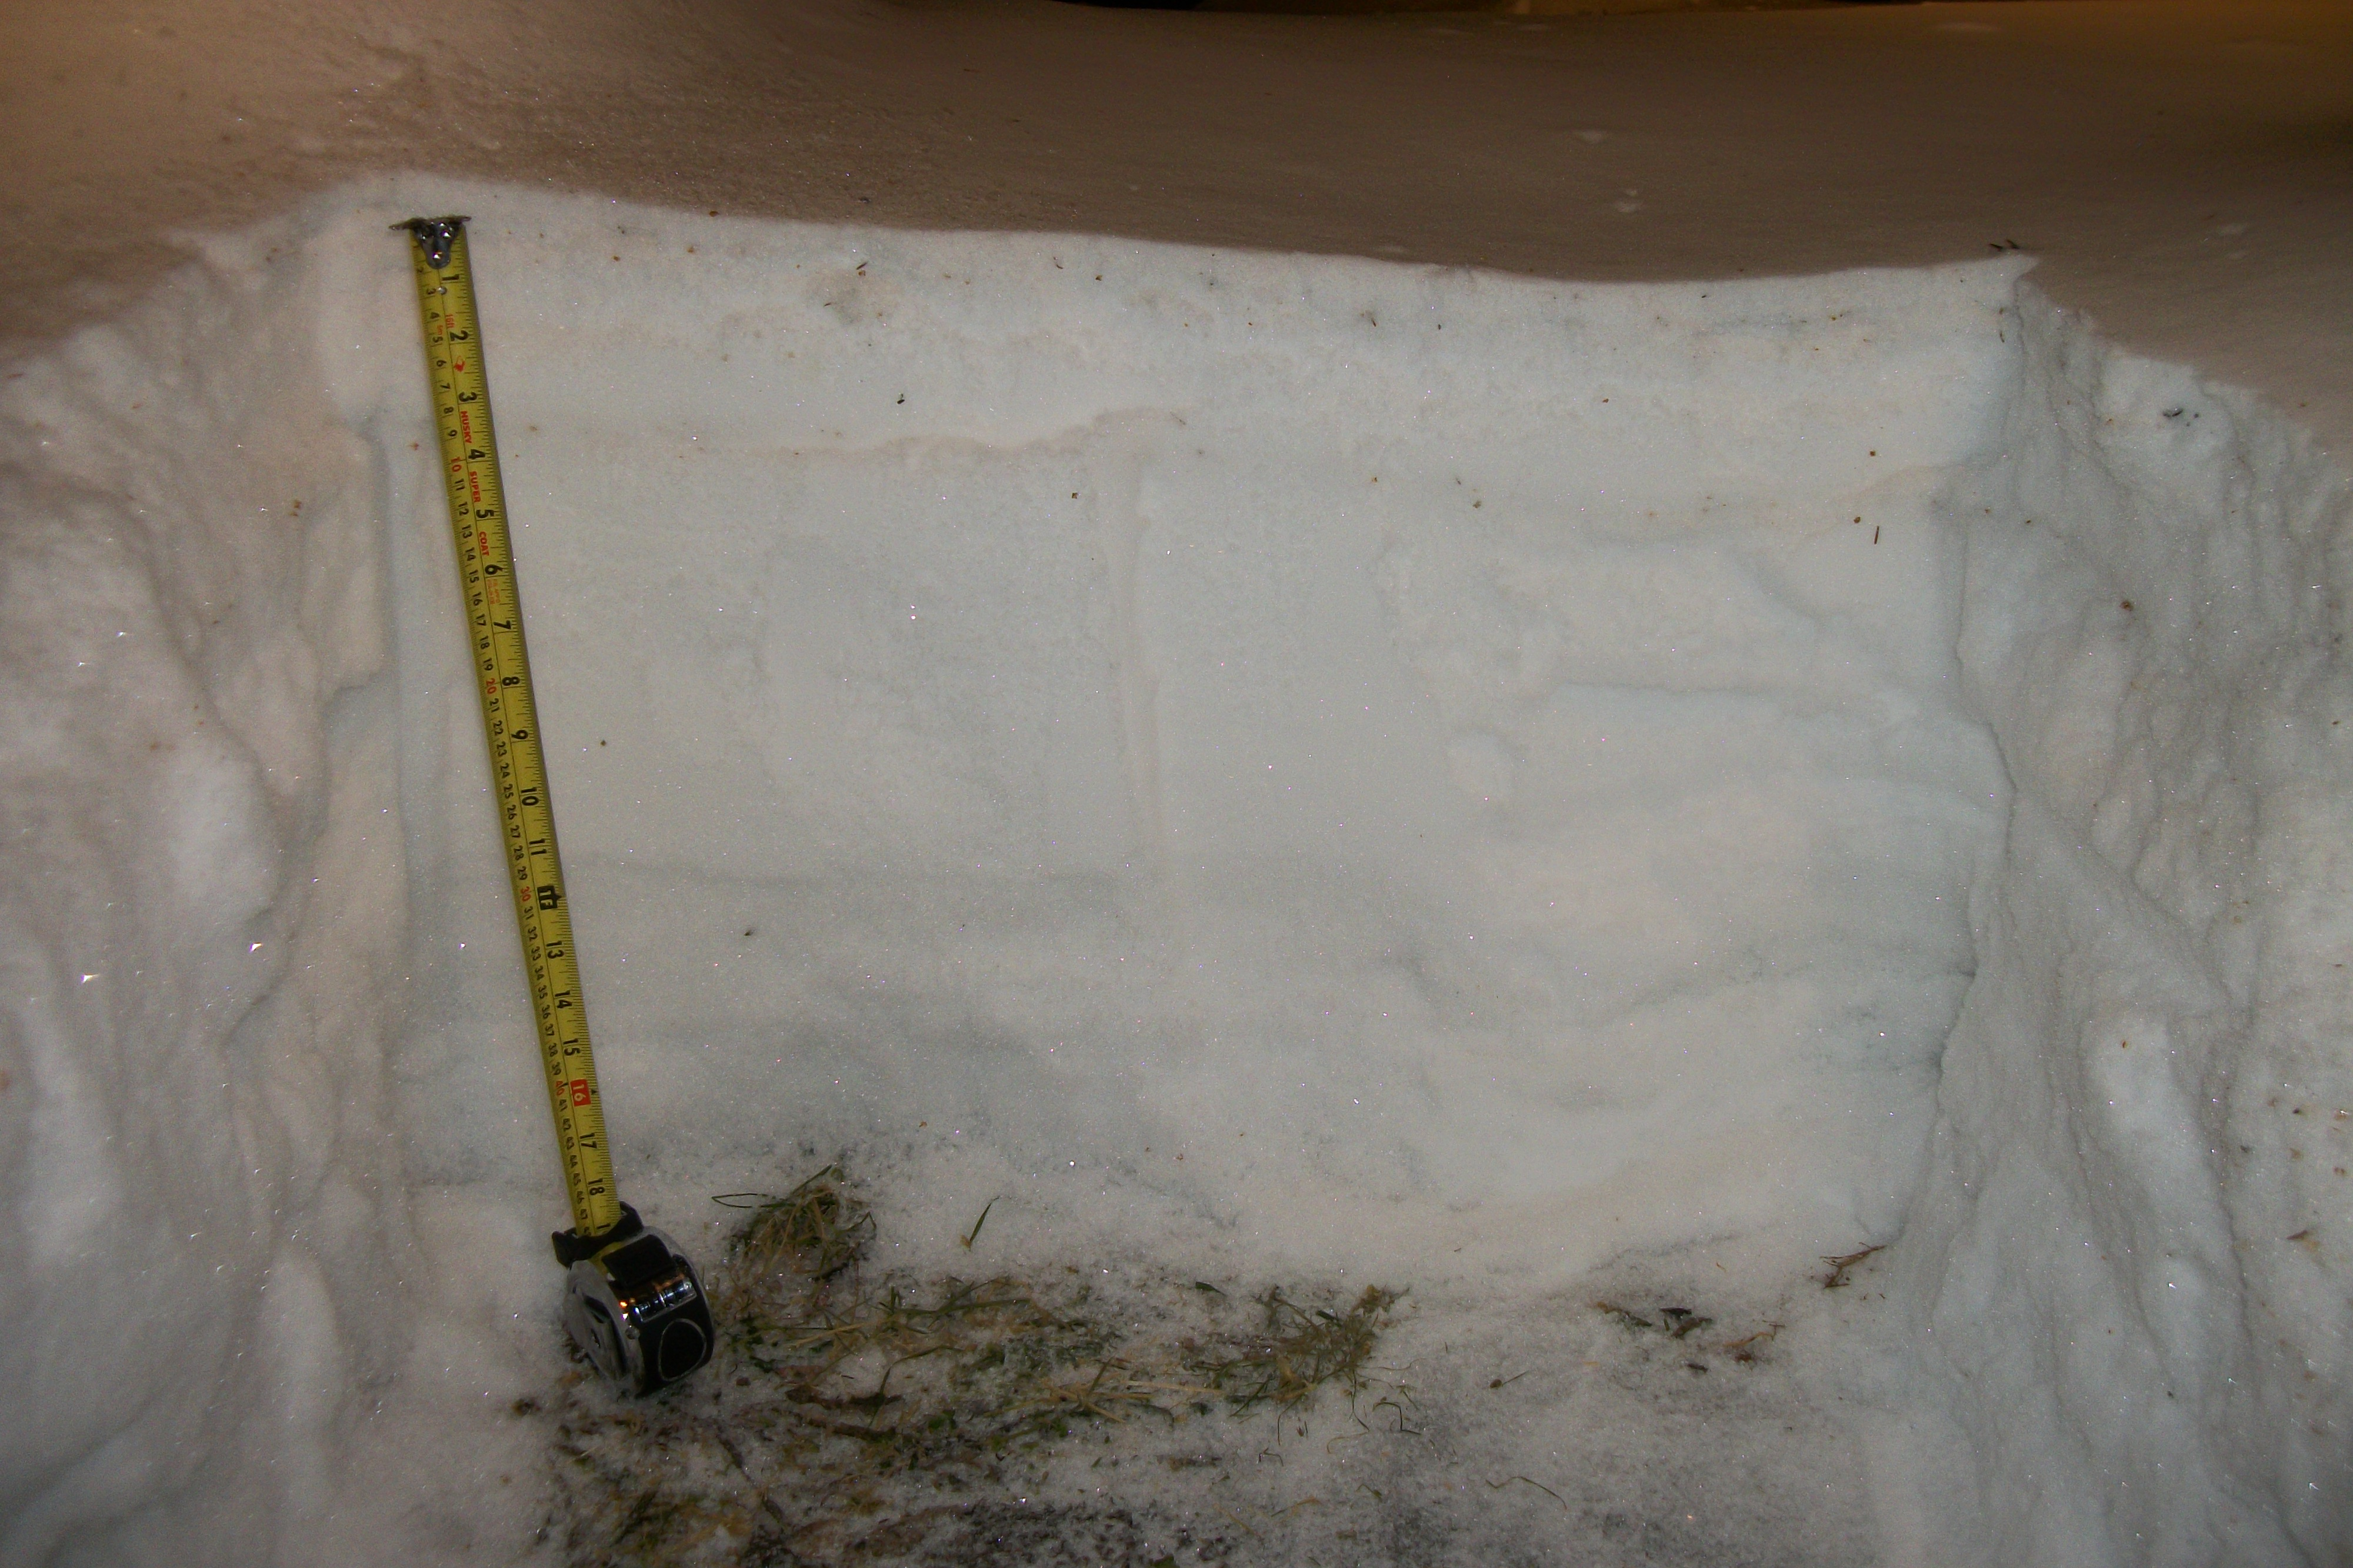
\includegraphics[width=0.8\textwidth]{fig/snowpack.jpg}
\caption{A close-up shot of tested snowpack.}
\label{fig:snowpack}
\end{figure}

Then, for every measurement, the needle is inserted into snow and a measurement
is taken. Snow is relatively difficult to work with due to the low structural 
integrity of the material.  The wire connecting the probe to the data logger is
stiff enough at low temperatures that situating the needle without ruining the
snowpack can be quite a challenge.

Along with each conductivity measurement, the height from the ground---measured
with a tape measure---and the angle of insertion---measured with a protractor
and a plumb bob---were recorded as metadata. In addition, for each series of measurements at a particular region, the density
of the snow is also measured with a cardboard cylinder (used as a control volume)
and a scale.

\begin{comment}
\begin{figure}[h]
\centering
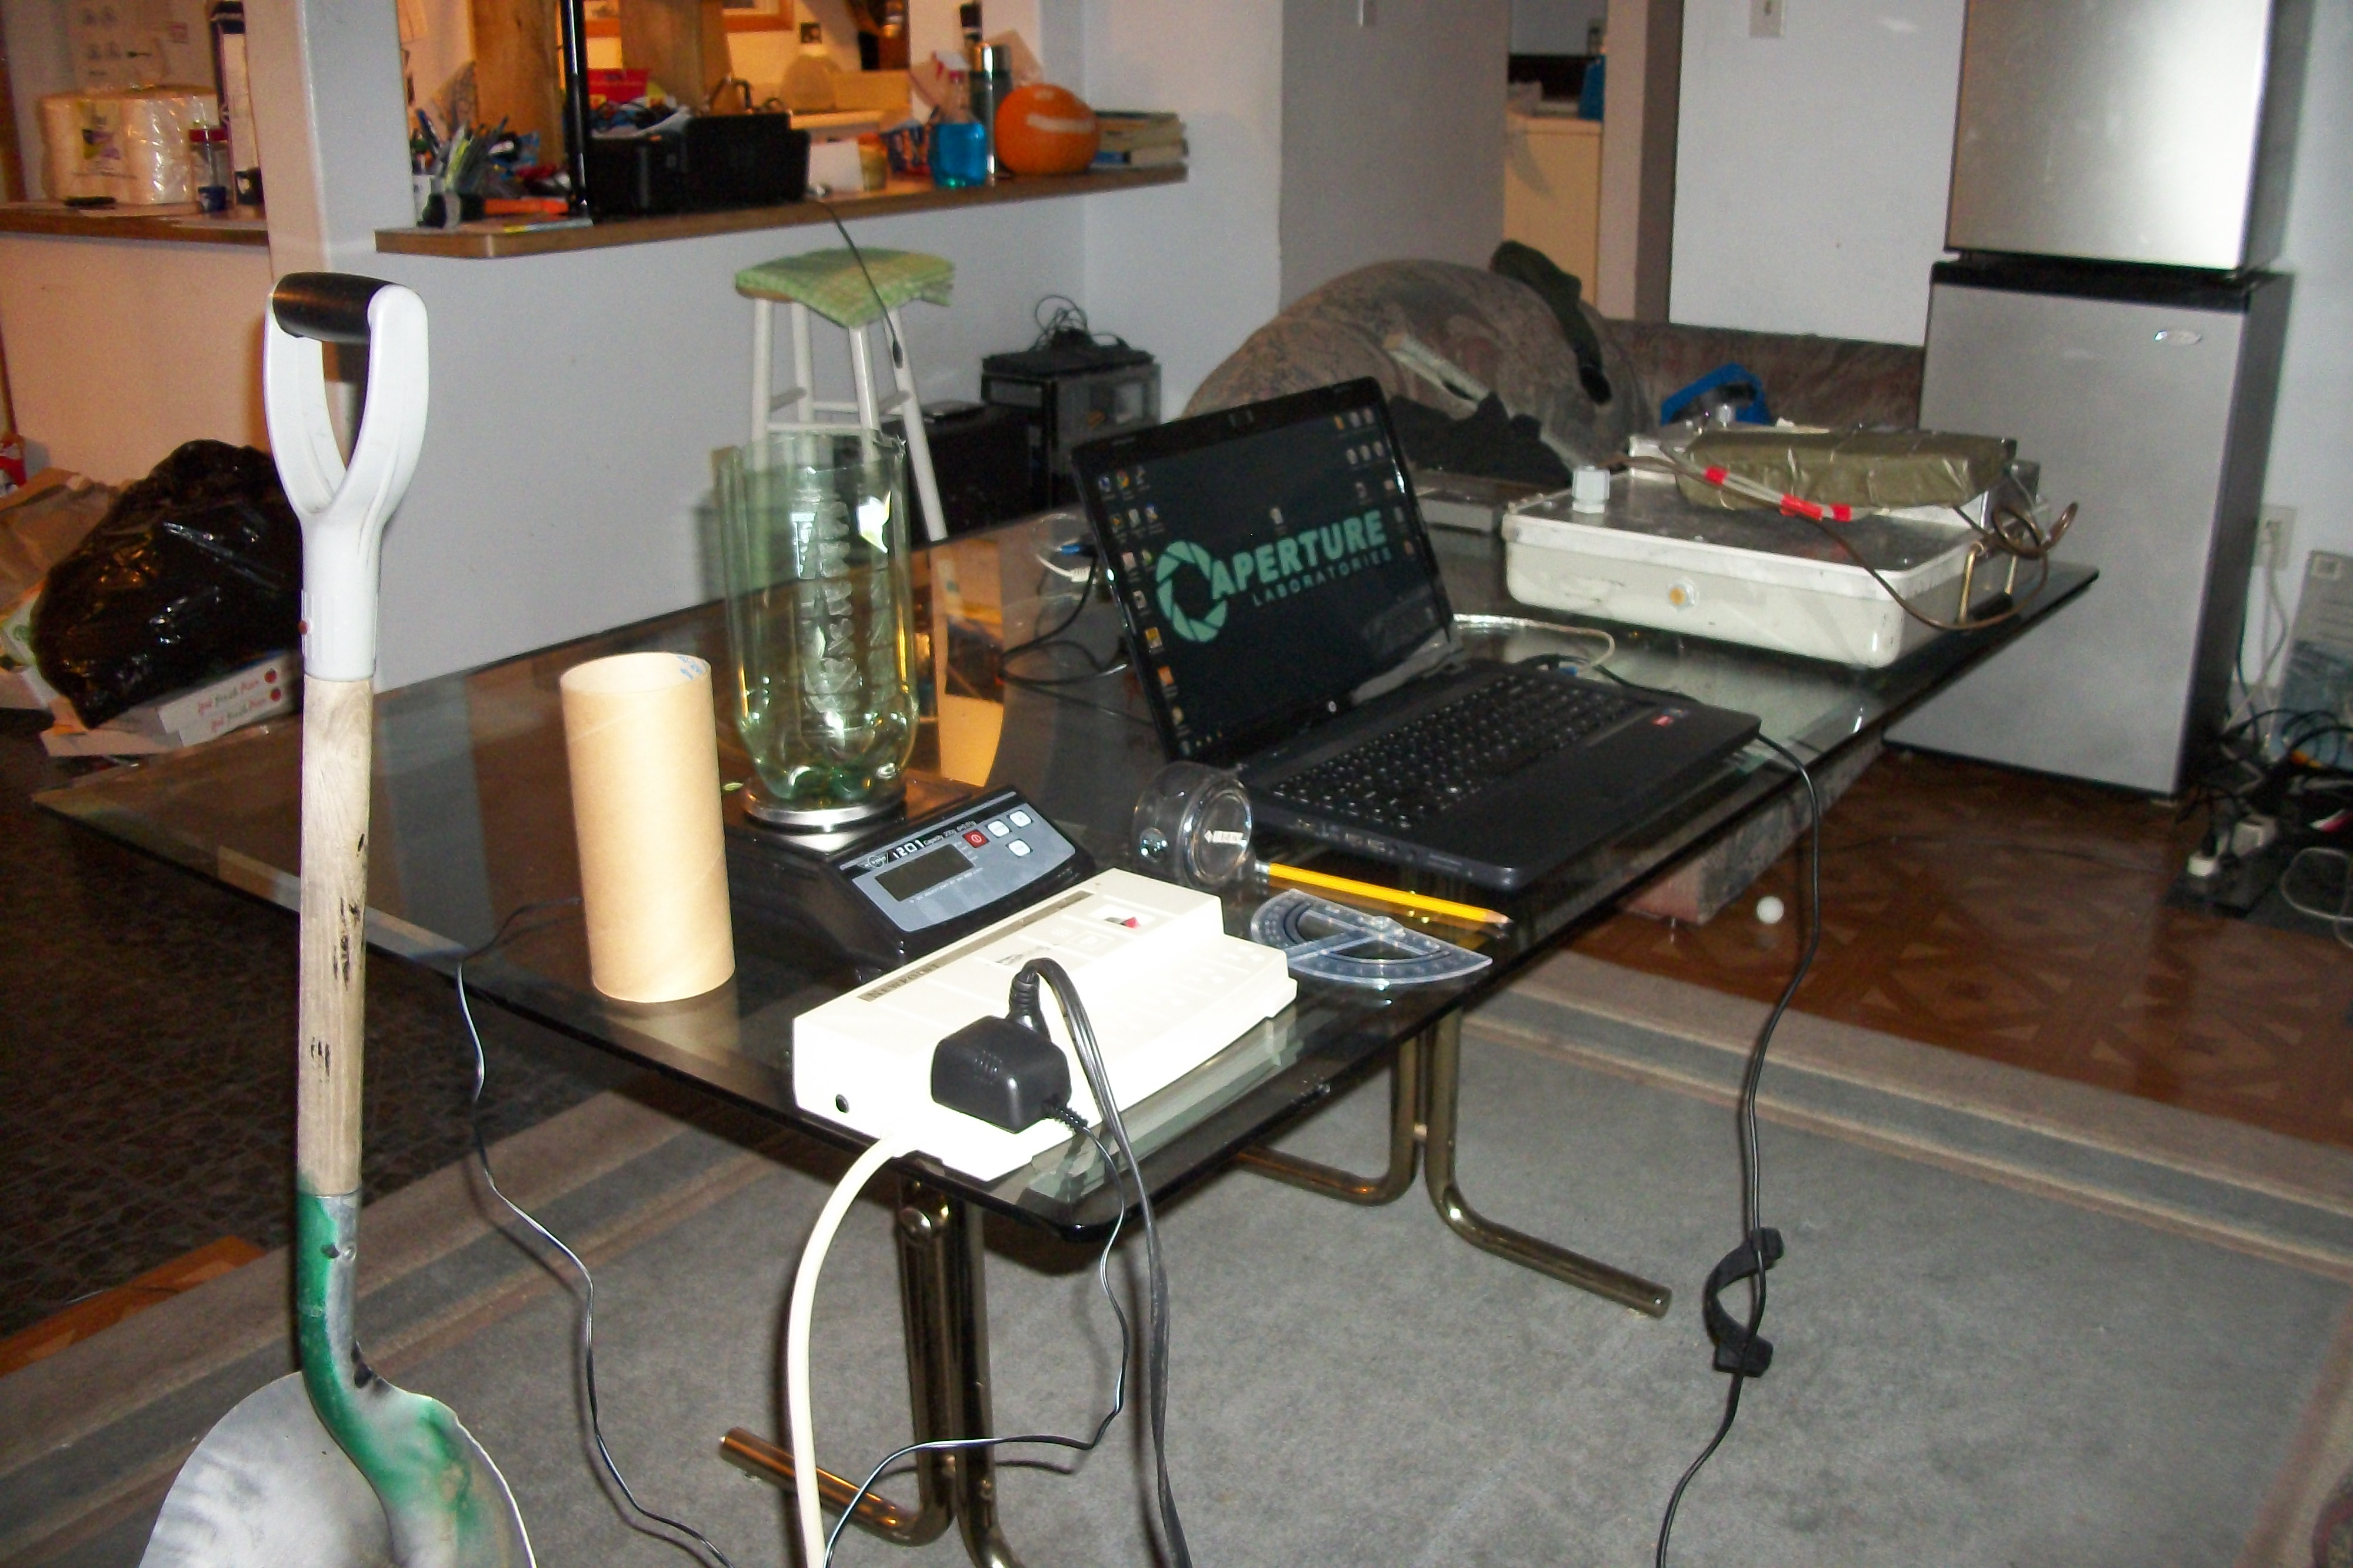
\includegraphics[width=0.8\textwidth]{fig/equipment.jpg}
\caption{Equipment used to measure snow thermal conductivity.}
\label{fig:equipment}
\end{figure}
\end{comment}

\begin{comment}
\begin{figure}[h]
\centering
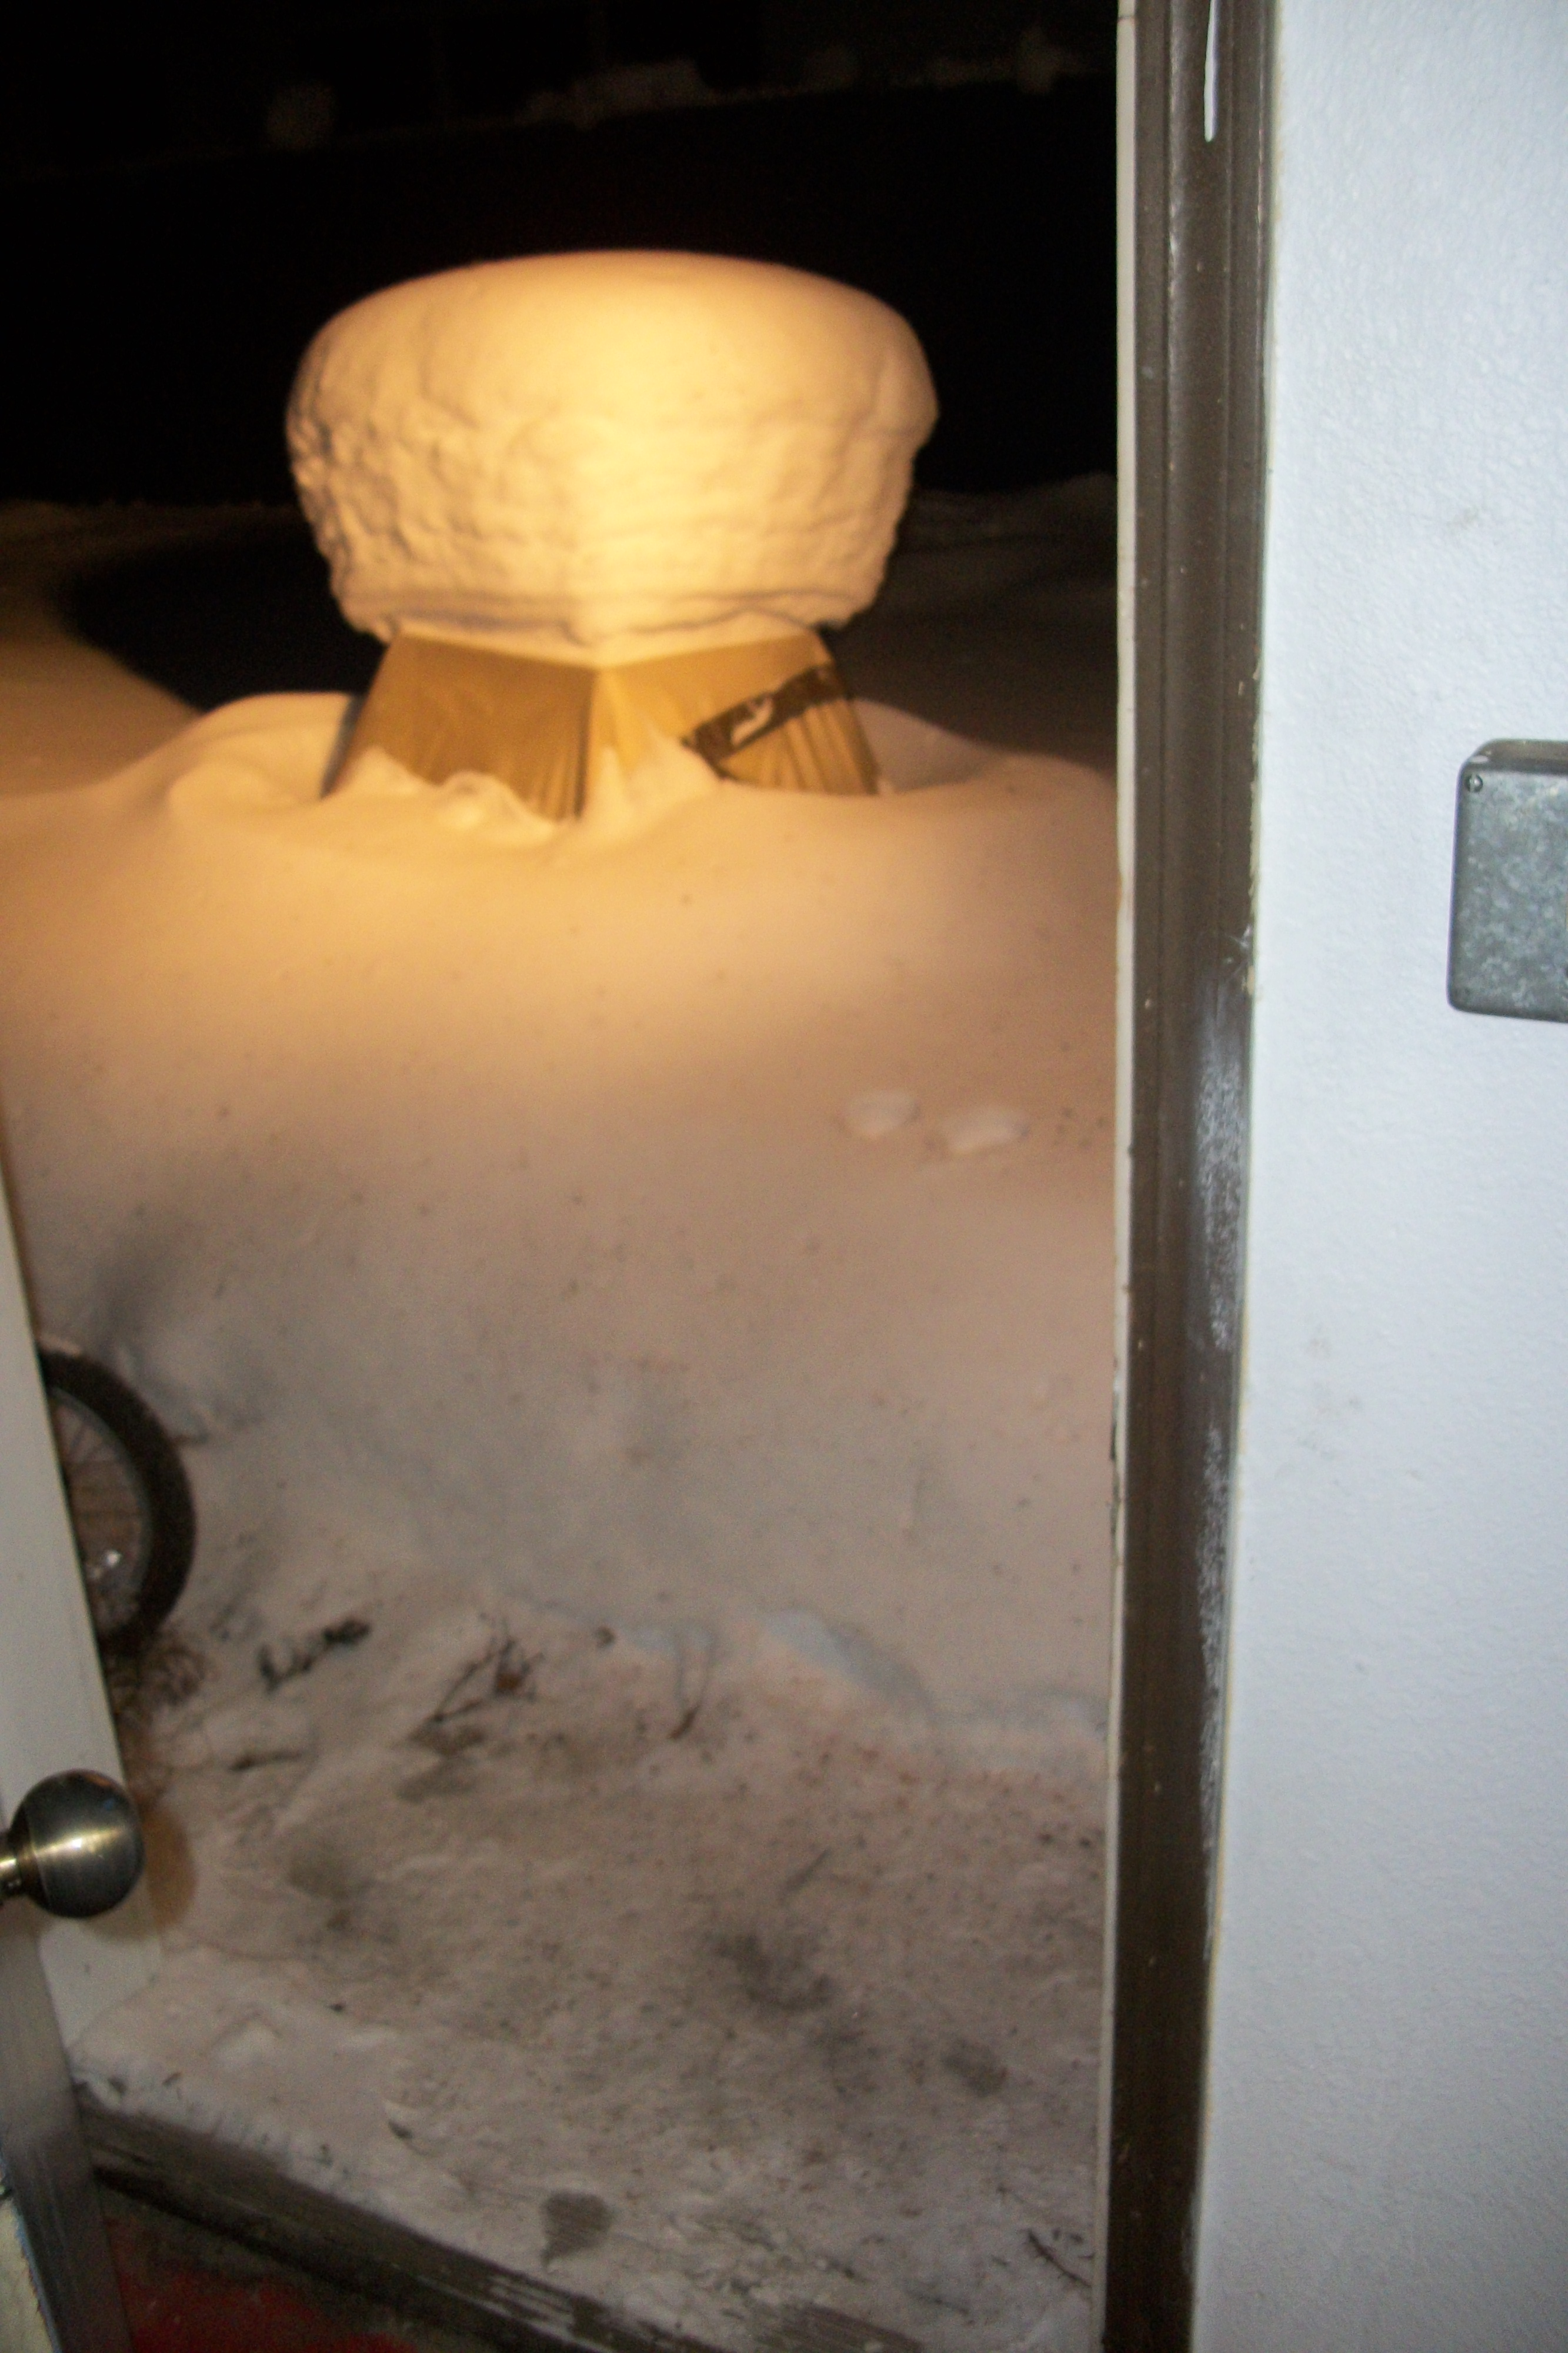
\includegraphics[width=0.4\textwidth]{fig/insitu_location.jpg}
\label{fig:insitu_location}
\caption{The location for in-situ tests.}
\end{figure}
\end{comment}

\section{Benchtop Tests}

A standard used to benchmark needle probes is to measure the conductivity of a
large Nalgene bottle full of glycerine and surrounded in insulating foam to
mitigate changes in room temperature. Glycerine was chosen because it
has almost the same conductivity as water and does not readily convect. Moreover,
glycerine does not leave an air gap between the needle and the surrounding
medium like many porous materials, such as snow, will.

A method for testing anisotropic measurements by using alternating
layers of more-conductive and less-conductive materials has been devised, based on
this glycerine benchmark test. However, instead of glycerine, the materials
used are table salt and table sugar.

\section{Raw Materials for the Anisotropic Composite}

Salt and sugar's conductivities alone were both measured using the needle probe
apparatus. These measurements resulted in conductivities of
\(0.225\) \(\textrm{W}/\textrm{m}/\textrm{K}\) and 
\(0.106\) \(\textrm{W}/\textrm{m}/\textrm{K}\), respectively.

\begin{table}[h]
\centering
\begin{tabular}{l l | l l | l l}
Material & \# & Heating & Cooling & Average & Standard Deviation\\
Pure salt & 1 & 0.222 & 0.220 & 0.225 & 0.015\\
 & 2 & 0.218 & 0.256 &  & \\
 & 3 & 0.216 & 0.219 &  & \\
Pure sugar & 1 & 0.108 & 0.113 & 0.106 & 0.008\\
 & 2 & 0.098 & 0.109 &  & \\
 & 3 & 0.094 & 0.113 &  & \\
\end{tabular}

\caption{Raw results of salt and sugar measurements after calculating conductivity. The multiple results were averaged for the purpose of predicting anisotropic conductivity of an alternately-layered medium.}
\label{tab:saltnsugar}
\end{table}

Assuming alternating layers of equal thickness, the anisotropic thermal
conductivities in the aggregate should be:

\begin{align}
k_{xy} &= \frac12 \left( k_{\textrm{salt}} + k_{\textrm{sugar}} \right) &= \boxed{0.166}\\
k_z &= 2 \left( \frac1{k_{\textrm{salt}}} + \frac1{k_{\textrm{sugar}}} \right)^{-1} &= \boxed{0.144}\\
\frac{k_z}{k_{xy}} &= \boxed{0.870}
\end{align}

Despite the conductivity of table salt being roughly twice that of sugar, the
anisotropic conductivity ratio is fairly close to one, meaning that the anisotropy
of the experimental medium, while significant, is relatively weak. Advantageously, however, salt and sugar are relatively inexpensive media to work with.

\section{Apparatus for Containing Anisotropic Composite}

\begin{figure}[h]
\centering
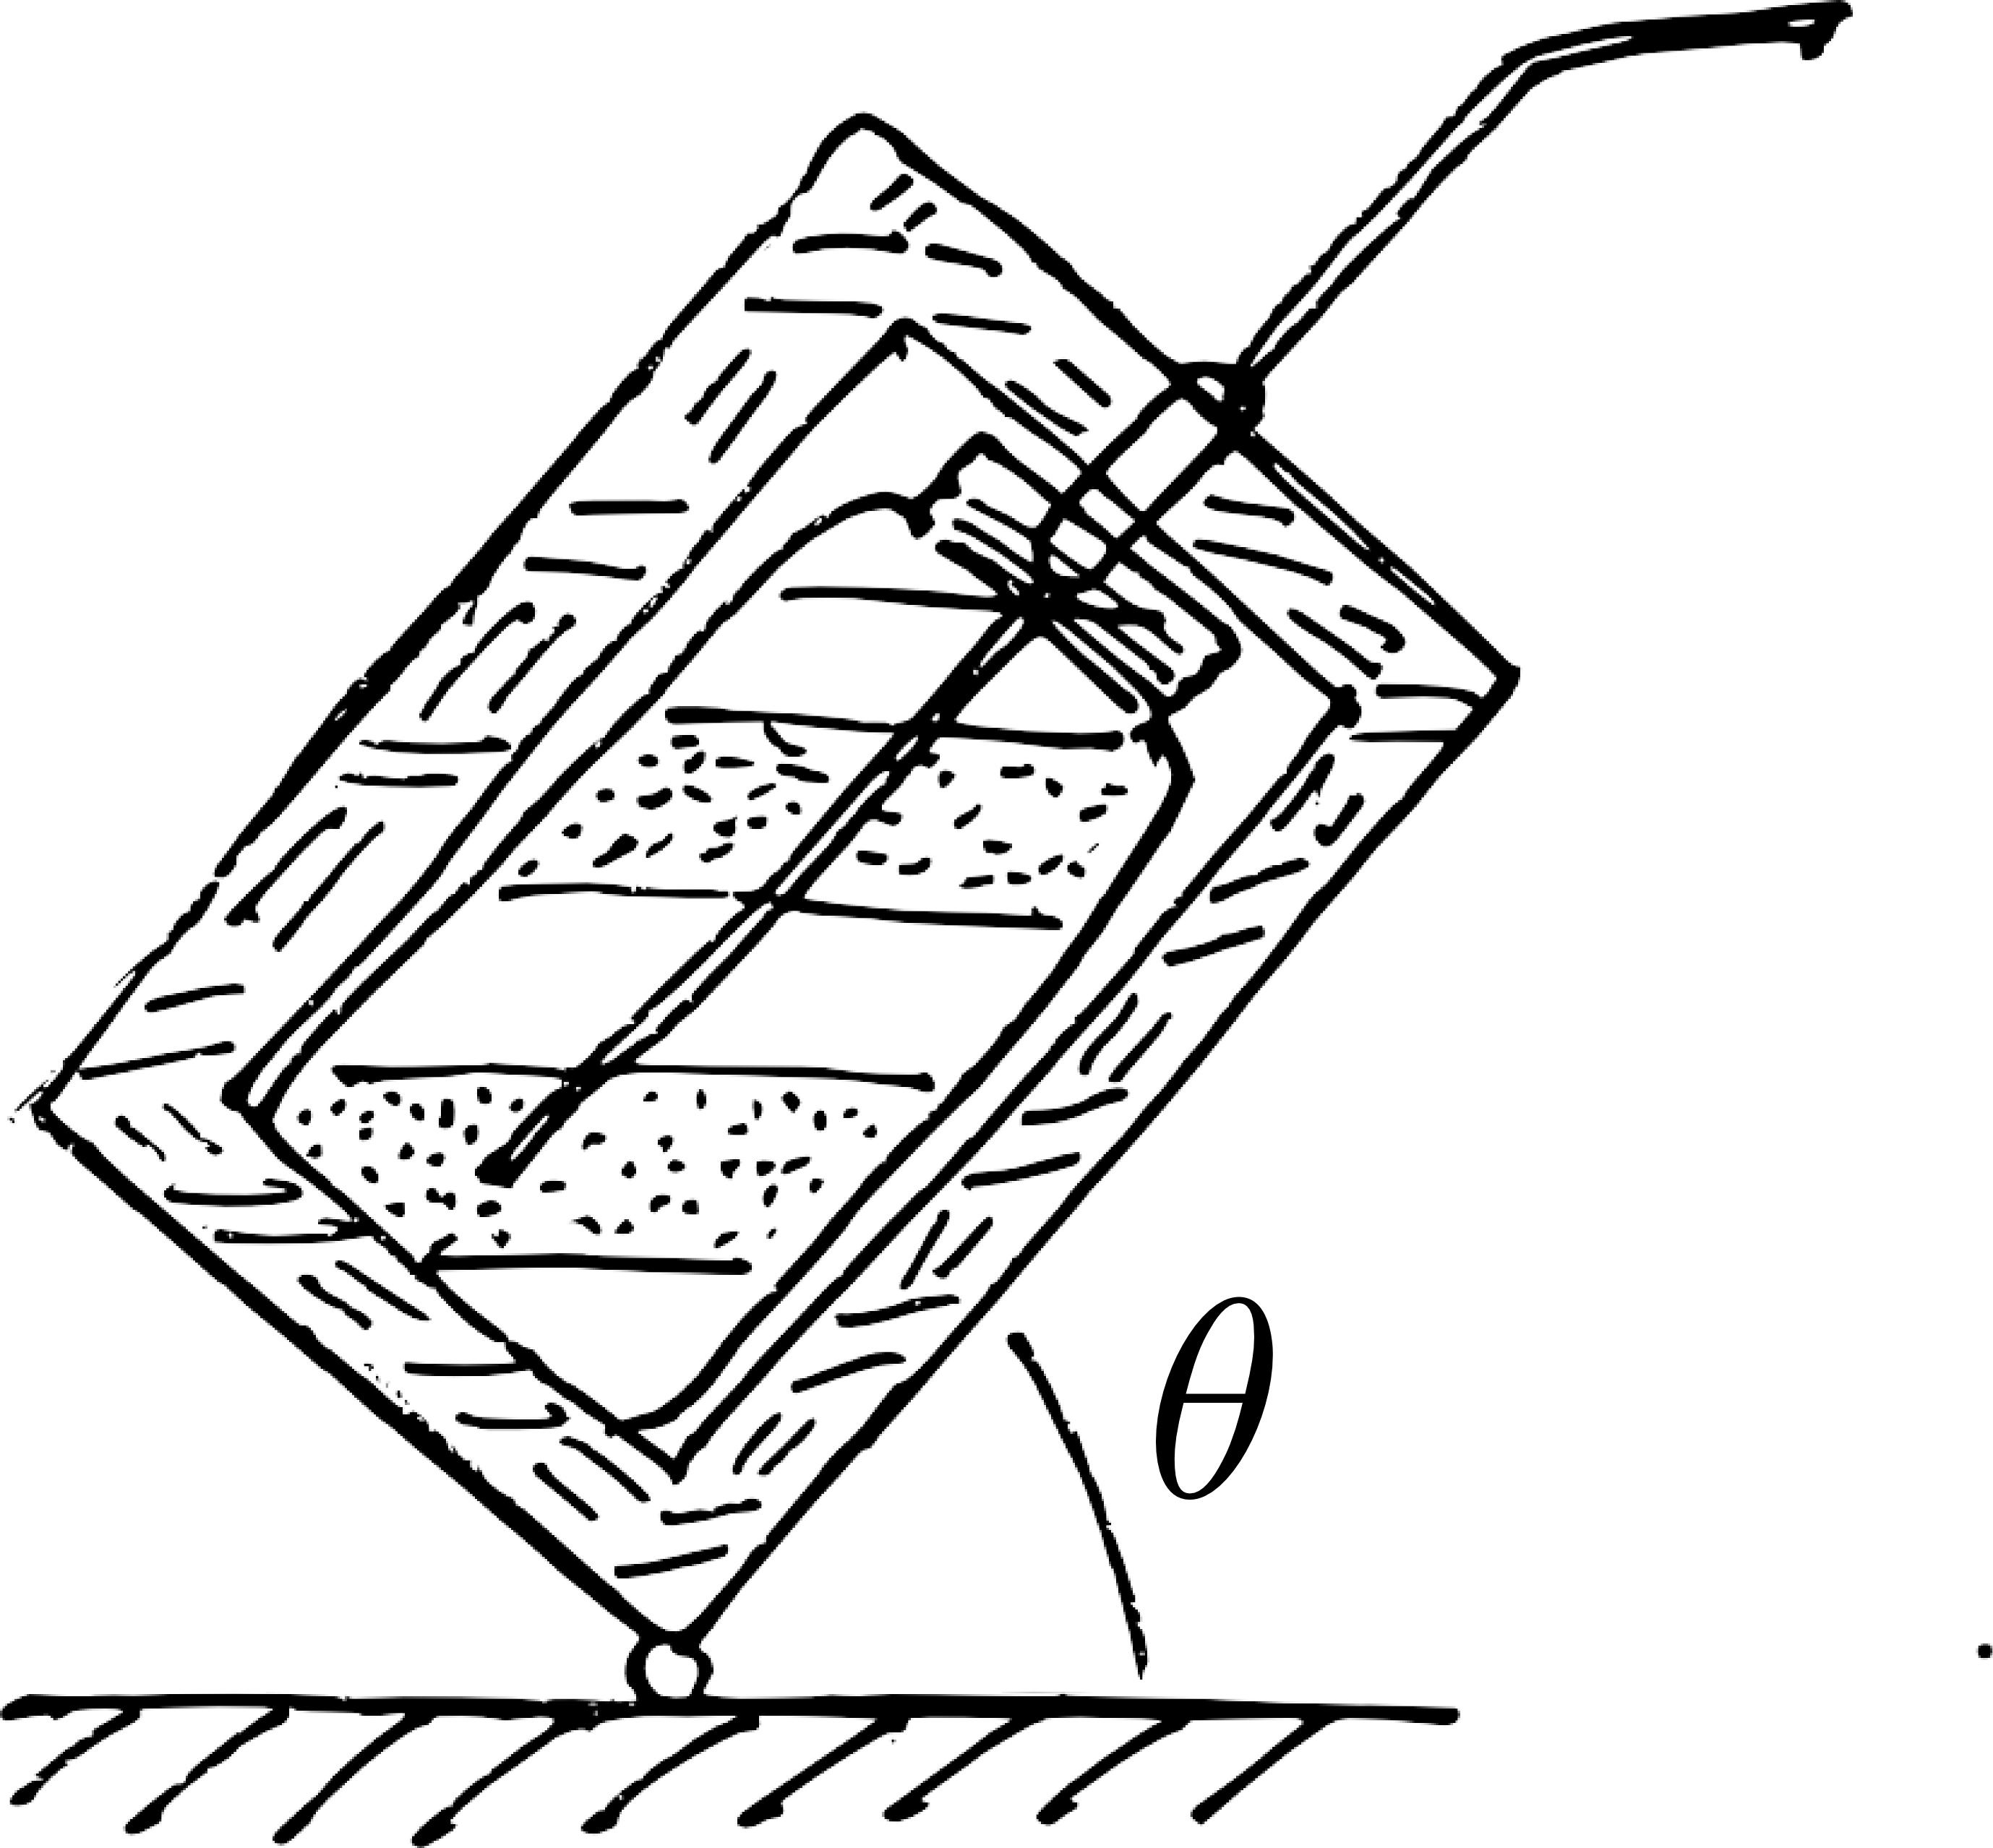
\includegraphics[width=0.4\textwidth]{fig/tilter_diagram.png}
\caption{An illustration of the apparatus used in benchtop measurements. The
apparatus was designed to tilt in order to cause alternating layers of self-
leveling materials to meet the needle at a given angle. However, the materials
actually used were not self-leveling, meaning the tilting apparatus was of 
limited utility.}
\label{fig:tilter_diagram}
\end{figure}

In order to effectively change the directions of anisotropy, a foam box for the
nalgene bottle was built that could be rotated on an axis and clamped in place.
The resulting angle from the horizontal can be measured with a protractor. The apparatus was designed with gels such as glycerine in mind, such that the layers
would self-level. However, because powders were used instead of gels, leveling
had to be done by hand, usually with a spoon. The sugar was dyed green in order
 to differentiate it from the salt.

\begin{figure}[h]
\centering
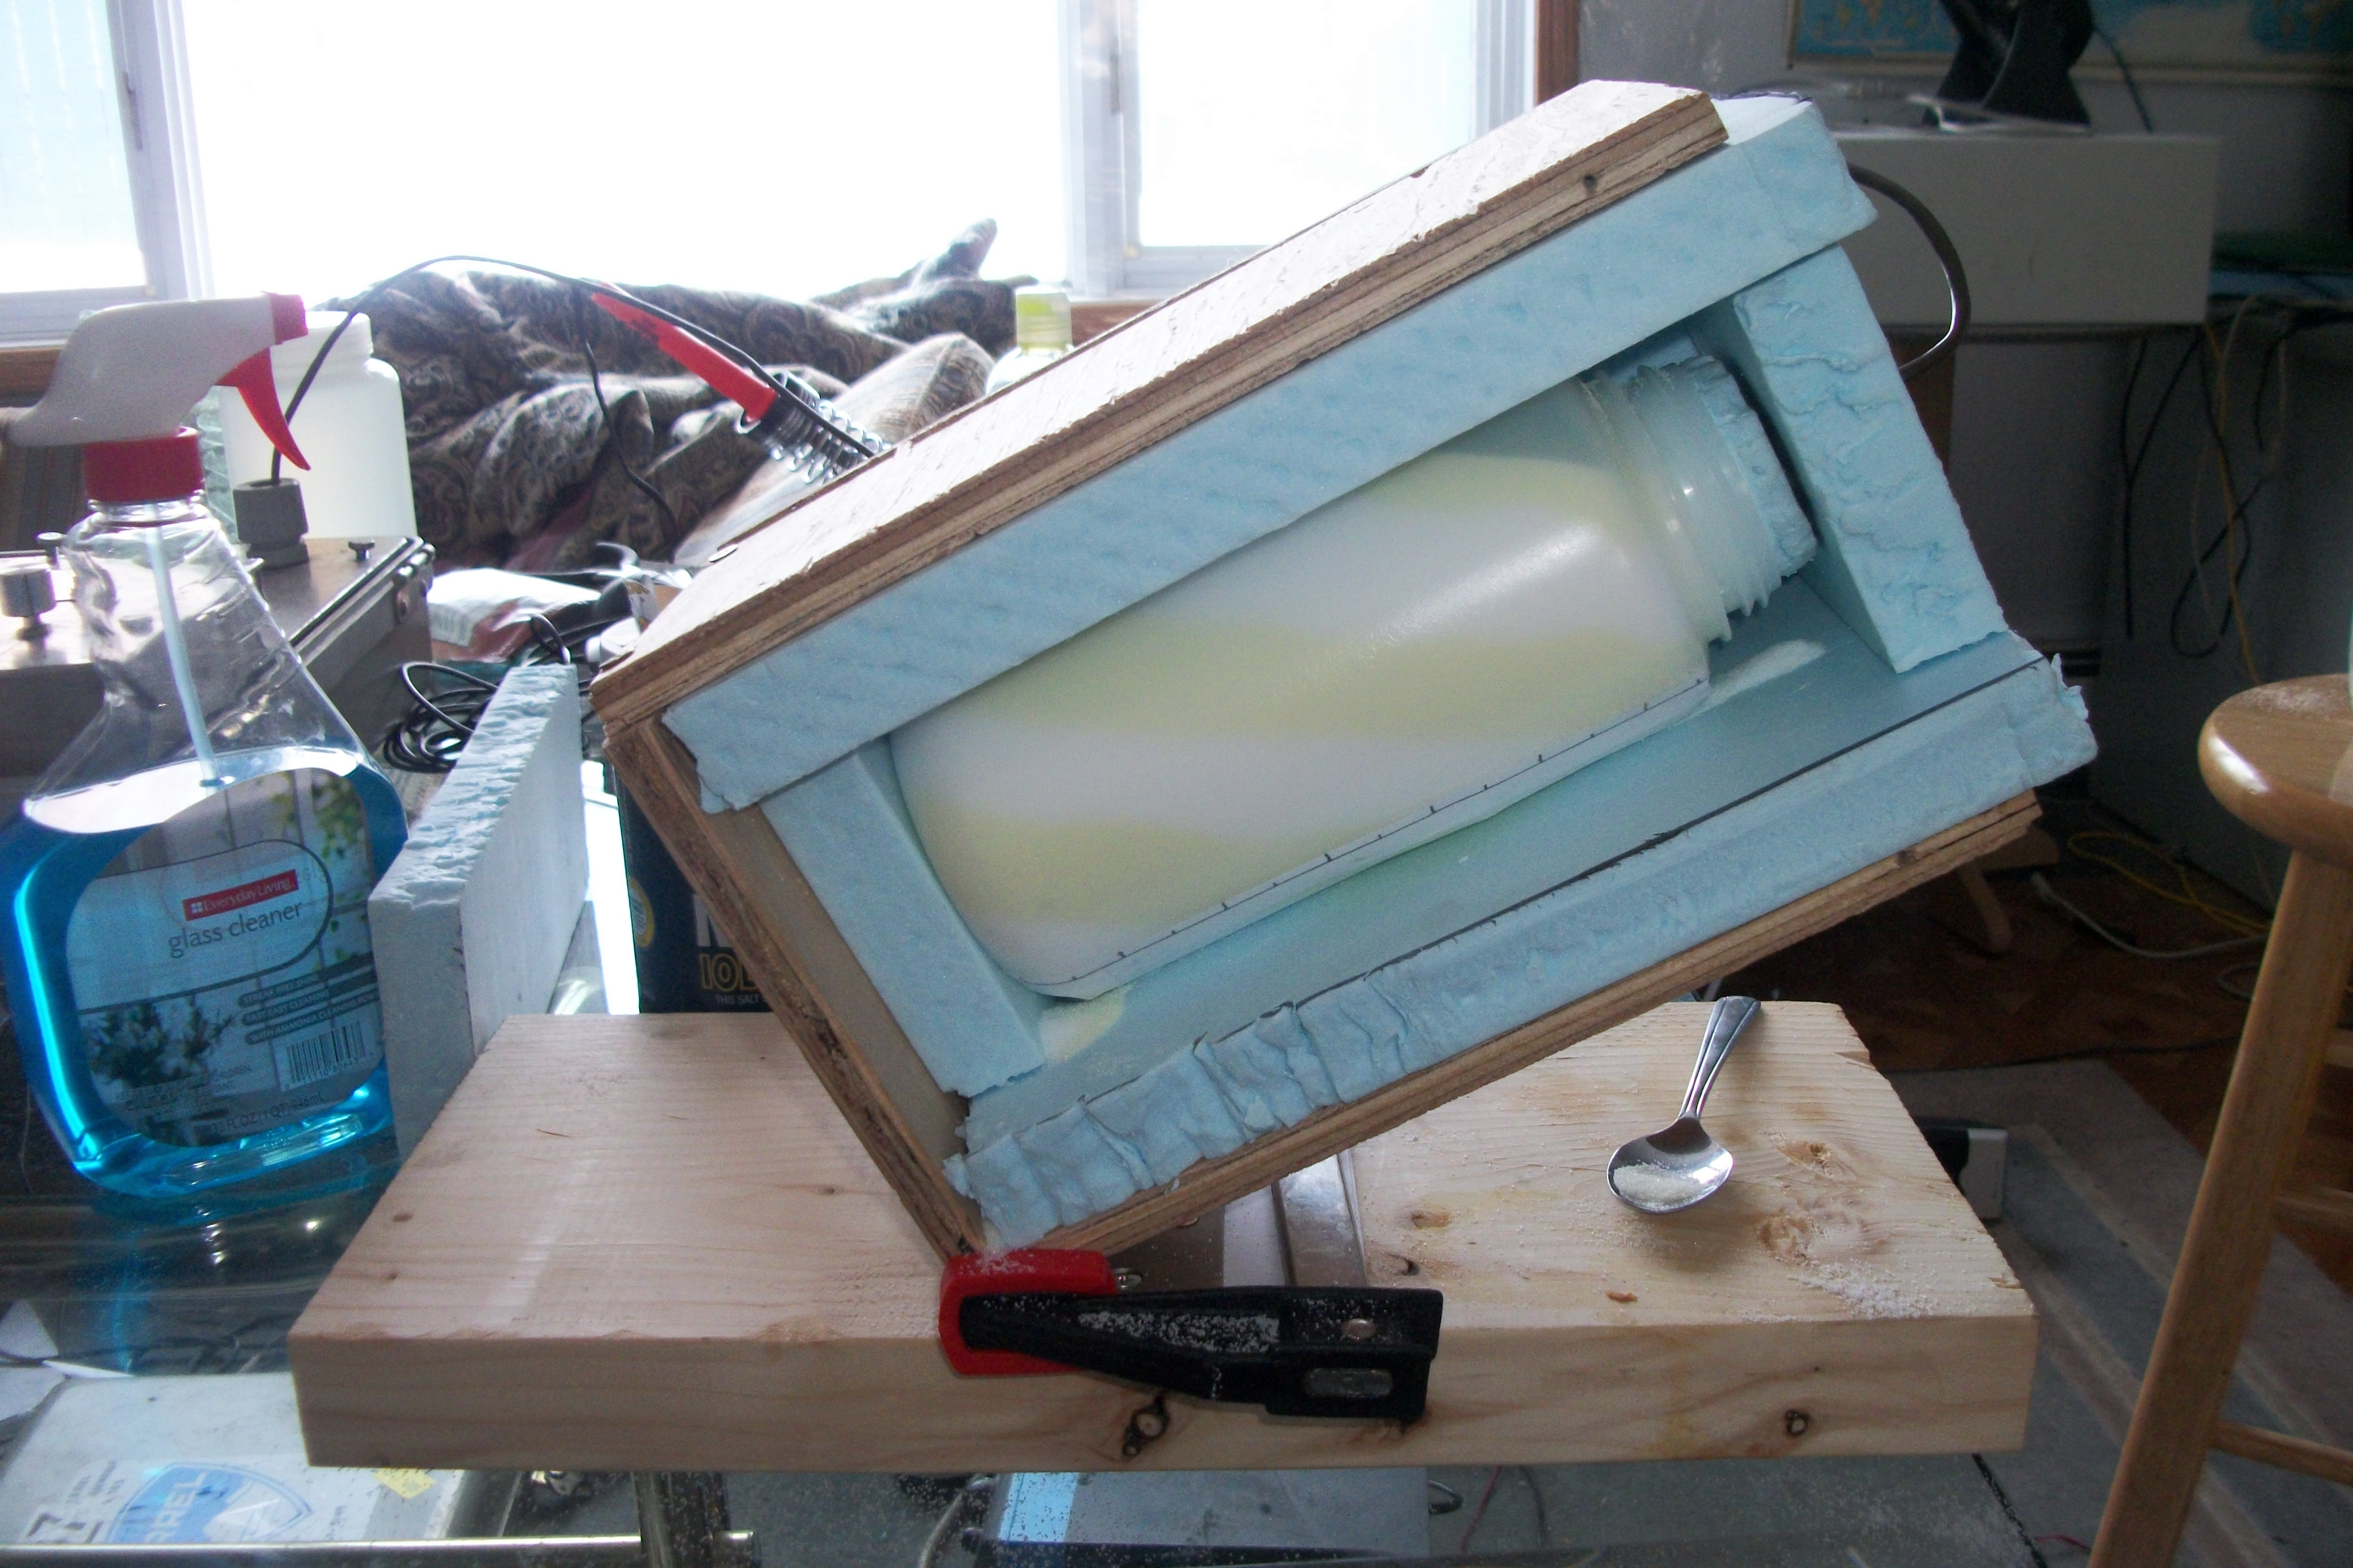
\includegraphics[width=0.8\textwidth]{fig/tilter_irl.jpg}
\caption{A photograph of the benchtop measurement apparatus in use, at 30 degrees.}
\label{fig:tilter}
\end{figure}

\chapter{Results and Interpretation}

\section{Parameters and Nondimensionalization}

For most analyses, many of the parameters and results are non-dimensionalized. In
particular, instead of separate parameters for \(k_z\) and \(k_{xy}\), \(k_z\)
and \(k_{\textrm{meas}}\) are both normalized by \(k_{xy}\). Numerical
experiments verified that this is permissible, as numerical experiments with
different \(k_z\) and \(k_{xy}\) parameters but equivalent ratios
\(\fracflat{k_z}{k_{xy}}\) resulted in very similar ratios of
\(\fracflat{k_{\textrm{meas}}}{k_{xy}}\).

Angle is an exception. In this analysis, all angles are given as degrees from
the horizontal (\(xy\)) plane.

\section{Numerical vs. Analytical Predictions}

A 3-D plot of the numerical and analytical predictions may be seen in 
Figures \ref{fig:numvanal}, \ref{fig:by_angle}, \ref{fig:by_kratio} and \ref{fig:angle0}.

\begin{figure}[h]
\centering
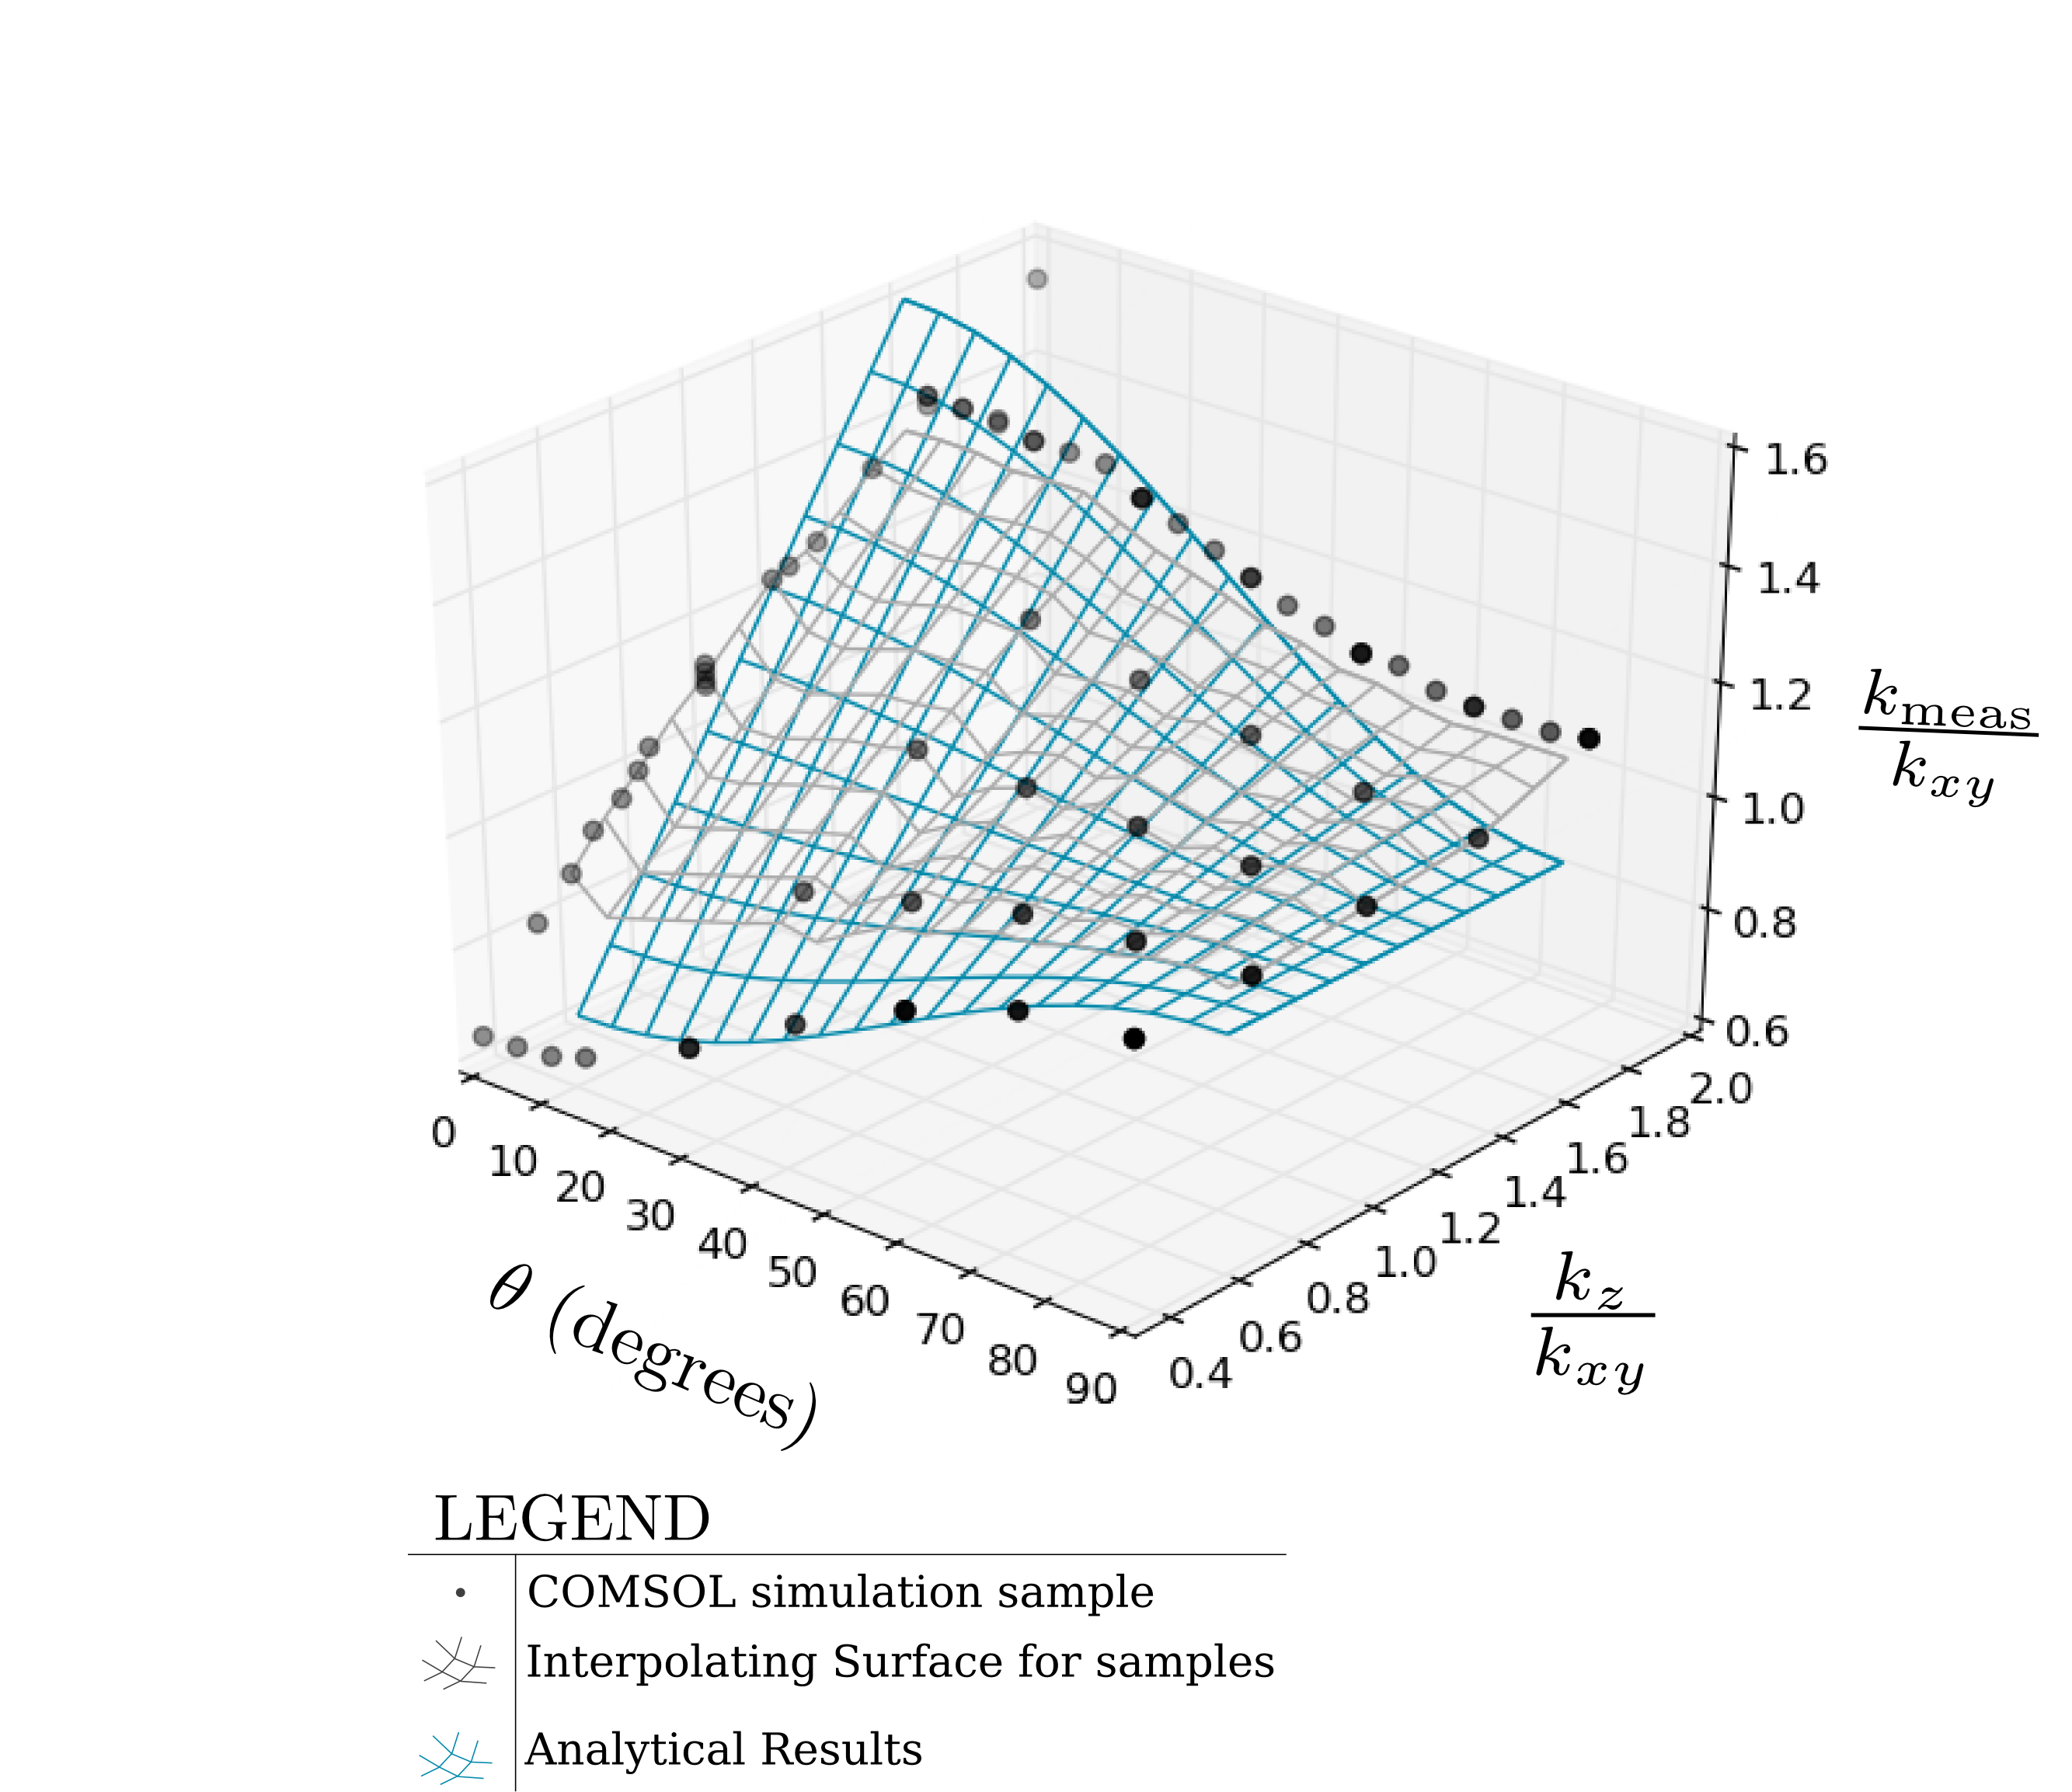
\includegraphics[width=\textwidth]{fig/numvanal.png}
\caption{A comparison of the numerical results and the analytical theory shows
general agreement. Grey dots represent numerical simulation results, the grey surface represents an interpolating surface of the dots, and the blue surface represents the analytical model. Disagreement between the two may be due to edge effects and/or numerical
model convergence issues.}
\label{fig:numvanal}
\end{figure}

\begin{figure}[h]
\centering
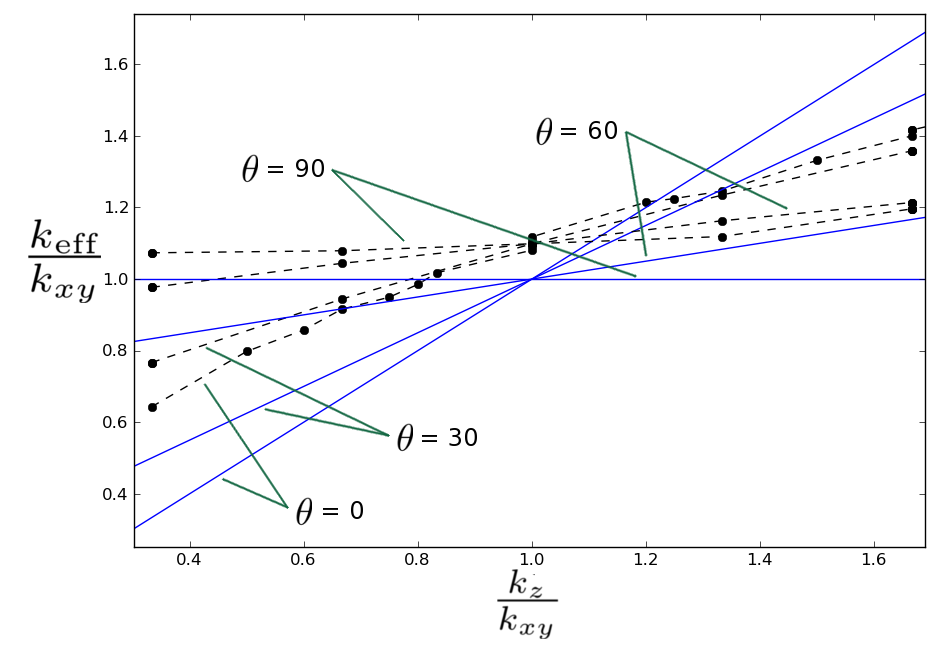
\includegraphics[width=0.6\textwidth]{fig/byAngle.png}
\caption{Slices of theoretical predictions by angle. Black represents numerical results, while blue represents analytical theory. It can be seen that the analytical theory predicts measured conductivity to be a stronger function of angle than the numerical data.}
\label{fig:by_angle}
\end{figure}


\begin{figure}[h]
\centering
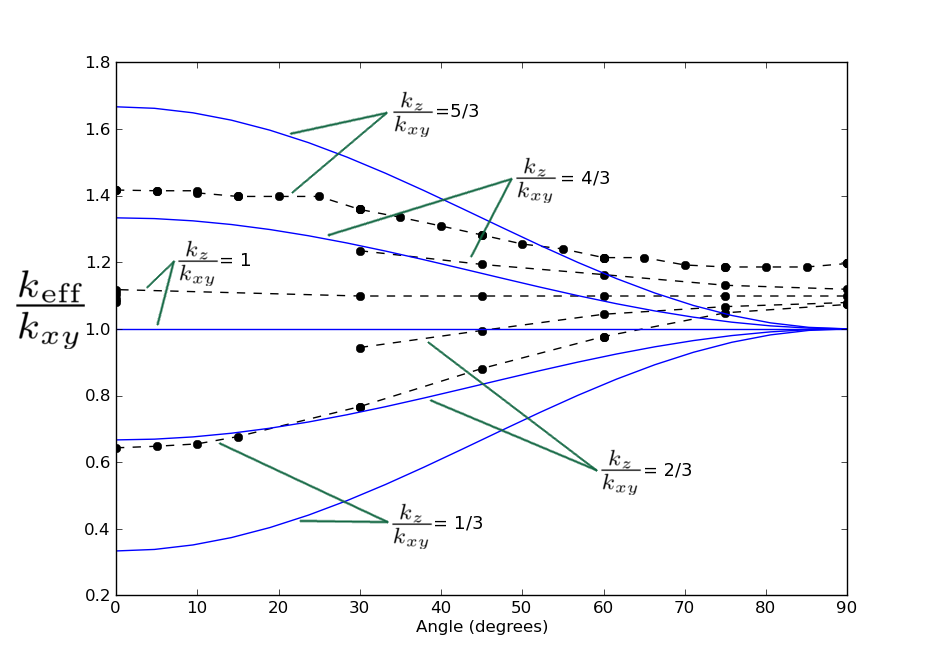
\includegraphics[width=0.6\textwidth]{fig/byKratio.png}
\caption{Slices of theoretical predictions by \(\flatfrac{k_z}{k_{xy}}\). Black represents numerical results, while blue represents analytical theory. It can be seen that the analytical theory
is perfect for the isotropic case (\(\flatfrac{k_{\textrm{meas}}}{k_{xy}}\), while the numerical experiments report larger-than-expected values.}
\label{fig:by_kratio}
\end{figure}

\begin{figure}[h]
\centering
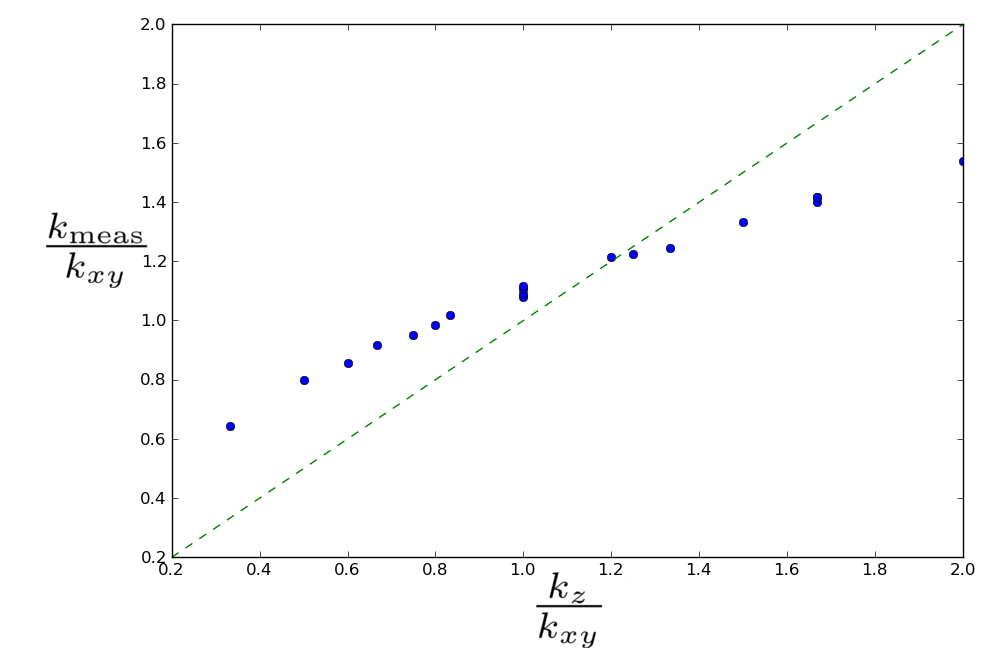
\includegraphics[width=0.6\textwidth]{fig/angle_0.png}
\caption{Theoretical predictions for the special case of \(\theta = 0\),
when the needle is oriented horizontally. Black represents numerical results, while green shows the line where \(k_{\textrm{meas}}} = k_z\), where measured conductivity and vertical conductivity are the same. The analytical predictions are indistinguishable from this line, and are therefore not plotted.
\label{fig:angle0}
\end{figure}


This plot shows that the two approaches to predicting measured conductivity
as a function of angle and anisotropy ratio are in general agreement. However,
there are subtle disagreements which may be important. For example, the
numerical model predicts overreporting of the thermal conductivity for
isotropic materials by about \(10\%\), and generally predicts smoother
curves for strongly anisotropic materials than the analytical approach.

There are two potential explanations for this: The first has to do with edge
effects, while the second has to do with convergence properties of the numerical
model.

In the first case, the numerical model accounts for edge effects by
modeling a finite length needle. Meanwhile, the analytical model does not take
into account edge effects, as it models an infinitely long needle like the
original needle probe method. The author conjectures that this is the mechanism
primarily responsible for the smoothing of \(k_{\textrm{meas}}(\theta)\) at more extreme
cases of anisotropy. In fact, for the isotropic case, these edge effects have
been studied and quantified analytically by other researchers. \cite{axialerror}


In the second case, the numerical model operates with a moderately coarse grid.
The convergence study results show that, while the time/temperature curves look
largely the same (Figure \ref{fig:conv_curves}), that the minor differences are magnified when taking the
derivative with respect to \(\ln(t)\) such that the coarse grid reports a
thermal conductivity of about \(110\%\) of the finer grid (Table \ref{tab:conv_kvals}). The author
conjectures that such effects may explain why the numerical predictions
consistently over-predict thermal conductivity as compared to the analytical
predictions, particularly in the isotropic case.


\begin{figure}[h]
\centering
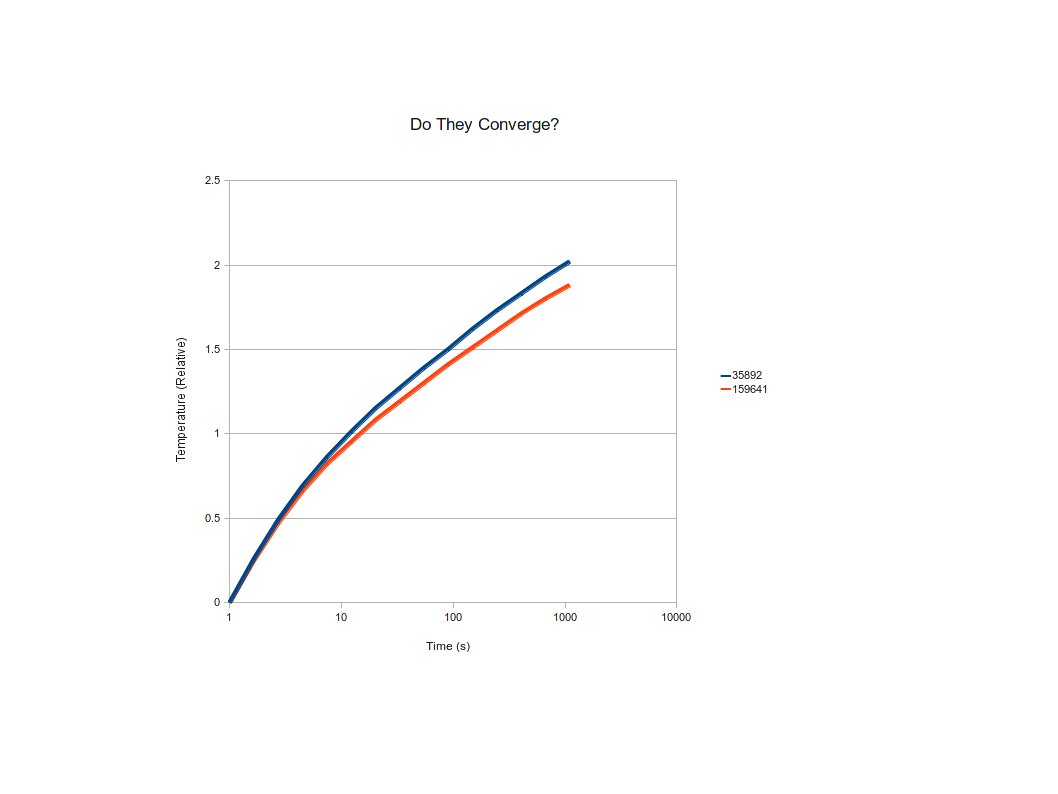
\includegraphics[width=0.6\textwidth]{fig/conv_curves.png}
\caption{A comparison of two \(T(t)\) curves from equivalent simulations with 
different fineness of mesh. These two curves appear quite similar, but their long-
time slopes are measurably different}
\label{fig:conv_curves}
\end{figure}


\begin{table}[h]
\centering
\begin{tabular}{r | l}
 & Slope\\
\(35892\) elements & 0.215\\
\(159641\) elements & 0.198\\
\% Error & 8.64 \%
\end{tabular}

\caption{A comparison of \(k_{\textrm{meas}}\) from two equivalent simulations 
with different fineness of mesh. Despite the similarities in time/temperature
curves, the resulting  conductivity calculations differ by nearly 10 \%. Units are in W\(/\)m\(\cdot\)K.}
\label{tab:conv_kvals}
\end{table}

\section{Benchtop Measurements}

The results of the benchtop measurements are mixed.

\begin{figure}[h]
\centering
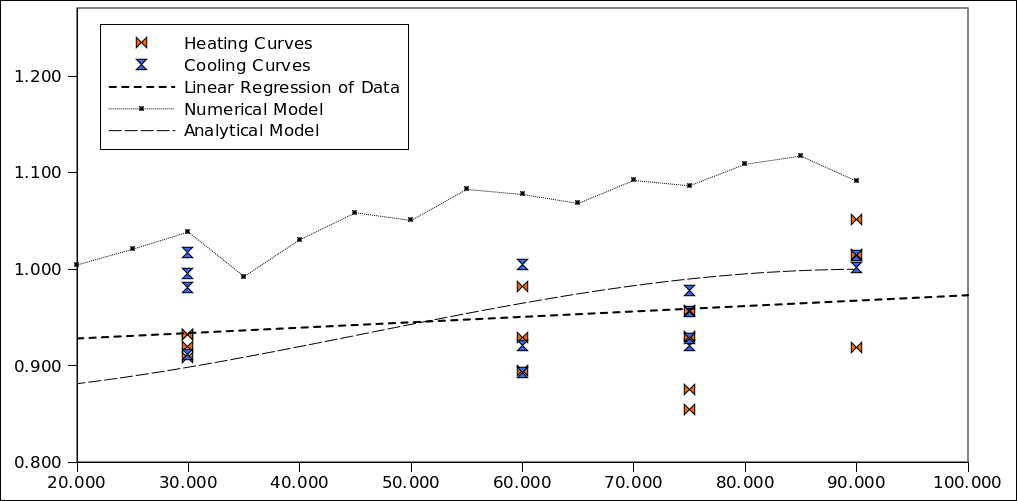
\includegraphics[width=0.9\textwidth]{fig/test_results.png}
\caption{A comparison of the benchtop measurements with the numerical and
analytical predictions, given the calculated anisotropic thermal conductivity.}
\label{fig:test_results}
\end{figure}

\begin{table}[h]
\centering
\begin{tabular}{l l | l l}
Angle (degrees) & # & Heating & Cooling\\
90 & 1 & 0.223284242942 & 0.243481576262\\
& 2 & 0.246684312618 & 0.24641641198\\
& 3 & 0.255505537961 & \sout{0.318256880271}\\
75 & 1 & 0.212791418373 & 0.223684883264\\
& 2 & 0.2325853424 & 0.232407779425\\
& 3 & 0.207604305022 & 0.225508200642\\
& 4 & 0.22608462065 & 0.237662896347\\
60 & 2 & 0.238543591267 & 0.244064408529\\
& 3 & 0.225850168518 & 0.22374914604\\
& 4 & 0.217518339596 & 0.216990054548\\
30 & 1 & 0.226573190917 & 0.238313150421\\
& 2 & 0.226429675463 & 0.247135960358\\
& 3 & 0.220619372302 & 0.241951060919\\
& 4 & 0.223387867071 & 0.221486604074\\
\end{tabular}

\caption{Raw data from the benchtop measurements. Note that one of the cooling curve measurements is striked out. This is because, when examined, it is clearly an outlier. Units are in W\(/\)m\(\cdot\)K.}
\label{tab:powders}
\end{table}


\begin{figure}[h]
\centering
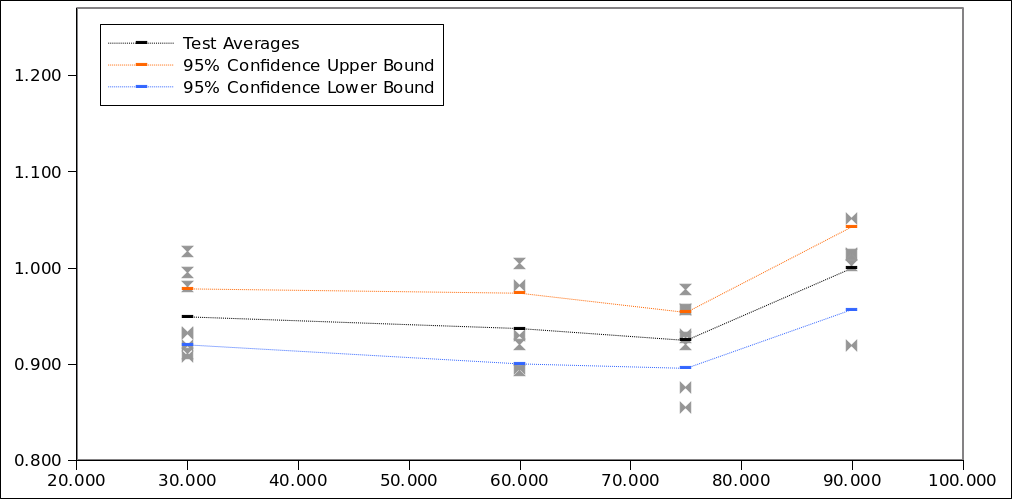
\includegraphics[width=0.9\textwidth]{fig/test_results_confidence.png}
\caption{Upper and lower bounds of 95 \% confidence in measurements. This analysis 
indicates that the measurements can not statistically exclude a null hypothesis.}
\label{fig:test_confidence}
\end{figure}

\begin{table}[h]
\centering
\begin{tabular}{r | l l l}
 & \multicolumn{3}{c}{ \(k_{\textrm{meas}} / \bar{k_{xy}}\) }\\
Angle & Mean & Standard Deviation & 95\% Confidence\\
90 & 1.000 & 0.0491 & 0.0431\\
75 & 0.923 & 0.0419 & 0.0291\\
60 & 0.937 & 0.0459 & 0.0367\\
30 & 0.949 & 0.0420 & 0.0291\\
\end{tabular}

\caption{Basic statistics on normalized benchtop measurements.  Units are in W\(/\)m\(\cdot\)K.}
\label{tab:pow-stats}
\end{table}


First, it may be seen that there is a significant amount of noise inherent in
the needle probe method, even accounting for obviously failed measurements.
This is likely due in part to the numerical derivative as well as the relatively
unpredictable behavior of porous materials. Given
this noise, it is difficult to see which of the two models is more appropriate.

Based on a general curve fit, the results show a slight upward slope, as
expected. However, given the variation in the results, it is statistically
possible that angle has absolutely no effect on the reading. This could be fixed
with more careful, exacting standards in the construction of the anisotropic
materials, more measurements at each angle, and measurements at more angles.
In other words, given the variance of the measurements, many more measurements
would have to be made in order to reach any statistically significant
conclusions, at least given the relatively amount of anisotropy of the sample.

Also given this noise and the relatively weak levels of anisotropy in the
sample, even with more measurements, it could still prove difficult to deduce
the degree of anisotropy of the sample with this data and a curve fit to either
the numerical or analytical predictions alone.

\section{In-Situ Snow Measurements}

% This would be a good thing for an appendix.
\begin{comment}
\begin{table}[h]
\centering
\begin{tabular}{l | l l}
\# & h (inches) & Angle (degrees)
5 & 10.5 & 85\\
6 & 10.5 & 85\\
7 & 13 & 38\\
8 & 12.5 & 45\\
9 & 10.5 & 92
\end{tabular}

\label{tab:metadata}
\caption{Height and angle measurements from snow measurements. The height data was unused in this analysis.}
\end{table}
\end{comment}

\begin{table}[h]
\centering
\begin{tabular}{r | l l}
Angle & Heating & Cooling\\
0 & 0.0289 & 0.0321\\
5 & 0.0269 & 0.0244\\
45 & 0.0290 & 0.0327\\
52 & 0.0288 & 0.0326\\
\end{tabular}

\caption{Conductivity results from the snow measurements. Units are in W\(/\)m\(\cdot\)K.}
\label{tab:snow}
\end{table}

\begin{table}[h]
\centering
\begin{tabular}{r | l}
Control Volume & \(736.76\) mL\\
Mass & \(161.14\) g\\
Density & \(0.219\) g/mL\\
& 219 kg/\(\textrm{m}^3\)\\
\end{tabular}

\caption{Measured and derived measurements for snow density. Units are in W\(/\)m\(\cdot\)K.}
\label{tab:density}
\end{table}

\begin{figure}[h]
\centering
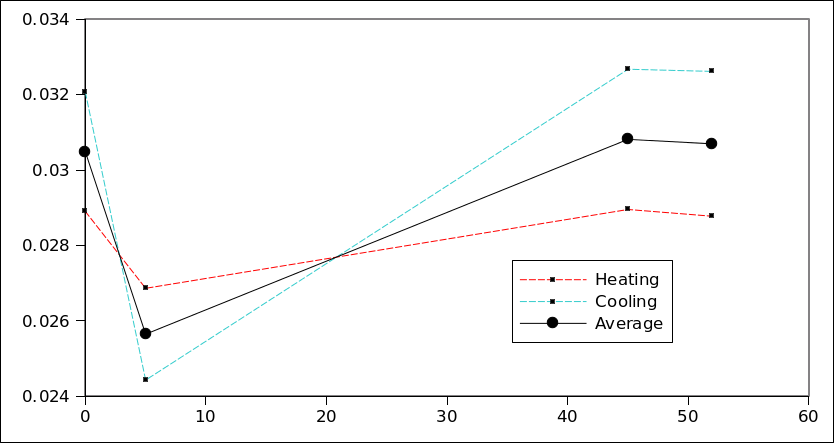
\includegraphics[width=0.9\textwidth]{fig/snow_meas.png}
\caption{Conductivity measurements in roughly the same layer of snow at various 
angles. Even a limited amount of in-situ snow measurements suggest a degree of
anisotropy.}
\label{fig:snow_results}
\end{figure}

\begin{figure}[h]
\centering
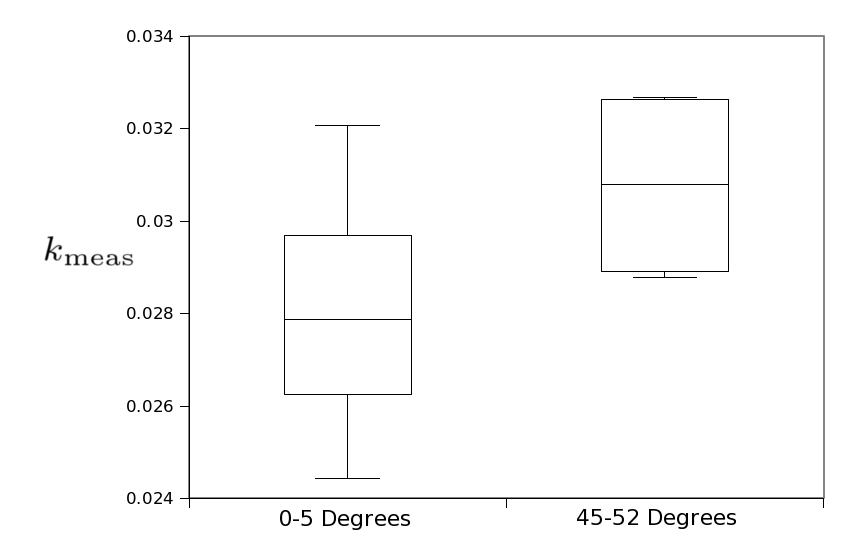
\includegraphics[width=0.9\textwidth]{fig/snow_meas_boxplot.png}
\caption{These boxplots give a general idea of the differences in measurements
between the near-horizontal angle and the more oblique ones in snow.}
\label{fig:test_boxplot}
\end{figure}


Due to the difficulty in taking snow measurements on top of the inherent noise
of the method, snow measurements are also inconclusive. However, the
measurements taken \emph{do} indicate anisotropy to a greater degree of confidence
than the benchtop measurements. Like the case of the benchtop measurements, with so few
measurements a curve fit against either method of prediction is unlikely to
yield useful results.

\chapter{Future Work}

\section{Introduction}

This is clearly not the end of research on this method. While the groundwork has
been laid, there are plenty of avenues which need more study.

\section{Assumptions in the Analytical Approach}

In the analytical model presented here, the needle is assumed to be of zero
thickness, and yet an average temperature over an ellipse is taken which
represents the needle surface.  The model seems to work relatively well; however, there are
other ways to represent such a problem that may yield more accurate results. For
example, one may be able to approach the problem in terms of a needle with a
finite thickness, in which case the solution to the problem should be an
infinite series of Bessel functions in the isotropic case. One may be able to
tackle the problem from a finite-thickness needle approach for better results. In addition, a refined model could account for edge effects. \cite{axialerror}

Another recommendation for future study is to build a hybrid method, which uses
the projection technique developed for the analytical method to specify a 2D
problem, but uses a finite element method to solve the 2D problem. Since this
new finite element model would not account for edge effects, it could be used to
help the causes of the discrepancies between the models. Moreover, since 2D
problems are much easier to solve, experiments may be ran at very high mesh
resolutions as compared to the 3D problem.

\section{Extended Convergence Study}

While a convergence study for the numerical model was undertaken, it was relatively
informal, and executed for only one particular configuration of parameters. A
more thorough investigation of the convergence properties of the numerical model
should likely be undertaken, especially in light of the \(10\%\) error observed
in the convergence study done in this work.

\section{Improved Benchtop Method}

The benchtop apparatus was based on the use of glycerine and agar gels for
calibration. However, the current anisotropic benchtop method uses sugar and
salt. This makes the proper layering of the materials difficult. Moreover, the
device is limited to a tilt factor of \(30\) degrees from horizontal due to the
location of the bottle's opening. Presumably, this method could be improved upon
to allow for more accurate material layering and for an increased range of
needle angles.

In addition, the materials used only lend themselves to an anisotropy ratio of
87\%. There is plenty of room for improvement, in terms of suitable materials.
Figure \ref{fig:anisovmatl_rats} shows what material conductivity ratios are
required to achieve a given anisotropic conductivity ratio, assuming
equal-thickness layers. While salt and
sugar fare poorly, real-world materials have a wide range of conductivities
such that two materials with sufficiently different conductivities should be
possible to find.

\begin{figure}[h]
\centering
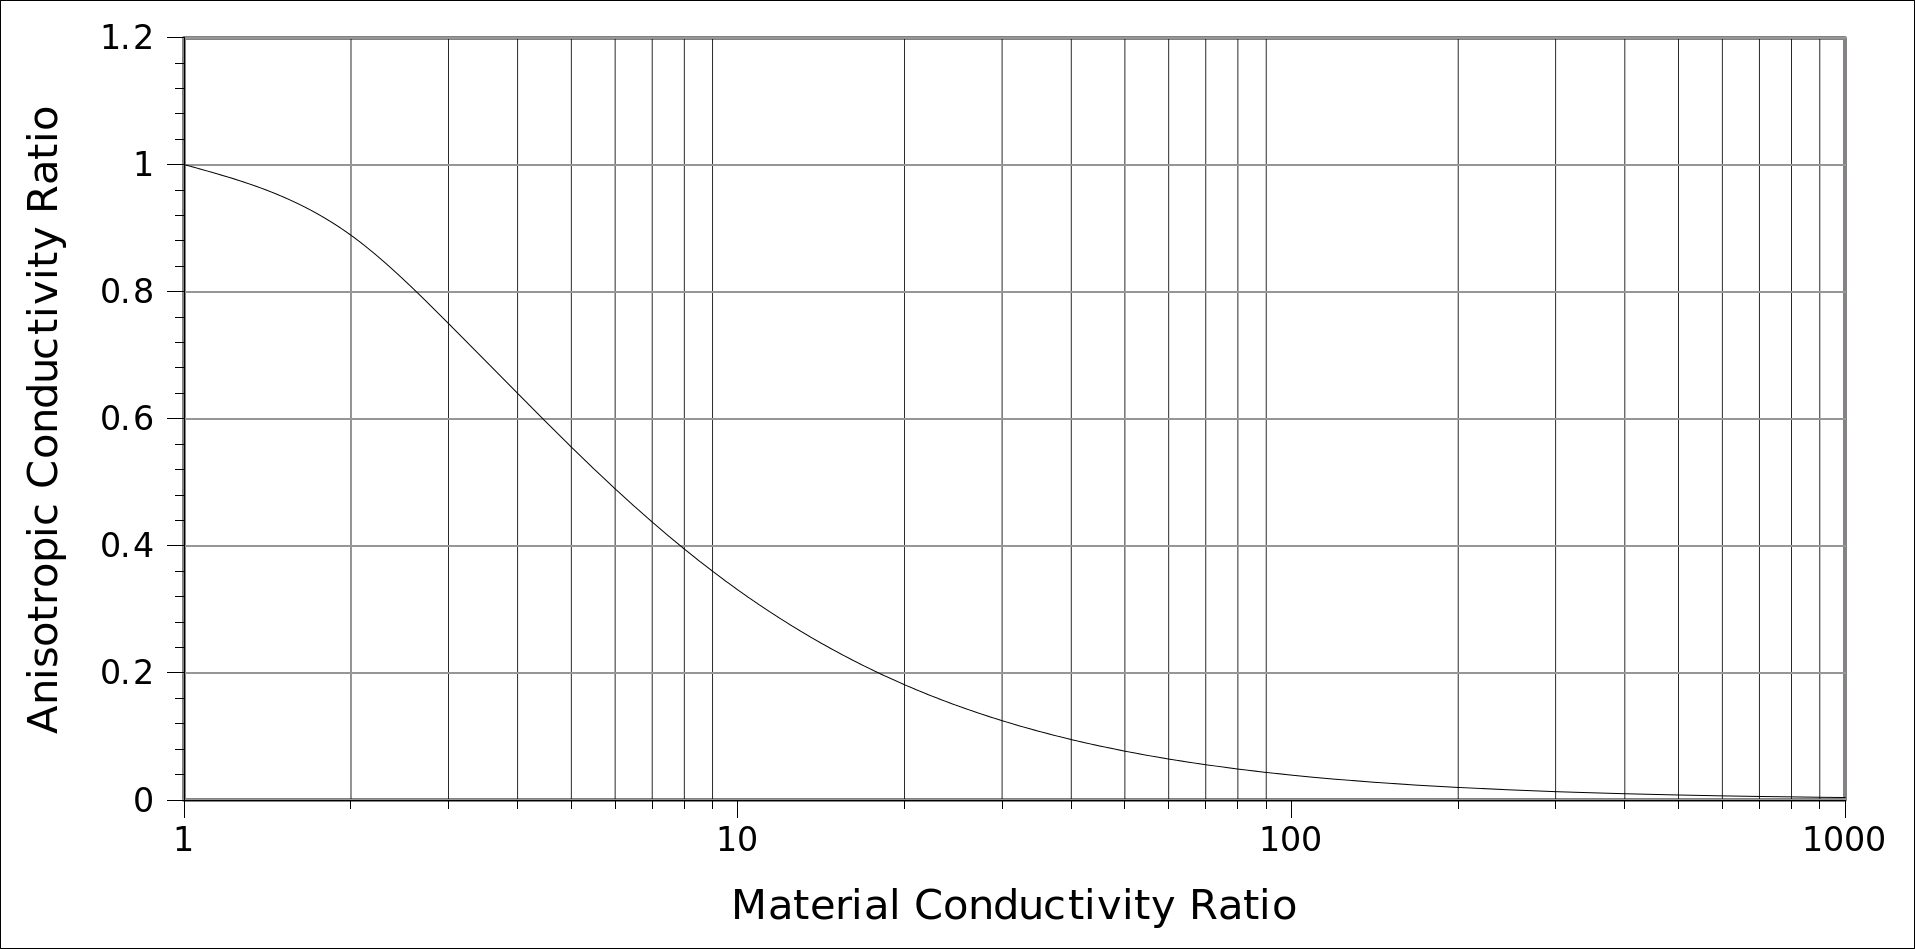
\includegraphics[width=0.7\textwidth]{fig/anisovmaterial_ratios.png}
\caption{Anisotropic Conductivity Ratio vs. Material Conductivity Ratio for the
layered geometry used in the benchtop experiments. It may take a very large
material conductivity ratio in order to achieve a relatively minor anisotropic
conductivity ratio.}
\label{fig:anisovmatl_rats}
\end{figure}

\section{Comprehensive Benchtop Measurements}

While enough benchtop measurements were taken to give a vague idea as to the
effectiveness of this measurement technique, there were not nearly enough
measurements to give a statistically valid conclusion regarding the slight
trend we were looking for. In addition to improving the benchtop method, there
need to be many more measurements taken, in order to draw statistically valid
conclusions.

\section{Comprehensive In-Situ Measurements}

The in-situ measurements presented in this document are very limited in scope.
One could easily spend much more time taking more measurements on more snow at
more angles, in order to better quantify the degrees of anisotropy in natural
snowpacks. More measurements would allow for a rigorous statistical analysis that
can show a trend with high confidence.


\section{Exploration of the Cooling Curve}

In the numerical and analytical models, the cooling curve is all but ignored. It
is believed that cooling curve models will yield analogous results, but this has
not been tested. Because of the importance of cooling curve measurements in the
real world (as they effectively double the number of measurements in a sample
and act as a consistency check on heating curve results),
verification of these expectations of analogous behavior should occur.

\section{A Method for Determining Anisotropic Thermal Conductivity From Measurements}

While this document lays the groundwork for determining anisotropic thermal
conductivity from measurements, a reliable method for converting measurements
into anisotropic thermal conductivities has not been found. This is, in part,
due to the discrepancy between the numerical and analytical approaches to
predicting effective thermal conductivity measurements as a function of angle
and degree of anisotropy, since the accuracy of the models is unknown.
Moreover, the lack of solid empirical data means that there is no evidence to
support either theory, outside of the isotropic case.

Given a reliable theory and data, one approach for ascertaining thermal
conductivity would be to find the degree of anisotropy for which the data as a
function of angle best fits the predicted \(k_{\textrm{eff}}\) curves
as a function of \(k_{xy}\) and \(k_z\).

One possibility is that, instead of focusing on the measured conductivities as a
function of angle, that one should focus on the \emph{change} in measured
conductivities with respect to angle. This is because, while the actual predicted
values for \(k_{\textrm{eff}}\) disagree, the predicted percent difference
between two measurements may be less so, particularly for instances of smaller
anisotropy ratios. In fact, given low enough degrees of
anisotropy, it may be sufficient to compare linearizations of
\(k_{\textrm{eff}}\) vs. \(\theta\) curves. Only with more research can this
conjecture be shown to be valid.

One suggestion for collecting data to determine the correct theory is to take
measurements at the most extreme angles possible. In the case of measuring
conductivity at the center of the snowpack, \(45\) degrees from horizontal is
about the practical limit. However, tests conducted at the top of the snowpack
would be able to record measurements at \(90\) degrees from horizontal, the angle
at which the other expected extreme value is expected to occur. Given this data,
determining the correct theory may be easier. The author recommends, in addition
to other measurements, that this experiment is conducted in future research.

\chapter{Conclusions}

An analytical model based on the isotropic solution outlined by
Carslaw and Yeager has been modified in order to predict thermal conductivity
measurements of anisotropic materials as a function of insertion angle.  This
model uses a linear transformation to pose the problem in a form equivalent to
the isotropic problem. However, in order to get meaningful results, the model
requires calculating the average temperature along an ellipse.

A 3-D finite element numerical model has also been built in order to predict
thermal conductivity measurements  of anisotropic materials as a function of
insertion angle. While the base model is simple by finite element model
standards, the number of parameters iterated through is somewhat unusual for
finite element modeling, and taxes the abilities of the software used.

According to both numerical and analytical theories, anisotropic thermal
conductivity should cause predictable changes in needle probe heating curve
measurements as a function of angle. While the two models show general
agreement, there are significant differences between the two predictions. These
may be explained by the 3D model's handling of edge effects, as well as possible
issues with the numerical model's convergence properties.

Measurements of engineered anisotropic materials are promising, but far from
complete. A basic, repeatable method has been designed and tested. The initial
results indicate the expected trend; however, due to the relatively low
amount of anisotropy in the material, the inherent noise in the thermal
conductivity measurement method and a disappointingly low amount of
measurements, a null hypothesis is impossible to rule out.

Similarly, in-situ measurements of snow have been made, but due to difficulties
in snow measurement very few useful data points were collected. However, the
results do suggest anisotropy in the snow.

Unfortunately, inquiry on this method is far from complete. Aside from the need
for more measurements, there are plenty of avenues for future researchers to
study.



\nocite{pratt}
\nocite{ewen}
\bibliographystyle{agufull08}
\bibliography{thesis}

\appendix
\chapter{Code Used in Chapter \ref{sec:analytical-np}}
\label{apx:analytical-np}

\section{model.py}

\small
\begin{minted}{python}
import json
from math import pi
from numpy import log, sin, cos, sqrt, array, \
                  arange, hstack, linspace, dot
from functools import reduce

def elliptical(fxn, ecc):
    from scipy.integrate import quad
    from math import pi
    from numpy import sin, cos, sqrt
    from types import FunctionType, BuiltinFunctionType

    #API trickery.
    if type(fxn) != FunctionType and type(fxn) != BuiltinFunctionType:
        fxn2 = lambda ecc, th: fxn
    else:
        fxn2 = fxn

    #The heavy lifting.
    return quad(lambda th: fxn2(ecc,th) *
                               sqrt( cos(th)**2.0 + (ecc*sin(th))**2.0 ),
                0, 2*pi)[0]

def Tavg(k_x, k_y, q, t):
    """
    given scalar r0, k_x, k_y and 1-d time, this returns a curve with
    the same slope at Tavg(t) for long T. May refactor.
    """
    return (4*pi*k_x/q)*array([elliptical(log(time) , k_x/k_y)/
                               elliptical(1, k_x/k_y) for time in t])

def kmeas(k_x, k_y, q, t):
    from numpy import polyfit
    """
    Does a quick linear curve fit 
    """
    return (q/4/pi)*polyfit(log(t), Tavg(k_x, k_y, q, t), 1)[0]


def rot(th, axis):
    from numpy.linalg import norm
    from numpy import sin, cos, eye, outer, cross
    if axis == "x":
        axis = array([1,0,0])
    elif axis == "y":
        axis = array([0,1,0])
    elif axis == "z":
        axis = array([0,0,1])
    else:
        axis = axis/norm(axis)
    oh = outer(axis, axis)
    return oh + cos(th)*(eye(3) - oh) + sin(th)*cross(axis, eye(3))
    

def proj(matrix, rot):
    from numpy import eye, hstack, vstack, newaxis
    from numpy.linalg import eig
    return tuple(
               eig(
                   reduce( dot, [ vstack((
                                    hstack((
                                        eye(2),
                                        array([0, 0])[:, newaxis] )),
                                    array([0, 0, 0]))),
                                    rot,
                                    matrix,
                                    rot.T ]))[0])[0:2]


if __name__=="__main__":
    from numpy import diag, logspace, meshgrid
    from math import pi
    from progressbar import ProgressBar

    angles = range(0, 91) # Lots angles :D

    ks = arange(0.2, 0.4, 0.05) # Some ks
    (k_xy, k_z) = meshgrid(ks, ks)
    k_xy = k_xy.flatten()
    k_z = k_z.flatten()

    q = 0.5 #Like in sims
    t = hstack(( logspace(0.1,1.0,15),
                 logspace(1.0,3.0,15) ))

    results = []
    progress = ProgressBar()
    for th in progress(angles):
        for i in xrange(k_xy.shape[0]):
            (k_xp, k_yp) = proj( diag([k_xy[i], k_xy[i], k_z[i]]),
                                 rot(pi/180*(90-th), 'y'))
            results.append([ th,
                             k_z[i]/k_xy[i],
                             kmeas(k_xp, k_yp, q, t)/k_xy[i]])
    for row in results:
        print(', '.join(map(str, row)))
\end{minted}
\normalsize

\chapter{Code Used for Chapter \ref{sec:numerical-np}}
\label{apx:numerical-np}

\section{worker.m}
\small
\begin{minted}{matlab}
%worker.m
%does the working

function worker(kxy,kz)
    load('angles.mat', 'angles');
    angles
    [kxy,kz] = meshgrid(kxy,kz);

    % The commented-out ``flreport'' gives one the option of suppressing
    % graphical output from COMSOL. This is useful if one wants to run
    % COMSOL in a headless manner. Unfortunately, COMSOL 3.5a on the ARSC
    % systems has extreme difficulties running in headless batch mode.
    %flreport('off');

    params=struct('rsnow', 0.4, ...
                  'rneedle', 0.00025, ...
                  'lneedle', 0.1, ...
                  'density_snow', 200, ...
                  'density_needle', 8000, ...
                  'cp_snow', 2050, ...
                  'cp_needle', 460, ...
                  'q_needle', 0.5, ...
                  'k_needle', 160, ...
                  'time', [logspace(0.1,1,15) logspace(1,3,15)], ...
                  'angles', angles );

    saveroot=['./solutions-' date '/'];

    mesh = mesher(0,params);
    for angle=angles,
        try
            solutions = arrayfun(@(x,y) solver(x,y,mesh,angle,params), ...
                            kxy,kz, 'UniformOutput', false);
            save solutions
            fprintf('Fitting solutions...\n');
            solutions = {cellfun(@(tsd) {fitter(tsd{1}(1,:),tsd{1}(2,:), ...
                                             0.999,params), ...
                             tsd{1}, tsd{2}}, ...
                         solutions, 'UniformOutput', false)};
            fprintf('A solution set just completed.');
            system([ 'echo "A solution set finished on" `hostname` ' ...
                     '| mutt -s "A solution set completed." ' ...
                     'josh.holbrook@gmail.com' ]);
        catch exception
            system([ 'echo "Exception occurred on" `hostname` ' ...
                     '| mutt -s "Exception occurred--' exception.message ...
                     '" josh.holbrook@gmail.com' ]);
        end
        angles = angles(2:length(angles));
        save('angles.mat', 'angles');
        %solutions
        mkdir(saveroot);
        save([ saveroot 'solution-' num2str(angle) ], ...
             'solutions','angle','kxy','kz','params');
    end

    % Emails me when everything's done
    system([ 'echo "Results completed on " `hostname` ' ...
             '| mutt -s "Results Completed" ' ...
             'josh.holbrook@gmail.com' ]);
    system('touch down');
end
\end{minted}
\normalsize


\section{mesher.m}
\small
\begin{minted}{matlab}
% COMSOL Multiphysics Model M-file
% Generated in part by COMSOL 3.5a 
% (COMSOL 3.5.0.608, $Date: 2009/05/11 07:38:49 $)
% the rest of it modified by Joshua Holbrook

function fem=mesher(angle,params)
    % mesh_generate(angle)
    % generates a mesh for the given angle. 

    fprintf(['meshing for angle=' num2str(angle) '...\n']);
    flclear fem

    % COMSOL version
    clear vrsn
    vrsn.name = 'COMSOL 3.5';
    vrsn.ext = 'a';
    vrsn.major = 0;
    vrsn.build = 608;
    vrsn.rcs = '$Name: v35ap $';
    vrsn.date = '$Date: 2009/05/11 07:38:49 $';
    fem.version = vrsn;

    % Geometry
    g1=sphere3(num2str(params.rsnow), ...
               'pos',{'0','0','0'}, ...
               'axis',{'0','0','1'}, ...
               'rot','0');
    g2=cylinder3(num2str(params.rneedle), ...
                 num2str(params.lneedle), ...
                 'pos',{num2str(-params.lneedle/2),'0','0'}, ...
                 'axis',{'1','0','0'}, ...
                 'rot','0');
    parr={point3(0,0,0)};
    g3=geomcoerce('point',parr);
    parr={point3(params.rsnow,0,0)};
    g4=geomcoerce('point',parr);
    parr={point3(0,params.rsnow,0)};
    g5=geomcoerce('point',parr);
    parr={point3(0,0,params.rsnow)};
    g6=geomcoerce('point',parr);
    parr={point3(-params.rsnow,0,0)};
    g7=geomcoerce('point',parr);
    parr={point3(0,-params.rsnow,0)};
    g8=geomcoerce('point',parr);
    parr={point3(0,0,-params.rsnow)};
    g9=geomcoerce('point',parr);

    % Analyzed Geometry (?)
    clear p s
    p.objs={g3,g4,g5,g6,g7,g8,g9};
    p.name={'ORIGIN','PT1','PT2','PT3','PT4','PT5','PT6'};
    p.tags={'g3','g4','g5','g6','g7','g8','g9'};

    s.objs={g1,g2};
    s.name={'SNOW','NEEDLE'};
    s.tags={'g1','g2'};

    fem.draw=struct('p',p,'s',s);
    fem.geom=geomcsg(fem);


    % ODE Settings
    clear ode
    clear units;
    units.basesystem = 'SI';
    ode.units = units;
    fem.ode=ode;


    % Initialize mesh
    fem.mesh=meshinit(fem, ...
                      'hauto',5, ...
                      'hgradsub',[2,1.1], ...
                      'hmaxsub',[2,0.0005]);

    % Refine mesh
    fem.mesh=meshrefine(fem, ...
                        'mcase',0, ...
                        'rmethod','longest');

    fem=multiphysics(fem);
end
\end{minted}
\normalsize

\section{solver.m}
\small
\begin{minted}{matlab}
% COMSOL Multiphysics Model M-file
% Generated by COMSOL 3.5a 
% (COMSOL 3.5.0.608, $Date: 2009/05/11 07:38:49 $)

function answer=solver(kxy,kz,fem,theta,params)
    % solver(kxy,kz,mesh,params)
    % uses comsol to pump out a solution using a given mesh-mat
    % and a k-matrix in comsol format.

    fprintf(['solving for kxy=' num2str(kxy) ...
             ' and kz=' num2str(kz) '...\n']);
    % Application mode 1
    clear appl
    appl.mode.class = 'GeneralHeat';
    appl.module = 'HT';
    appl.shape = {'shlag(1,''J'')','shlag(2,''T'')'};
    appl.sshape = 2;
    appl.assignsuffix = '_htgh';
    clear bnd
    bnd.type = {'q0','cont'};
    bnd.shape = 1;
    bnd.ind = [1,1,1,1,2,2,2,2,2,1,1,1,1,2];
    appl.bnd = bnd;
    clear equ
    equ.sdtype = 'gls';
    % densities
    equ.rho = {params.density_snow,params.density_needle};
    equ.init = 0;
    equ.shape = 2;
    % Heat capacities
    equ.C = {params.cp_snow,params.cp_needle};
    % Wattage
    equ.Q = {0,params.q_needle/pi/(params.rneedle)^2};
    % Heat conductivities
    arr = [cos(theta*pi/180), 0, sin(theta*pi/180);
           0, 1, 0;
           -sin(theta*pi/180), 0, cos(theta*pi/180)]; %rotation matrix
    equ.k = {symmetric_tocell( ...
                 arr*diag([kxy,kxy,kz])*(arr')), ...
                 params.k_needle};
    equ.ind = [1,2];
    appl.equ = equ;
    fem.appl{1} = appl;
    fem.frame = {'ref'};
    fem.border = 1;
    fem.outform = 'general';
    clear units;
    units.basesystem = 'SI';
    fem.units = units;

    % Coupling variable elements
    clear elemcpl
    % Integration coupling variables
    clear elem
    elem.elem = 'elcplscalar';
    elem.g = {'1'};
    src = cell(1,1);
    clear bnd
    bnd.expr = {{'T',{}},{'1',{}}};
    bnd.ipoints = {{'4',{}},{'4',{}}};
    bnd.frame = {{'ref',{}},{'ref',{}}};
    bnd.ind = {{'1','2','3','4','10','11','12','13'}, ...
               {'5','6','7','8','9','14'}};
    src{1} = {{},{},bnd,{}};
    elem.src = src;
    geomdim = cell(1,1);
    geomdim{1} = {};
    elem.geomdim = geomdim;
    elem.var = {'int_T','area'};
    elem.global = {'1','2'};
    elemcpl{1} = elem;
    fem.elemcpl = elemcpl;

    % ODE Settings
    clear ode
    clear units;
    units.basesystem = 'SI';
    ode.units = units;
    fem.ode=ode;

    % Multiphysics
    fem=multiphysics(fem);

    % Generate GMG mesh cases
    fem=meshcaseadd(fem,'mgauto','anyshape');

    % Extend mesh
    fem.xmesh=meshextend(fem);

    % Solve problem
    fem.sol=femtime(fem, ...
                    'solcomp',{'T'}, ...
                    'outcomp',{'T'}, ...
                    'blocksize','auto', ...
                    'tlist', params.time, ...
                    'estrat',1, ...
                    'tout','tlist', ...
                    'linsolver','gmres', ...
                    'itrestart',100, ...
                    'prefuntype','right', ...
                    'prefun','gmg', ...
                    'prepar',{'presmooth','ssor','presmoothpar',{'iter',3,'relax',0.8},'postsmooth','ssor','postsmoothpar',{'iter',3,'relax',0.8},'csolver','pardiso'}, ...
                    'stopcond','0.06-int_T/area', ...
                    'mcase',[0 1]);

    % Save current fem structure for restart purposes
    fem0=fem;

    % Plot solution
    %{
    postplot(fem, ...
             'slicedata',{'T','cont','internal','unit','K'}, ...
             'slicexspacing',5, ...
             'sliceyspacing',0, ...
             'slicezspacing',0, ...
             'slicemap','Rainbow', ...
             'solnum','end', ...
             'title','Time=100    Slice: Temperature [K]', ...
             'grid','on', ...
             'campos',[-2.636014311828346, ...
                       -3.4353207343472505, ...
                       2.4999999999999996], ...
             'camtarget',[0,0,0], ...
             'camup',[0,0,1], ...
             'camva',41.213465344831754);
    %}

    % Integrate
    T_thermistor=postint(fem,'T', ...
               'unit','K', ...
               'recover','off', ...
               'dl',8, ...
               'edim',0, ...
               'solnum','all');

    % Integrate
    T_surf_avg=postint(fem,'T', ...
               'unit','', ...
               'recover','off', ...
               'dl',[1,2,3,4,10,11,12,13], ...
               'edim',2, ...
               'solnum','end');

    answer={[fem.sol.tlist; T_thermistor],T_surf_avg};
    angles = params.angles(2:length(params.angles));

    %flsave(['fem-' num2str(theta) '-' num2str(kxy) ...
    %        '-' num2str(kz) '.mph']);

    save('angles.m', 'angles');
end
\end{minted}
\normalsize

\section{fitter.m}
\small
\begin{minted}{matlab}
function k = fitter(t,T,rset,params)
    logt = log(t(t>1));
    T = T(t>1);

    disp('Finding linear portion...');    
    for i=1:length(logt)-1
        C = corrcoef(logt(i:length(logt)), T(i:length(T)));
        r = sqrt(C(2,1));
        if r > rset %adjust this to get 'good' values
            disp(['linear fitting to ' num2str((length(logt)-i)) ...
                  ' points from t=' num2str(exp(logt(i))) ...
                  ' to t=' num2str(exp(logt(length(logt)))) '...']);
            x = polyfit(logt(i:length(logt)),T(i:length(T)), 1);
            break
        end
    end

    %plot(logt,T,'*');
    %hold on;
    %plot(logt, x(1)*logt + x(2));
    k = (params.q_needle)/(4*pi*x(1));

end
\end{minted}
\normalsize

\section{assembler.m}
\small
\begin{minted}{matlab}
function answers=assembler(directory)
    cd(directory);
    d = dir();
    answers = [];
    for i=3:length(d),
        disp(['Opening ' d(i).name '...']);
        load(d(i).name);
        answers = [answers, solutions];
    end
    cd('..');
end
\end{minted}
\normalsize

\section{reFitter.m}
\small
\begin{minted}{matlab}
function fixed=reFitter(broked, r, params)
    fixed = broked;
    for i=1:length(fixed),
        fixed{i} = cellfun(@(kset) { ...
            fitHelper(kset{2}, r, params), ...
            kset{2}, kset{3}}, fixed{i}, 'UniformOutput', false);
    end
end

function fitted=fitHelper(tT, r, params)
    fitted = fitter(tT(1,:),tT(2,:),r, params);
end
\end{minted}
\normalsize

\section{analyzer.m}
\small
\begin{minted}{matlab}
%analyzer
%Does some analyzing of the simulation results
%breaks for [kxy,kz] != meshgrid(ks,ks)

%Solutions location
%load solutions-19-Sep-2010/solutions-all.mat;

%Things I already know :)
%ks = linspace(0.2, 0.4, 6);
%ks = [0.2,0.4];
%[kxy, kz] = meshgrid(ks, ks);
%[kzy, kz] = meshgrid(0.3, 0.5);
%ks = 1;
%angles = 0:15:90;
%angles = 0:5:90;
%angles = [0 90];

%For an obvious color gradient, from red to blue right now.
colores = @(i,n) [sin((i/n)*pi/2), 0, cos((i/n)*pi/2)];

disp(['Showing overlaid plots (YES ALL OF THEM)' ...
      ' to make sure they "look" right:']);
figure;
hold on;
for theta = 1:length(angles)
    for i=1:length(ks)^2


        tT = answers{theta}{i}{2};
        plot(log(tT(1,tT(1,:) > 1 )),tT(2,tT(1,:) > 1), ...
             'color', colores(i,length(ks)^2));
    end
end

disp('Sanity checking results for isotropic cases');
figure;
hold on;
kmsold = 0 * cellfun(@(prison) prison{1}, answers{1});
for i=1:length(angles)
    %Extracts all the measured k's from the data
    % "prison" refers to cell representing particular
    % k combination in answers{theta}
    kms = cellfun(@(prison) prison{1}, answers{i});
    if kms == kmsold,
        disp('wtf exactly equivalent kms''s');
    end
    %diag(kms)
    %diag(kxy)
    errs = 100*(diag(kms) - diag(kxy))./diag(kxy);
    %Not necessary to be 3d anymore :)
    plot3(diag(kxy), errs, angles(i)*ones(size(diag(kxy))), ...
          '*-', 'color', colores(i,length(angles)) );
    xlabel('k_{actual}');
    ylabel('error (%)');
    zlabel('angle (degrees)');
end

disp('Figuring out T_surf_avg at time T:');
%figure;
%hold on;
for theta=1:length(angles)
    tavgs = cellfun(@(prison) prison{3}, answers{theta});
    try
        assert(all(all(tavgs< 0.001)));
    catch
        disp(['Warning: average surface temps are a bit high' ...
              ' at theta=' num2str(angles(theta))] );
        disp(tavgs);
    end
    if theta == length(angles)
        figure;
        hold on;
        contourf(kxy,kz,tavgs);
        colorbar;
        colormap('pink');
        title(['Average Surface Temperature at End of '...
               'Heating Curve Simulation for a representative angle');
        xlabel('K_{xy}');
        ylabel('K_{zz}');
    end
end

%dimensions changed to be in order kxy, then
%rows are angle and columns are kzz
disp('Plotting k_{meas}/k_{xy} vs. \theta and k_{z}/k_{xy}...');
kms=cell(size(ks));
for i=1:length(angles)
    kmsbyangle = cellfun(@(prison) prison{1}, answers{i});
    for j=1:length(ks)
        %Normalize by particular kxy
        kms{j} = [kms{j}; kmsbyangle(:,j)'/ks(j)];
    end
end
figure;
hold on;
[kgrid, anggrid] = meshgrid(ks, angles);
for n=1:length(ks)
    x = reshape(anggrid',[],1), reshape(kgrid'/ks(n),[],1)
    y = reshape(kms{n}',[],1)
    plot3(x, y, '*-', 'color', colores(n, length(ks)));
end
%legend(arrayfun(@(x) num2str(x),ks, 'UniformOutput', false));
xlabel('angle (degrees)');
ylabel('k_{zz}/k_{xy}');
zlabel('k_{meas}/k_{xy}');
\end{minted}
\normalsize

\section{tabulator.m}
\small
\begin{minted}{matlab}
%tabulator
%turns lame structures into some csv action

%given params:
%  answers
%  angles
%  kxy
%  kz

% Bad style, but I'm dealing with a cluttered namespace
% because I'm not functionalizing these.
% This is because parameter passing is annoying. So, leave me alone.
[Kxy, Kz] = meshgrid(kxy, kz);

fprintf('angle, kxy, kz, kmeas \n');
for t=1:length(angles),
    for pt=1:size(Kxy,1)*size(Kxy,2),
        fprintf([ num2str(angles(t)) ', ' ...
                  num2str(Kxy(pt)) ', ' ...
                  num2str(Kz(pt)) ', ' ...
                  num2str(answers{t}{pt}{1}) '\n']);
    end
end
\end{minted}
\normalsize

\section{symmetric\_tocell.m}
\small
\begin{minted}{matlab}
function a=symmetric_tocell(A)
    % Converts a symmetric matrix A into a cell 
    % containing the values, comsol-style.
    % I need to make sure comsol likes them nx1 instead of 1xn.

    %test for squareness
    assert(size(A,1)==size(A,2), ...
           'Dawg that matrix aint square much less symmetric');
    %test for symmetry
    for i=1:size(A,1),
        for j=i:size(A,1),
            if (A(i,j)~=A(j,i)),
                disp(['Warning: Dawg that matrix aint square (A(' ...
                      int2str(i) int2str(j) ')=' num2str(A(i,j)) ...
                      ' != A(' int2str(j) int2str(i) ...
                      ')=' num2str(A(j,i)) ' ! )']);
            end
        end
    end

    %The actual heavy lifting.
    a={};
    for m=1:size(A,1),
        %Takes upper-triangular section of mth column
        for element=A(1:m,m)'
            a{size(a,1)+1,1}=element;
        end
    end

end

function t=triangle(n)
    t=(n^2+n)/2;
end
\end{minted}
\normalsize


\chapter{Code Used for Chapter \ref{sec:irl}}
\label{apx:irl}

\section{testtools.py}

``testtools.py'' is a loose port of code written by Dr. Matthew Sturm for
IGOR Pro to do a similar analysis.

\small
\begin{minted}{python}
from __future__ import division

import tablib
from math import pi

# csv.reader and tablib aren't smart enough to read in numbers as numbers.
# Therefore, I map this over the strings in the rows spat out by csv.reader.
def str2num(string):
    import re

    if re.match('^-?\d*\.\d*$', string):
        return float(string)
    elif re.match('^-?\d+$', string):
        return int(string)
    else:
        return string


def import_raw_data(filename):
    import csv

    data = tablib.Dataset()
    for row in csv.reader(open(filename, 'r')):
        data.append( map(str2num, row) )

    data.headers = ( 'logger_id'
                   , 'day'
                   , 'hourmin'
                   , 'sec'
                   , 'needletemp'
                   , 'reftemp'
                   , 'volts'
                   , 'timer')

    return data

def unique(col):
    return list(set(col))


# Time is kept in two ints: one of the form hhmm, and the other in s.
# This function converts those to absolute seconds, and rebuilds the
# table appropriately.
def hms_to_s(data):
    # This bit here converts hhmm to seconds and adds to s.
    # It doesn't account for changes in the julian days.
    # Just don't test @ midnight, I guess.
    def convert(hourmin, sec):
        return 60*(hourmin%100) + sec + 3600*(hourmin//100 )

    def sieve(st):
        return (st != 'hourmin') and (st != 'sec')

    sec = map(lambda t: convert(t[0], t[1]), 
                   zip(data['hourmin'], data['sec']))

    new_data = zip(sec, *map( lambda h: data[h],
                               filter(sieve, data.headers) ))
    new_headers = ['sec']+filter(sieve, data.headers)
    return tablib.Dataset(*new_data, headers=new_headers)


def tab_filter(data, header, testfxn):
    new_data = [];
    for (i, pt) in enumerate(data[header]):
        if testfxn(pt):
            new_data.append(data[i])
    return tablib.Dataset(*new_data, headers=data.headers)


def tab_pprint(data):
    width = 2 + max(map(lambda st: len(st), data.headers))

    def padder(st):
        l = len(str(st))
        return st + (width-l)*" " if l <= width else st[:width]

    print " | ".join(map(padder,data.headers))
    print "-"*((width+2)*len(data.headers)-1)
    for row in data:
        print " | ".join(map(padder,map(str,row)))


def tab_plot(data, x_header, y_headers = None, fit=None ):
    import matplotlib.pyplot as pyplot

    headers = filter(lambda h: h != x_header, data.headers if y_headers == None else y_headers)

    xs = [ data[x_header] for header in headers ]
    ys = [ data[header] for header in headers]


    if (fit != None):
        from numpy import arange, exp, log, polyval
        more_xs = arange(data[x_header][1],data[x_header][-1])
        more_ys = polyval(fit,log(more_xs))
        xs+=[more_xs]
        ys+=[more_ys]

    pyplot.semilogx(*reduce(lambda a, b: a+b, zip(xs,ys)))
    pyplot.xlabel(x_header)
    pyplot.ylabel('Everything Else')
    pyplot.show()
    return data


#Repeats code from hms_to_s, or whatever I called that fxn.
#Ideally, I would generalize the ideas of, "do something with
#these columns, generate THIS column" and "Get rid of these
#columns.
def relative_time(data, h_abs="sec", h_rel="sec"):
    from numpy import array

    t_actual = data[h_abs]
    t_zero = t_actual[0]

    t_relative = list(array(t_actual) - t_zero)

    def sieve(st):
        return (st != h_abs)

    new_data = zip(t_relative, *map( lambda h: data[h],
                                     filter(sieve, data.headers) ))

    new_headers = [h_rel]+filter(sieve, data.headers)

    return tablib.Dataset(*new_data, headers=new_headers)



#A class of tools for splitting data up
class Splitters(object):

    #You change your mind like a girl changes clothes!
    @staticmethod
    def hot_and_cold(data):
        from numpy import array, floor
        from scipy.optimize import curve_fit
       

        def fit(x, a, b, c):
            y = map(lambda x: (b if (x-a) > 0 else 0) - c, x)
            return array(y)

        split = int(floor(curve_fit(fit,
                                    data['sec'],
                                    data['volts'],
                                    ( 0.5*(data['sec'][0]+data['sec'][1]),
                                      data['volts'][0],
                                      0 ))[0][0]))

        hot = tablib.Dataset( *data[slice(None, split, None)], 
                              headers=data.headers)
        cold = tablib.Dataset( *data[slice(split, None, None)],
                              headers=data.headers)
        return ( hot, cold )

    @staticmethod
    def manual(data, header, value):
        a = tab_filter(data, header, lambda x: x < value)
        b = tab_filter(data, header, lambda x: x >= value)
        return (a, b)


def linreg(data, xheader = 'sec', yheader = 'needletemp' ):
    from numpy import polyfit, log
    return polyfit(log(data[xheader][1:]), data[yheader][1:], 1)


def q(data):
    from numpy import average

    # I'm not sure what these constants mean, but based on the equation
    # I can make a pretty good guess!
    r_r = 10.6 #needle radius?
    r_h = 142.2 #resistance?
    l = 0.120 #needle length?

    volts = float(average(data['volts']))

    return ((volts/1000)**2.0 * r_h) / (l*r_r**2.0)


def heating_curve(data, q):
    const = linreg(data)[0]
    return q/4.0/pi/float(const)


def cooling_curve(cool_data, q):
    const = linreg(cool_data)[0]
    return -q/4/pi/float(const)


#applies mcgaw cooling curve. Untested.
def mcgaw(data, k_hot, q_hot, hot_period):
    from math import exp, log, pi

    correction = 4*pi*q_hot*k_hot*log( (exp(data['sec'][-1])+ hot_period) /
                                       hot_period)

    #print data['sec'][-1]
    #print hot_period
    #print correction

    newtemps = map( lambda x: x - correction, data['needletemp'])


    new_data = [];
    new_headers = data.headers

    for header in data.headers:
        if header == 'needletemp':
            #print "ding!"
            new_data.append(newtemps)
        else:
            new_data.append(data[header])

    #transposition!
    new_data = zip(*new_data)

    return tablib.Dataset(*new_data, headers=new_headers)
    

#Lachenbruch's Time Correction from a 1957 paper.
#Haven't been able to find said paper. Whatever.
def lachenbruch(data, dt):
    from numpy import exp, log

    data['needletemp'] = list(log(exp(data['needletemp']) - dt))

    return data
\end{minted}
\normalsize

\section{Raw Results of Numerical Model}

\begin{table}
\caption{\(\theta = [0:5:90]\), \([k_{xy}, k_z] = [0.3, 0.5]\)}
\begin{tabular}{r l l | l}
Angle (degrees) & \(k_{xy}\) & \(k_z\) & \(k_{\textrm{meas}}\)\\
0 & 0.3 & 0.5 & 0.42503\\
5 & 0.3 & 0.5 & 0.42439\\
10 & 0.3 & 0.5 & 0.42439\\
15 & 0.3 & 0.5 & 0.41927\\
20 & 0.3 & 0.5 & 0.41927\\
25 & 0.3 & 0.5 & 0.41927\\
30 & 0.3 & 0.5 & 0.40758\\
35 & 0.3 & 0.5 & 0.40047\\
40 & 0.3 & 0.5 & 0.39267\\
45 & 0.3 & 0.5 & 0.38462\\
50 & 0.3 & 0.5 & 0.37641\\
55 & 0.3 & 0.5 & 0.37196\\
60 & 0.3 & 0.5 & 0.36418\\
65 & 0.3 & 0.5 & 0.36418\\
70 & 0.3 & 0.5 & 0.35754\\
75 & 0.3 & 0.5 & 0.35574\\
80 & 0.3 & 0.5 & 0.35574\\
85 & 0.3 & 0.5 & 0.35574\\
90 & 0.3 & 0.5 & 0.3589\\
\end{tabular}
\end{table}


\begin{table}
\caption{\(\theta=0\), \([k_{xy}, k_z] = meshgrid(linspace(0.2, 0.4, 4), linspace(0.2, 0.4, 4))\)}
\begin{tabular}{r l l | l}
Angle (degrees) & \(k_{xy}\) & \(k_z\) & \(k_{\textrm{meas}}\)\\
0 & 0.2 & 0.2 & 0.21614\\
0 & 0.2 & 0.26667 & 0.2492\\
0 & 0.2 & 0.33333 & 0.28009\\
0 & 0.2 & 0.4 & 0.30801\\
0 & 0.26667 & 0.2 & 0.25315\\
0 & 0.26667 & 0.26667 & 0.29095\\
0 & 0.26667 & 0.33333 & 0.32668\\
0 & 0.26667 & 0.4 & 0.35519\\
0 & 0.33333 & 0.2 & 0.28594\\
0 & 0.33333 & 0.26667 & 0.32836\\
0 & 0.33333 & 0.33333 & 0.36839\\
0 & 0.33333 & 0.4 & 0.40493\\
0 & 0.4 & 0.2 & 0.31911\\
0 & 0.4 & 0.26667 & 0.36629\\
0 & 0.4 & 0.33333 & 0.40706\\
0 & 0.4 & 0.4 & 0.44717\\
\end{tabular}
\end{table}

\begin{table}
\caption{\(\theta=[30:15:90]\), \(k_{xy} = 0.3\), \(k_z = [0.1:0.1:0.5]\)}
\begin{tabular}{r l l | l}
Angle (degrees) & \(k_{xy}\) & \(k_z\) & \(k_{\textrm{meas}}\)\\
30 & 0.3 & 0.1 & 0.23\\
30 & 0.3 & 0.2 & 0.28322\\
30 & 0.3 & 0.3 & 0.3296\\
30 & 0.3 & 0.4 & 0.3704\\
30 & 0.3 & 0.5 & 0.40758\\
45 & 0.3 & 0.1 & 0.26424\\
45 & 0.3 & 0.2 & 0.29853\\
45 & 0.3 & 0.3 & 0.3296\\
45 & 0.3 & 0.4 & 0.35806\\
45 & 0.3 & 0.5 & 0.38462\\
60 & 0.3 & 0.1 & 0.29307\\
60 & 0.3 & 0.2 & 0.31317\\
60 & 0.3 & 0.3 & 0.3296\\
60 & 0.3 & 0.4 & 0.34888\\
60 & 0.3 & 0.5 & 0.36418\\
75 & 0.3 & 0.1 & 0.31449\\
75 & 0.3 & 0.2 & 0.32006\\
75 & 0.3 & 0.3 & 0.3296\\
75 & 0.3 & 0.4 & 0.33925\\
75 & 0.3 & 0.5 & 0.35574\\
90 & 0.3 & 0.1 & 0.32201\\
90 & 0.3 & 0.2 & 0.32375\\
90 & 0.3 & 0.3 & 0.3296\\
90 & 0.3 & 0.4 & 0.33566\\
90 & 0.3 & 0.5 & 0.3589\\
\end{tabular}
\end{table}

\begin{table}
\caption{\(\theta=[0:30:90]\), \(k_{xy} = 0.3\), \(k_z = [0.1, 0.5]\)}
\begin{tabular}{r l l | l}
Angle (degrees) & \(k_{xy}\) & \(k_z\) & \(k_{\textrm{meas}}\)\\
0 & 0.3 & 0.1 & 0.19287\\
0 & 0.3 & 0.5 & 0.42503\\
30 & 0.3 & 0.1 & 0.23\\
30 & 0.3 & 0.5 & 0.40758\\
60 & 0.3 & 0.1 & 0.29307\\
60 & 0.3 & 0.5 & 0.36418\\
90 & 0.3 & 0.1 & 0.32201\\
90 & 0.3 & 0.5 & 0.3589\\
\end{tabular}
\end{table}

\begin{table}
\caption{\(\theta=[5:5:15]\), \(k_{xy} = 0.3\), \(k_z = [0.1, 0.5]\)}
\begin{tabular}{r l l | l}
Angle (degrees) & \(k_{xy}\) & \(k_z\) & \(k_{\textrm{meas}}\)\\
5 & 0.3 & 0.1 & 0.19429\\
5 & 0.3 & 0.5 & 0.42439\\
10 & 0.3 & 0.1 & 0.19643\\
10 & 0.3 & 0.5 & 0.42247\\
15 & 0.3 & 0.1 & 0.20301\\
15 & 0.3 & 0.5 & 0.41927\\
\end{tabular}
\end{table}

\chapter{Needle Probe Apparatus Directions}

\section{Taking A Measurement}

The apparatus is controlled using a keypad that enables one to communicate
with the data logger using Campbell ``star-codes.'' Initiating a test is a
matter of clearing and setting some registers using these star-codes.

In general, the apparatus is used like so:

\begin{enumerate}
\item Turn on the device.
\item Insert the needle into medium being measured.
\item Use star-codes to clear the first three registers. ``* 6 A'' accesses the
registers, and ``D \(n\)'' toggles the \(n\)th register. For example, to clear
the second register, press ``* 6 A D 2'' .
\item Turn on the first register by pressing ``* 6 A D 1''. This makes the
apparatus measure temperature.
\item Turn on the second register by pressing ``* 6 A D 2''. This turns on the
heating element, effectively starting the test.
\item Wait 20 minutes for test to complete.
\end{enumerate}

\section{CSV Headers}

Data from the Campbell instrument comes in the form of a .csv file. For this particular experiment, the columns (from left
to right) represent:

\begin{enumerate}
\item An instrument ID (constant in this case).
\item Ordinal day, out of 366. For example, March 17th is day 76.
\item hh:mm portion of timestamp. For example, 6:30pm is represented as 1830.
\item Seconds portion of timestamp.
\item Needle temperature, in Celcius.
\item Reference temperature, in Celcius.
\item Voltage across needle probe, in millivolts.
\item Experiment timer, in seconds.
\end{enumerate}


\end{document}
